% !TeX spellcheck = en_US
\title{Decision Methods and Models}
\author{Massimo Perego}
\date{}

\documentclass[11pt]{report}
\usepackage{graphicx} 
\usepackage{amsmath}
\usepackage{amssymb}
\usepackage{amsfonts}
\usepackage[hidelinks]{hyperref}
\usepackage[autostyle, english = american]{csquotes}
\usepackage[parfill]{parskip}
\MakeOuterQuote{"}

\usepackage{amsthm}
\usepackage{booktabs}
\usepackage{centernot}
\usepackage{cancel}
\usepackage[italiano, noline]{algorithm2e}
\usepackage{tcolorbox}
\usepackage{setspace}
\usepackage{xparse}
\usepackage{xcolor}
\usepackage{array}
\usepackage{tikz}
\usepackage{pgfplots}
\pgfplotsset{compat=1.18}
\usetikzlibrary{intersections}

\newtheorem{theo}{Theorem}
\newtheorem{coro}{Corollary}
%\theoremstyle{definition}
\newtheorem{definition}{Definition}

\DeclareMathOperator{\dist}{dist}
\DeclareMathOperator{\R}{\mathbb{R}}
\DeclareMathOperator{\N}{\mathbb{N}}
\DeclareMathOperator{\Z}{\mathbb{Z}}
\DeclareMathOperator{\I}{\mathcal{I}}
\DeclareMathOperator{\U}{\mathcal{U}}
\DeclareMathOperator{\supp}{Supp}

\renewcommand{\P}{\mathcal{P}}

\newcommand{\wpref}[1]{\preceq_{#1}}
\newcommand{\indiff}[1]{\text{Ind}_{#1}}
\newcommand{\spref}[1]{\text{Str}_{#1}}
\newcommand{\inc}[1]{\text{Inc}_{#1}}
\renewcommand{\dist}{\text{dist}}

\NewDocumentEnvironment{myalgo}{m +b}{%
	\begin{center}
		\begin{minipage}{#1\linewidth}
			\begin{tcolorbox}[colback=white,sharp corners,boxrule=.3mm]
				\begin{algorithm}[H]
					\setstretch{1.3}
					\SetArgSty{relax}
					\SetAlgoNoEnd
					\SetKwSty{texttt}
					#2
				\end{algorithm}
			\end{tcolorbox}
		\end{minipage}
	\end{center}
}{}

\newcolumntype{L}[1]{>{\raggedright\arraybackslash}p{#1}}

\begin{document}
	\maketitle
	\tableofcontents
	\newpage	
	
	\part{Decision Problems}
	
	% !TeX spellcheck = en_US
\chapter{Introduction}
\label{ch:intro}

\section{Terminology}
\label{sec:terminology}

A \textbf{system} is the portion of the world affected by the decision, it should allow different configurations, it should not be given once and for all, otherwise no decision would be possible. 

A \textbf{solution} or \textbf{alternative} is the combination of all controllable aspects of the system, and \textbf{outcome} or \textbf{scenario} the combination of all its uncontrollable aspects. 

A system combines controllable and uncontrollable aspects into a \textbf{configuration}. Each configuration is associated to an \textbf{impact}, that describes all aspects relevant for the decision.

\textbf{Decision-maker} or \textbf{stakeholder} refers to everybody who contributes to the choice of the alternative. The former indicates who takes part to the choice, while the latter also includes who does not participate but has interests at stake and could react to a disagreeable choice, exerting an indirect influence on the choice. 

With \textbf{preference}, we denote the relative satisfaction between impacts. 

A decision problem requires to \textit{choose an alternative}: 
\begin{itemize}
	\item so as to \textit{move the system into a configuration} 
	
	\item such that \textit{the decision-makers prefers its associated impact} to those of other configurations
	
	\item keeping into account that \textit{the actual configuration depends on the alternative, but also on the scenario}
\end{itemize}

A \textbf{decision problem} implies two fundamental conditions: 
\begin{itemize}
	\item \textbf{Freedom}, i.e., availability of different choices (otherwise there is no decision)
	
	\item \textbf{Rationality}, i.e., the existence of preference criteria (otherwise the choice cannot be motivated)
\end{itemize}

This is a concept different from the definition of "decision problem" typically given in computer science (problem which admits only two possible solutions, \textit{yes} or \textit{no}). The decision problems considered here can be considered special cases of optimization/search problems, whose solution is an object with the maximum value (or minimum cost). 

%TODO Check
The focus is on practical decisions where a large amount of data must be taken into account, many choices are possible and the cost of a wrong choice is high.

We want to discuss \textit{what makes a decision complicated}, present the mathematical models to describe complicated situations and present the methods to deal with such situations, while recognizing limits and errors of this approach.

\section{Modeling approach to decision}
\label{sec:modelingapproach}

The modeling approach to decision requires a series of intermediate passages: 
\begin{itemize}
	\item Building a model of the problem
	
	\item Solving the model with algorithms, i.e., formal methods
	
	\item Interpreting the solution, with suitable methods
\end{itemize}

The strategy is to first \textbf{make a model}, then \textbf{compute}, and \textbf{finally decide}. From a problem to a model, solved by an algorithm, then actions are taken based on the solution.

The \textbf{decision process} occurs in an \textbf{iterative correction approach}:
\begin{enumerate}
	\item \textit{Problem formulation:} delineate the system, identifying impacts and preferences (Objectives) on one hand, decision-makers and scenarios (Context) on the other
	
	\item \textit{Alternative identification:} define the set of feasible alternatives
	
	\item \textit{Alternative evaluation and choice:} evaluate the impact associated to each configuration (alternative and scenario) and choose an alternative based on the preferences of the decision-makers
	
	\item \textit{Decision implementation:} apply or simulate the alternative selected
	
	\item \textit{Monitoring and check:} observe the consequences of the decision; if unsatisfactory, make correction and repeat the process, introducing new scenarios, objectives, alternatives and evaluation methods
\end{enumerate}

\begin{center}
	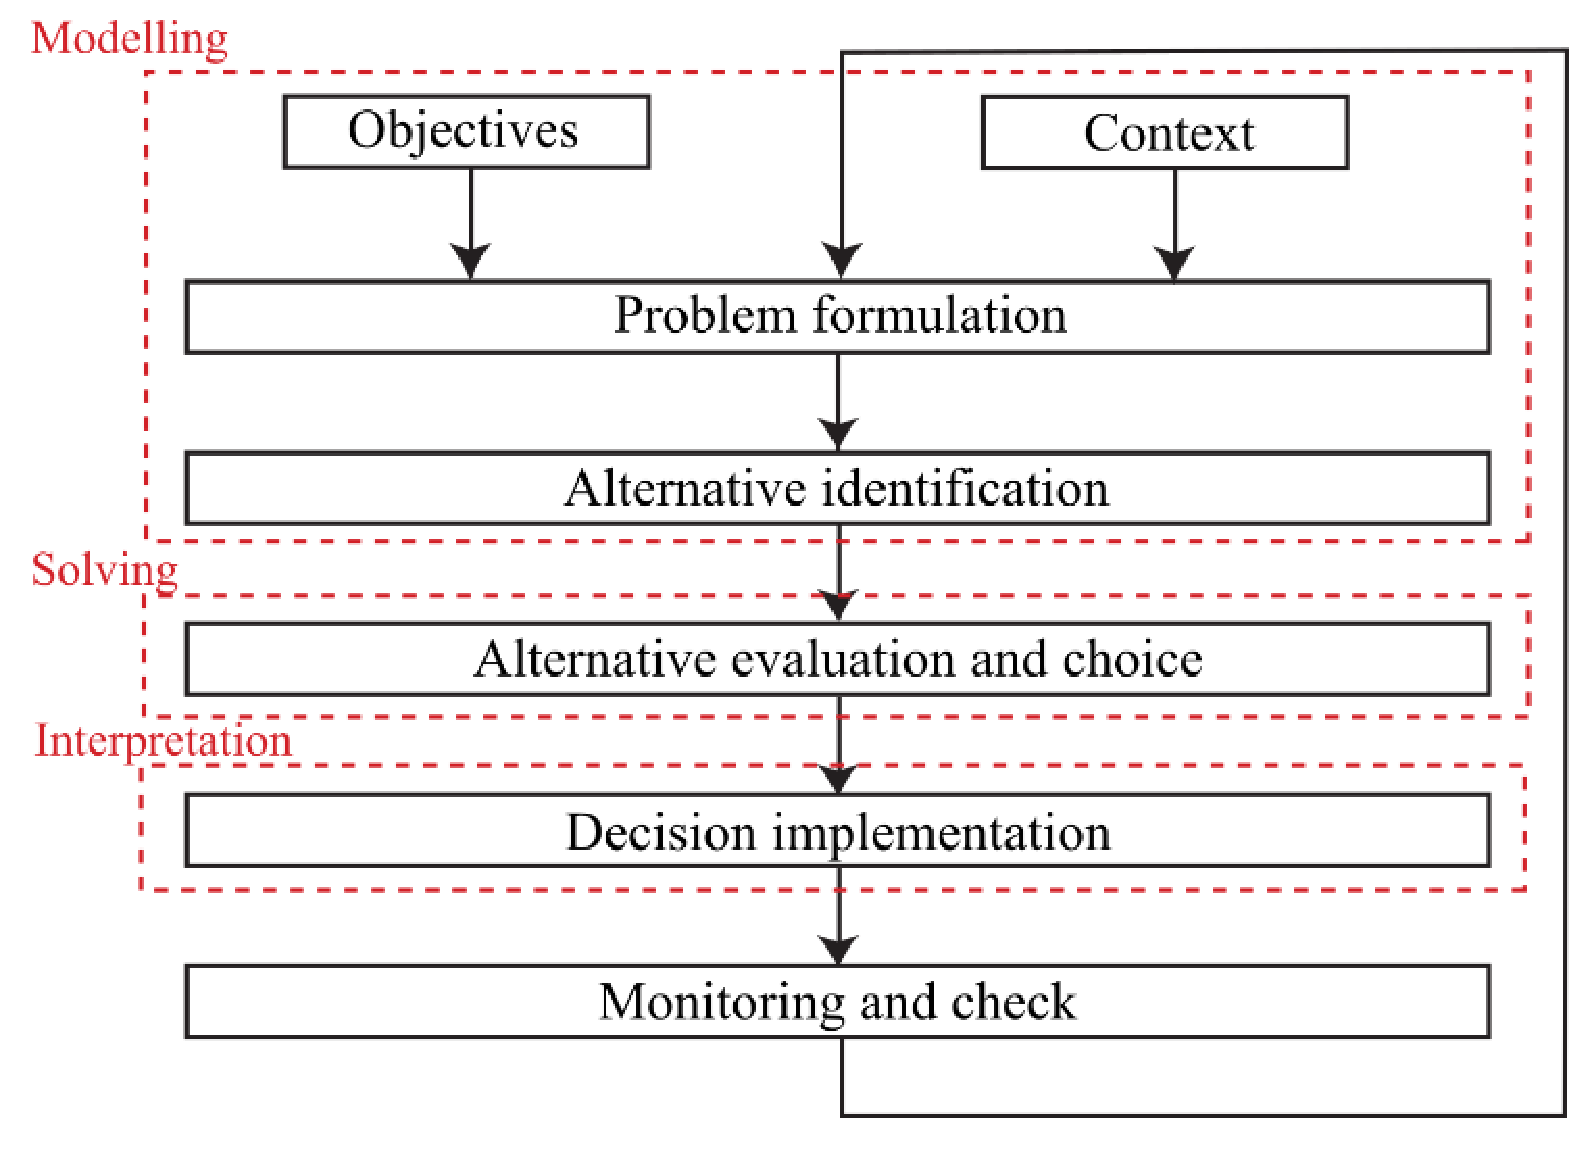
\includegraphics[width=0.75\columnwidth]{img/dp/intro/decisionIter}
\end{center}

\section{Why a formal approach?}
\label{sec:whyformal}

A formal approach allows to: 
\begin{itemize}
	\item Predict in a more certain and precise way the impact of a decision, using descriptive models instead of intuition and experience
	
	\item Accelerate the decision process, using algorithms and information technology
	
	\item Consider a much larger number of possible alternatives
	
	\item Clarifying and certifying the decision process
	\begin{itemize}
		\item making explicit the assumptions made on alternatives, scenarios, preferences and decision-makers
		
		\item guaranteeing repeatability of the process 
		
		\item allowing specific changes to the process, without starting from scratch
	\end{itemize}
\end{itemize}

The formal approach is based on
\begin{itemize}
	\item \textbf{Models}, to take decisions and predict their outcomes
	
	\item \textbf{Methods}, to build models, solve them, and interpret their results
\end{itemize}

\section{Prescriptive and descriptive models}
\label{sec:prescriptivedescriptive}

A decision model includes a number of sub-models, which can be classified based on the data they require and the result they produce. Decision models usually combine:
\begin{enumerate}
	\item \textbf{Prescriptive models} that
	\begin{itemize}
		\item receive impacts and preferences in input
		
		\item return a suggested alternative in output
	\end{itemize}
	\textit{if this is the case, you should do that}
	
	\item \textbf{Descriptive/predictive} models
	\begin{itemize}
		\item receive the system, an alternative and a scenario in input
		
		\item return an impact in output
	\end{itemize}
	\textit{If you do this and if this happens, you will obtain that}
\end{enumerate}

The two families of models can have subtle and complex interactions. For example, any prescriptive model uses a set of descriptive models to obtain the impacts of possible alternatives and scenarios; on the other hand, some descriptive models can include prescriptive ones.

Example: a model prescribes  a decision (\textit{close or open streets}) based on models that describe a system (\textit{amount of traffic}), including decisions prescribed by models (\textit{satellite navigators})

\section{What makes a decision problem complicated?}
\label{whycomplicated}

A decision problem can be \textit{complicated} due to:
\begin{itemize}
	\item An \textbf{insufficient model} of the system
	
	\item \textbf{Complicating features} of the model, such as
	\begin{itemize}
		\item complex preference structure, insufficient to define an optimum
		
		\item uncertain environment, impact depends also on unknown scenario
		
		\item multiple decision-makers, with potentially conflicting preferences
	\end{itemize}
	
	\item A \textbf{computationally complex model}, everything is clearly defined, but no efficient algorithm is known to solve the problem
\end{itemize}

The three main complexity sources for decision problems are: 
\begin{enumerate}
	\item \textbf{Preference structure}: simple or complex
	
	\item \textbf{Uncertainty}: a single scenario or many 
	
	\item \textbf{Decision-makers}: single or many
\end{enumerate}
giving rise to $2^3 = 8$ families of decision problems.

We'll consider four basic families of prescriptive models: 
\begin{enumerate}
	\item Simple preference, a single scenario and a single decision maker:
	\begin{itemize}
		\item mathematical programming
		
		\item multi-attribute utility theory
	\end{itemize}
	
	\item Complex preference, a single scenario and a single decision maker:
	\begin{itemize}
		\item paretian preferences
		
		\item weak rationality models (\textit{AHP} and \textit{ELECTRE} methods)
	\end{itemize}
	
	\item Simple preference, multiple scenarios and a single decision-maker:
	\begin{itemize}
		\item decisions in condition of ignorance (robust programming)
		
		\item decisions in conditions of risk (stochastic programming)
	\end{itemize}
	
	\item Simple preference, a single scenario and multiple decision-makers: 
	\begin{itemize}
		\item independent decision-makers (game theory)
		
		\item cooperating decision-makers (group decisions)
	\end{itemize}
\end{enumerate}

\subsection{Examples of complicated decision problems}
\label{subsec:examplesofcomplicatedproblems}

Before some large-size examples (Chapter \ref{ch:cases}), we present some realistic situations that might suggest what elements make a decision complicated in practice.

\paragraph{\textit{The search for parking:}} In a rather congested town, we are looking for a parking to leave out car and reach the place of an important meeting; we would prefer to park quickly  and not walk for long to reach the destination.
\begin{itemize}
	\item \textit{System} is the local street network, with the set of all potential parking places
	
	\item \textit{Alternative} is every possible trajectory of the car (path and time)
	
	\item \textit{Scenario} is every possible distribution of the free parking spaces over space and time
	
	\item \textit{Impact} are the driving time and walking time after parking
	
	\item \textit{Decision-maker} is the driver
\end{itemize}

The impact reduces to the aspects which actually matter for the decision, but it depends on a complex combination (configuration) of every possible trajectory of the car and distribution of parking spaces (alternative and scenario).

\paragraph{\textit{Thermostat regulation:}} We want to tune the classroom's thermostat so that the temperature is pleasant for the teacher and students.
\begin{itemize}
	\item \textit{System} is the classroom
	
	\item \textit{Alternative} is the position of the thermostat
	
	\item \textit{Scenario} is the external temperature and the exposition of the classroom to the sun 
	
	\item \textit{Impact} is the internal temperature of the classroom (but probably, also the humidity)
	
	\item \textit{Decision-makers} are all the people in the classroom (or just the teacher?)
\end{itemize}

This problem is easier than the others, but the definition of impact and decision-makers is not trivial.

\paragraph{\textit{Buying a car:}} We want to buy a car with good performance, comfort, design and low cost throughout its life cycle.
\begin{itemize}
	\item \textit{System} is the local market of cars, petrol, repairs, etc.
	
	\item \textit{Alternative} is the car bought 
	
	\item \textit{Scenario} are the stock and prices of the car dealers, the occurrence of accidents, prices of petrol and repairs, etc. 
	
	\item \textit{Impact} are the characteristics of the car throughout its life cycle
	
	\item \textit{Decision-maker} is the buyer (possibly some other family members/friends?)
\end{itemize}

A possible alternative, easy to forget, is to not buy a car, with an impact very bad for some aspects, but very good for others.

\paragraph{\textit{Risiko round:}} We want to play a round of Risiko, considering in turn all of the players.
\begin{itemize}
	\item \textit{System} is the map, with the distribution of territories, armies, cards
	
	\item \textit{Alternative} are the territories from which and to which each attack is launched and the corresponding number of attacking and defending armies
	
	\item \textit{Scenario} is the dices' outcome at each attack
	
	\item \textit{Impact} is the number of armies destroyed for each player
	
	\item \textit{Decision-makers} are the players
\end{itemize}

Here the presence of multiple decision-makers is intrinsic and unavoidable, moreover they all make their own choices autonomously.

	% !TeX spellcheck = en_US
\chapter{Case studies}
\label{ch:cases}

We want to present two case studies with the aim of clarifying the concept of complicated decision problems and to understand the practical meaning fo the terminology presented earlier. 

Both case studies concern large public works and could undergo several variations and corrections, as they are not yet implemented.

\section{The tramway of Como}
\label{sec:comotram}

\subsection{Context}
\label{subsec:comocontext}

Como has been for centuries at the center of exchanges, connecting Italy to Switzerland and Germany, while being a connection to cities at the end of the alpine valleys (Varese, Lecco, Bergamo, etc.).

This favorable position has led to problems, mainly related to saturation of the access ways, with congestion, economic losses due to slow transfers, pollution and accidents as a result.

Private cars are the main responsible for these problems, they concentrate on a few relatively small streets, which can't be enlarged easily due to the orography of the site.

A possible improvement could be to use public transport, more efficient from a transportation capacity point of view. However, the fraction of transfers serviced by public transport is small, and very uneven. Buses service a minority of users and are subject to the same limitations as private cars. 

As for train services, the state railway is rather unloaded (FS line), while the regional railway is nearly saturated (FNM line). How can the capacity of the FNM line be increased? Maybe while moving some of its passenger on the FS line.

Some critical points to consider while discussing interactions among the lines: 
\begin{enumerate}
	\item The crossing between the lines occurs with an acrobatic system of bridge: the Napoleona street overcomes the FNM line, which overcomes the FS line, which overcomes a small local street (Via dei Mulini)
	
	\item Between the stations of Camerlata and Borghi, the FNM line has a single track, with steep slopes on both sides
	
	\item Between the stations of Borghi and Lago, the FNM line has a single track, running along a narrow alley between houses
	
	\item Joining the FS and FNM lines through the town plain would require first to cross either the walls (in a historical area) or along the lakefront (touristy, occupied by a main street and flooded from time to time), and then climb the steep slope on top of which lies the FS station of Como S. Giovanni
\end{enumerate}
 
All these factors make a solution based on railways impossible to adopt, unless limited to the use of existing tracks. Increasing the frequency of the trains on the FNM line, however, has two problems: 
\begin{itemize}
	\item The single-track line forbids two trains to run along the Camerlata-Borghi-Lago track (unless perfect synchronization, difficult and prone to big problems)
	
	\item The levels crossing cut the town in two for several minutes every time a train passes along them, which could lead to significant traffic congestion
\end{itemize}

Hence the idea of a tramway line, which could: 
\begin{itemize}
	\item Have a double track, thanks to the shorter gauge
	
	\item Have fast crossing with traffic lights, instead of slow level crossings
	
	\item Be prolonged to the inside of town
\end{itemize}

But a classical tramway involves a big problem, as it requires to replace the whole track, therefore 
\begin{itemize}
	\item forcing train passengers from outside Como to change at an external station
	
	\item completely blocking traffic during the works
\end{itemize}

\subsection{The generation of the alternatives}
\label{sec:comoalternatives}

In this case, the set of alternatives is far from being clear. More correctly, it is \textit{indefinite}, and must be built step by step by investigating the whole context. 

We need to follow the iterative approach defined in Section \ref{sec:modelingapproach}. For instance, if one realizes that modifying the gauge of the tracks is too expensive, one can wonder if there exists tramways able to use standard train tracks. \href{https://it.wikipedia.org/wiki/Tram-treno}{\texttt{They exist}}.

The process of generating alternatives becomes easier if one decomposes the problem, identifying the basic \textit{alternative elements}, which can be (at least partly) independent.

In this study, three fundamental elements have been identified, in order to base on them the generation of alternatives: 
\begin{enumerate}
	\item The technology used to implement the new line 
	
	\item The route of the new line
	
	\item The management of the FNM trains with respect to the new line
\end{enumerate}

\paragraph{Technology} Previous studies on similar cases suggest three possible technologies:
\begin{enumerate}
	\item Standard railway service: add a shuttle-train between Grandate e Como Lago, so as to increase the frequency of the current railway service
	
	\item Tramway: replace the railway with a classic tramway
	
	\item Interoperable: add to the current railway service a special tramway which is able to work with both systems (facing all the resulting problems)
\end{enumerate}

\paragraph{Route} The number of possible routes is huge and not well-defined \textit{a priori}. To start, four possible routes have been identified: 
\begin{enumerate}
	\item Keeping the current FNM route, ending at the station of Como Lago 
	
	\item Linking the station of Como Lago (FNM) to Como S. Giovanni (FS) through new tracks crossing the town center
	
	\item Linking the station of Como Lago (FNM) to Como S. Giovanni (FS) through new tracks passing along the lakeside
	
	\item Building a ring around the town center through a new track from Como Lago (FNM) to Como S. Giovanni, plus a track from Como S. Giovanni (FS) to Como Borghi (FNM)
\end{enumerate}

\paragraph{Management of the FNM trains} This element of the alternatives describes the relation between the two rail transportation systems:
\begin{enumerate}
	\item Keep the FNM service on its current route
	
	\item Move the FNM service to the FS station of Como S. Giovanni, through the construction of an interchange between the FNM and FS lines (probably in the station of Camerlata)
\end{enumerate}

These are extreme possibilities, with a range of intermediate solutions, either during the works or permanently.

Each of these aspects provides an \textit{alternative element}. The single possible choices for an element can be associated to numerical values: sometimes a proper quantitative measure, other times simple arbitrary indices (e.g., 0 for the railway, 1 for the tramway and 2 for the interoperable). The purpose of this association, in general, is to describe effectively the set of alternatives, not to make computations.

Once the elements of the alternatives and the possible values for each element have been identified, one can proceed to enumerate their combinations, which in general are not all feasible. In the present case  there are $3 \cdot 4 \cdot 2 = 24$ combinations, only 7 of which are feasible. The other ones can be excluded due to obvious contradictions, technical impossibility or common sense. 

For example, the railway technology is incompatible with any route different from the present one (trains cannot go through towns).

A fundamental remark on the generation of alternatives is that \textbf{there always exists an alternative that consists in doing nothing} and keeping the current situation, this is conventionally denoted as \textbf{alternative zero}. New alternatives should, at least, not worsen the current situation. This is far from trivial since \textit{"worsen"} is a complicated concept.

In this discussion, we have neglected several other potential elements of alternative, such as
\begin{itemize}
	\item The location of interchange parking (in various sites)
	
	\item The implementation of double-tracks rails along parts of the current single-track rail
	
	\item The construction of new stations along the current route and possible new routes
	
	\item Possible transfers of the current route
	
	\item The extension of the service out of Como, beyond the station of Grandate
	
	\item The frequency of the new service
	
	\item The tariffs of the new service
	
	\item \dots
\end{itemize}

In particular, some mobility studies suggest that there could be a strong request for a railway servicing parts of the province currently badly connected to Como, both eastward and westward. Other subsequent feasibility studies have focused on these aspects, rejecting the most extreme solutions (current route and town ring), merging the intermediate ones (center crossing and lakeside route) in a mixed variant.

We also neglected the possible \textit{mitigation measures}, all those interventions that must be added to the alternatives in order to correct the negative impacts they produce, or to convince stakeholders strongly opposing the project to accept it (or at least not fight it too much), or to modify the impact of the work (e.g. limited access zones to discourage private cars).

All this confirms that even listing the possible solutions of a decision problem can be a preliminary problem in itself, that is not to be solved in a single phase, and actually is never ultimately solved.

\subsection{The generation of scenarios}
\label{subsec:comoscenarios}

The generation of scenarios follows the same rationale as the generation of the alternatives, also requiring to predict events uncontrollable by the decision-makers. First, one identifies the \textit{scenario elements} and their possible values, then we consider only the feasible combinations. If new scenarios emerge, or old ones disappear, the study should be updated and corrected.

The scenario elements considered are the following ones: 
\begin{enumerate}
	\item Closure of the lakeside to private traffic: forbidding the access of vehicles to the street that runs between the city center and the lake, this interacts with the project as it frees up the space used by cars, making it easier to build a tramway along the lakeside
	
	\item International Como-Chiasso station: it consists of merging the international railway stations of Como (Italy) and Chiasso (Switzerland) in a single stop, half-way, accelerating the trips between Italy and central Europe, this interacts with the project because the station of Como S. Giovanni would be reduced to the level of local station, introducing the need for a service taking travelers to Como S. Giovanni and possibly onward to the new international station
	
	\item Anti-flood barriers: it consists of building barriers that protect the center of Como from lake floodings, this interacts because a tramway service passing along the lakeside would be blocked by floods
	
	\item Borgovico tunnel: a toll tunnel that should run from the north-west to the south-west of Como, allowing to cross the town without congesting the western side
	
	\item Underlake tunnel: a tunnel which should run under the lake to replace the street that currently connects the north-west and nort-east of Como
\end{enumerate}

In theory, each combination of these elements is possible, excluding combining the underlake tunnel with keeping the lakeside open (meaningless) and building both tunnels (too expensive).

This discussion neglects important aspects such as: 
\begin{itemize}
	\item The anticipated variations in the residential and economic structure of the area under study
	
	\item The variations in the \textit{origin-destination matrix (O/D matrix)} of the potential transportation demand (i.e., the number of trips from place to place that will take place in the town and could be captured by the new service)
	
	\item The amount of European, state and region financing
\end{itemize}

Some of these scenario correspond to predictable numerical values, while others correspond to event which can either occur or not, or could occur in different ways. 

For each numerical value, for each event or for each way in which an event can occur, it could be possible to estimate a probability, or at least provide a qualitative estimation of its likelihood. All this information concurs to describe the set of possible scenarios and its auxiliary information.

\subsection{The definition and computation of the indicators}
\label{subsec:comoindicators}

As the alternatives and the scenarios, also the impacts are combinations of different elementary quantities, which are usually named \textit{indicators}. They characterize the satisfaction of the decision-makers for a configuration of the system, and determine their preferences. Indicators are typically much more numerous and diversified that the elements of the alternatives and the scenarios, so numerous that their generation adopts a hierarchical process that progressively details the sectors of the impact: 
\begin{itemize}
	\item Identify general macrosectors
	
	\item Each macrosector is decomposed into sectors, and possibly into sub-sectors, progressively more specific
	
	\item The elementary indicators are identified
\end{itemize}

This mechanism produces an \textit{indicator tree}. 

In this case, the three standard macrosectors used in Environmental Impact Assessment (EIA) have been adopted:
\begin{enumerate}
	\item \textit{Environment}, subdivided into Air pollution, Noise, Vibrations, Landscape and Territorial structure (that is, the compatibility with the current management plans of the area)
	
	\item \textit{Economy}, subdivided into Costs, Revenues and House values
	
	\item \textit{Society}, subdivided into Appreciation, Discomfort, Accessibility, Employment, Induced effects
\end{enumerate}

but a fourth macrosector has been added
\begin{enumerate}
	\setcounter{enumi}{3}
	\item \textit{Transportation}, subdivided into Security, Congestion and Interferences
\end{enumerate}

This last one is usually included in the Society macrosector, but it has been attributed an autonomous role as the study evaluates a large transportation service.

This yields the indicator tree:
\begin{center}
	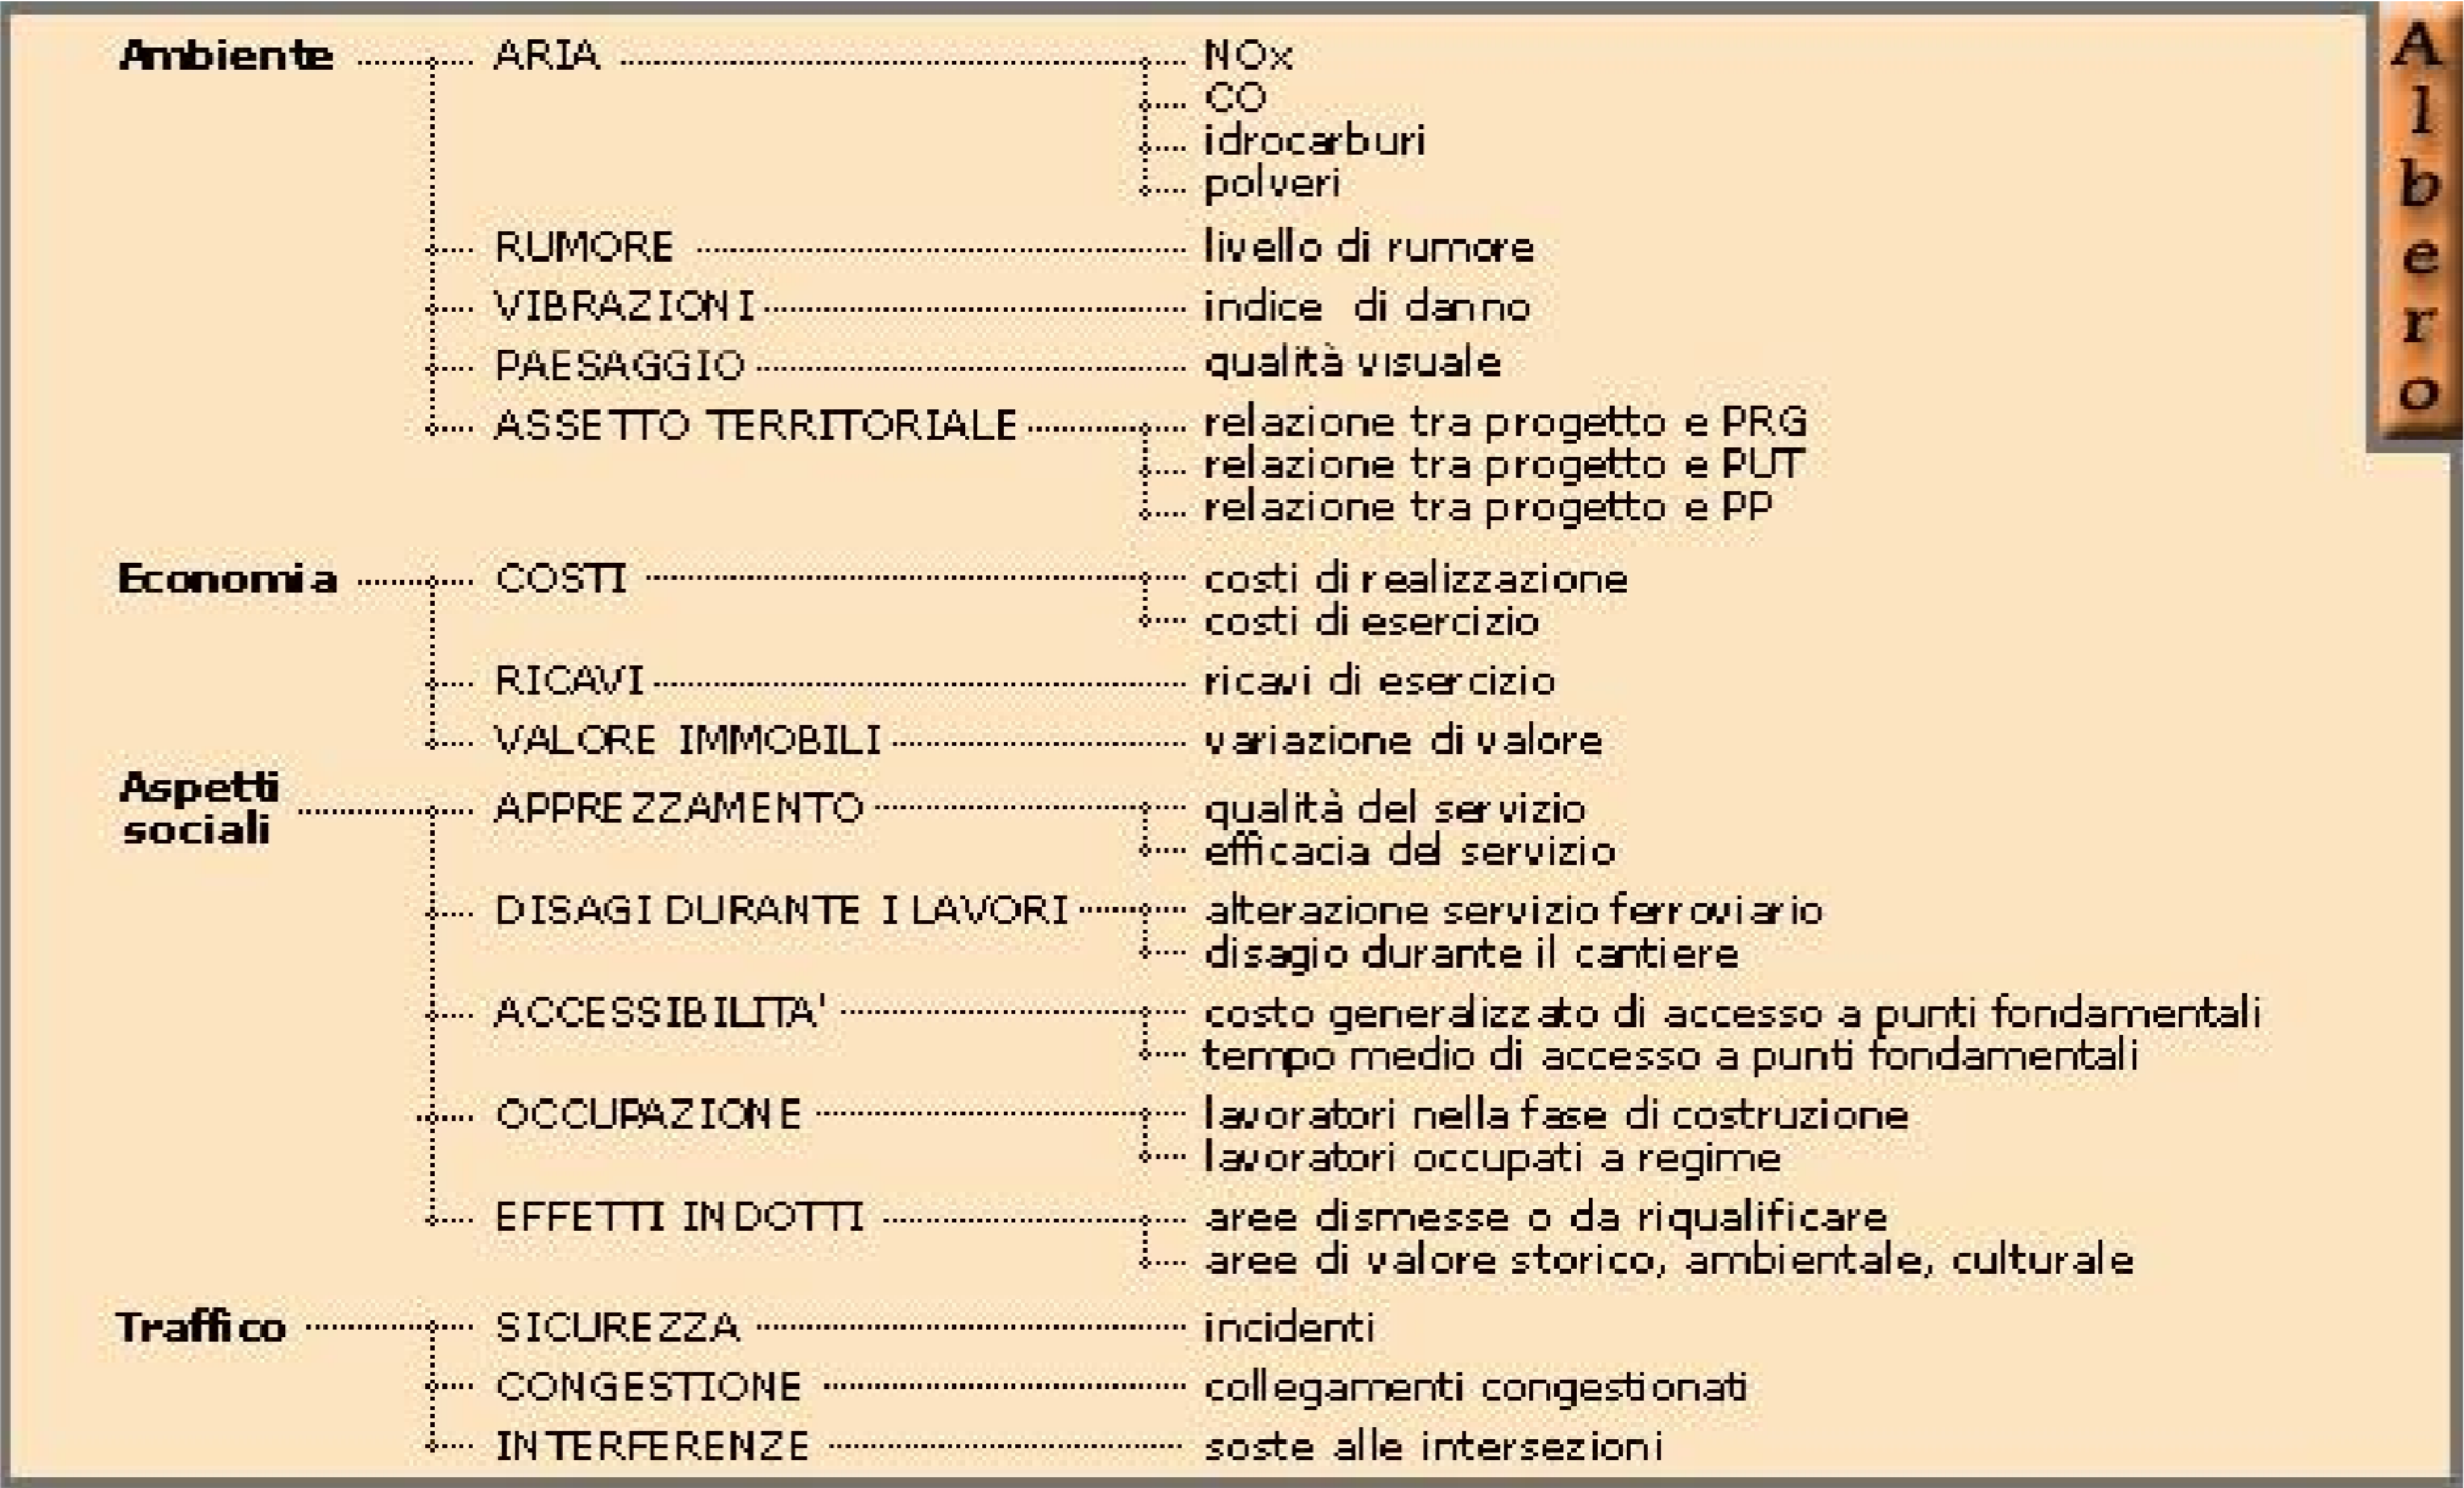
\includegraphics[width=0.98\columnwidth]{img/dp/cases/comotree}
\end{center}

The hierarchical structure aims to organize the evaluation of the single indicators during the phase of data collection; experts in each sector will be assigned to lead the estimation, prediction and measurement of the values of each indicator. 

Similarly, the construction of preferences in the decision phase will be organized based on the specific skills of experts of the various sectors; the "importance" of each indicator has to be determined.

Each indicator must be associated with a tool which will provide its values for each possible configuration. In most cases, these values will not be directly measurable, but are the result of estimates, given by a predictive model (e.g. $CO_2$ pollution can be measured now, but obviously not in all the hypothetical configurations).

The indicators can be numerical values that express physical measures, but also qualitative values on an ordinal scale. The purpose is not to make computations, just to describe the situation. In practice, some evaluation methods use such numerical values to make computations.

\paragraph{Time decomposition (phases) and space decomposition (zones)} Some indicators ave an intrinsic \textit{space} or \textit{time} feature, which must be taken into account; in other words, the values of an indicator might be meaningless if referred to the whole territory or whole time horizon of the project.

To correctly describe the situation, the system has to be divided into distinct geographical zones, on which is meaningful to define a value of the considered indicator.

This increases the amount of information to manage and requires to evaluate the relative importance of the different zones on the decision, as if they were values of different indicators. 

In this study, Como has been subdivided into 5 zones: 
\begin{itemize}
	\item Como centro 
	
	\item Borghi
	
	\item Camerlata
	
	\item Lora 
	
	\item Tavernola
\end{itemize}

Only the first three zones are directly affected by the project, whereas Lora and Tavernola have been maintained to check indirect effects on the whole town.

\subsection{The definition of the stakeholders}
\label{subsec:comostakeholders}

We denote as \textit{stakeholders} every person, organization, category or institution that is involved, directly or indirectly, in the project, even if it plays no role in the decision, since its interests are affected by the project.

The fundamental aspect in the description of stakeholders is to characterize their \textit{preferential structure}. However, the stakeholders could also point out neglected alternatives, scenario elements and indicators.

For this case, four classes of stakeholders have been identified: 
\begin{enumerate}
	\item Institutional stakeholders (Municipality, Province, Region)
	
	\item Society
	\begin{itemize}
		\item Citizens
		
		\item Environmentalists associations
		
		\item Category associations
	\end{itemize}
	
	\item Users
	\begin{itemize}
		\item Regular (commuters, students, etc.)
		
		\item Irregular
	\end{itemize}
	
	\item Transportation companies 
	\begin{itemize}
		\item FNM, whose track between Grandate and Como Lago should be used by the new service
		
		\item SPT, the local public transport company managing the bus lines, whose demand would be disrupted by the new service, requiring revision of routes and schedules
		
		\item FS, whose station of Como S. Giovanni could host part or all the trains currently servicing the FNM line
	\end{itemize}
\end{enumerate}

Each stakeholder has limited interests and skills, often related to one or few subtrees of the indicator tree, hence it will usually be involved mainly in the phases of the decision process which concerns those specific indicators. 

For this case, the relation between stakeholders and subsectors:
\begin{enumerate}
	\item The local government stakeholders will be interested in the whole system of indicators
	
	\item Concerning society stakeholders: 
	\begin{itemize}
		\item The citizen will probably focus their interest on the Environment, Society and transportation macrosectors
		
		\item The environmental associations will focus on the environmental macrosector
		
		\item The category associations (Camera di Commercio, Industria, Artigianato e Agricoltura, Confesercenti, \dots), who support the economic interests of the traders and entrepreneurs, will focus on the Economy macrosector and on the discomfort introduced by the works
	\end{itemize}
	
	\item The users will focus on the society macrosector, in particular on quality and accessibility of the service
	
	\item Concerning the transport companies
	\begin{itemize}
		\item FNM will focus on the Society (Emplyment and Discomfort) and Economy (Costs and Revenues) macrosectors
		
		\item SPT will focus on Society, Economy and Transportation macrosectors (Emplyment, Discomfrot, Traffico congestion and its own Costs and Revenues)
		
		\item FS is interested in the management of the train service potentially moved to the station of Como S. Giovanni
	\end{itemize}
\end{enumerate}

Once stakeholders have been identified, a reference person (or group) should be defined for each stakeholder, and involved in all phases of the decision process and subsequent iterations. 

The tools to interact with the person depend on the specific group of stakeholders considered; such tools could be talking with representatives of the group or polls, forms and interviews to the relevant subjects.

Some group of stakeholders can partly overlap (e.g. environmentalists and shopkeepers are also citizens), but the preference of common citizens will be different from those of a specific group, making it correct to represent them as different stakeholders.

\subsection{The decision process}
\label{subsec:comodecisionprocess}

For each possible configuration of the system it's necessary to evaluate each indicator, sometimes requiring physical measurements, but most of the time a suitable descriptive model can be applied to compute the expected value. Speaking in qualitative terms:
\begin{itemize}
	\item The alternatives exploiting the railway technology will have
	\begin{itemize}
		\item low implementation costs and low discomfort
		
		\item limited effect on the accessibility of sites not currently serviced
		
		\item limited environmental improvements
		
		\item nearly no impact on the employment
		
		\item \dots
	\end{itemize}
	
	\item The alternatives exploiting the "interoperable" technology will have
	\begin{itemize}
		\item higher economic costs
		
		\item stronger penetration of the service in the urban fabric, dependent on the chosen route
		
		\item intermediate discomfort
		
		\item \dots
	\end{itemize}
	
	\item The alternatives exploiting the classical tramway technology will have
	\begin{itemize}
		\item much higher implementation costs and times
		
		\item very detailed service
		
		\item \dots
	\end{itemize}
\end{itemize}

The resulting numerical and qualitative values will have to be aggregated depending on the preferences of the various stakeholders. It's necessary to model the preferential structure of each stakeholder, to determine preference among different impacts.

It is also necessary to aggregate the preferences of different stakeholders in a final ordering of the alternatives, or at least in the selection of one alternative. The \textit{sensitivity} of the final ordering should also be taken into account, that is the boundaries within which it remains valid when the data changes.

\section{Reopening of the Navigli in Milan}
\label{sec:navi}

\subsection{The context}
\label{subsec:navicontext}
Milan was born as a river town, rich in natural rivers, later further enriched by a network of canals. Modernity led to covering the whole network in favor of traffic and, more recently, to a periodic proposal and discussion of project to reopen part of it.

The main motivations for the project are:
\begin{itemize}
	\item The \textit{hydraulic continuity}, that is the possibility to better control and limit the flooding of water streams in the northern part of Milan, currently flowing through pipes, limiting the capacity and making cleansing more difficult
	
	\item The \textit{touristic and commercial navigability}, with their social, cultural and economic outcomes
	
	\item The \textit{production of electricity}, not by directly installing turbines in the Navigli, but with the increase of water flow in the Naviglio Pavese, which has several small hydroelectric plants south of Milan
	
	\item The \textit{feeding of heat-pump plants} in the area of Darsena using nappe (underground) water
	
	\item The \textit{decrease in the nappe level}, thanks to the extraction of water from wells which are currently closed, reducing the use of pumps in several underground stations that defend the tunnels from flooding
\end{itemize}

\subsection{The definition of the alternatives}
\label{subsec:navialternatives}

The definition of alternatives seems easier in this case, given the Navigli's well defined historical route. In practice, things are not easy.

Starting from a basic dichotomy, one can distinguish: 
\begin{itemize}
	\item "Virtual" alternatives, in which the Navigli are not actually reopened, but made enjoyable with public visual aids (sings, pavings, \dots)
	
	\item "Physical" alternatives, in which the Navigli are actually reopened
\end{itemize}

All physical alternatives do not share the same route, there are many alternatives: 
\begin{itemize}
	\item A partial reopening, keeping some covered stretches
	
	\item A complete reopening of the classic circle north-east-south, which includes a number of minor variations concerning
	\begin{itemize}
		\item Porta Nuova park
		
		\item Cavour Square
		
		\item the Vallone Naviglio
		
		\item the Viarenna basin
	\end{itemize}
	
	\item The reopening og the whole inner circle, also on the western side: some technical reasons make this alternative quite impractical (mainly, it interferes with underground line 2)
	
	\item Additional works with respect to the historical route:
	\begin{itemize}
		\item the Vettabbia canal
		
		\item the "Darsena 2" project, a brand new basin near the railway station Porta Genova
	\end{itemize}
\end{itemize}

Another fundamental element of the alternatives is navigability: the new canal could be open or closed to boat trips. The elements of alternative (route, navigability and other possible ones) must then be combines to build the alternatives, removing impossible combinations (virtual alternatives obviously forbid navigability).

\subsection{The definition of the scenarios}
\label{subsec:naviscenario}

This point is not developed in the project described, we therefore make a superficial analysis. The fundamental aspects of the scenario are:
\begin{itemize}
	\item Availability of public funding to build and manage the canal
	
	\item The (more or less) strict closure of the city center to private cars
	
	\item The construction of underground line 4 (completed as of writing) which would provide easy access on foot to most of the city center, even if private cars and some bus lines could not access it
\end{itemize}

\subsection{The definition and computation of the indicators}
\label{subsec:naviindicators}

We, once again, proceed in a hierarchical way, to identify large sectors and then dividing them. To give a non-exhaustive list:
\begin{itemize}
	\item Impact on pollution
	
	\item Variation of travel times to various parts of town
	
	\item Impact on traffic congestion
	
	\item Impact on public transport
	
	\item Construction costs
	
	\item The hedonic impact on the real estate prices
	
	\item Impact on commercial activities
\end{itemize}

Some of these impacts could be so negative as to introduce a feedback loop on the definition of the alternatives, a correction and update of the alternatives through the introduction of devices to reduce those impacts. E.g. bridges used by tramway can't have slopes, which implies a water level low enough and boat suitably designed in order to allow navigability.

\subsection{The time and space organization}
\label{subsec:navitimespace}

Several indicators are naturally related to geographical positions. Some indicators refer to zones, whereas others to linear stretches of the Naviglio. The detailed project divides the route of the canal into 16 stretches.

Concerning the time phases, some of them correspond, somehow, to alternatives, meaning it's  possible to implement a specific phase then leave the following "frozen" for a long time, waiting for favorable conditions to complete them. For example, virtual alternatives can be seen as a preliminary phase to a global reopening. They could achieve a partial result at low cost, however they could increase the overall cost.


The construction of a double Naviglio, with an underground pipe running under the canal is an additional cost, but it also allows to reach in short time the result of hydraulic continuity and to spread over time the following phases, dividing the expense.

\subsection{The definition of the stakeholders}
\label{subsec:navistakeholders}

The definition of the stakeholders is similar to what described in for the tramway of Como (\ref{subsec:comostakeholders}). The mayor of Milan can be considered as the decision-maker, but other subjects must be taken into account, such as transportation companies (mainly ATM, railway lines are not affected), the environmental and category associations, citizens. Among the citizens, the owners of real estate along the route of the canal could be considered specifically.

\subsection{The decision process}
\label{subsec:navidecision}

Once again, it's necessary to evaluate each indicator in each possible configuration. This implies the application of suitable descriptive models. One could expect that
\begin{itemize}
	\item The "virtual" alternatives will be particularly cheap and have negligible impact on traffic and pollution, but will not offer any advantage with respect to hydraulic continuity (unless combined with the construction of an underground pipe), to the production of electricity and to the management of water nappe, and they have limited impact on tourism and commerce; the aesthetic impact is harder to evaluate
	
	\item The "physical" alternatives will be much more expensive, reaching the objective of hydraulic continuity, electricity production, management of water nappe, while favoring tourism, commerce, real estate prices and aesthetic impact
\end{itemize}

Moreover
\begin{itemize}
	\item The alternatives involving a navigable canal will have touristic, commercial and accessibility advantages, but at a higher cost, requiring to manage a system of gatehouses to get over the height difference between subsequent stretches of the canal
	
	\item The alternatives involving a non-navigable canal will be cheaper, but less advantageous for accessibility, commerce and tourism, even if they could have a better aesthetic impact, since a navigable canal requires a relatively low water level to let boats pass under bridges
\end{itemize}

After all indicators have been evaluated, the aggregation phase can start, taking into account the preferential structure of all the stakeholders. This can be done in several ways and should conclude with an ordering of the alternatives, or at least the choice of one, also with the information on the sensitivity on such an ordering or choice.

% This should be L2

	% !TeX spellcheck = en_US
\chapter{Fundamental definitions and conceptual problems}
\label{ch:fundamentaldefinitions}

While analyzing the two case studies, we remarked that
\begin{itemize}
	\item The \textit{alternatives are generated combining elements of alternative} and there is always an alternative zero (leaving the system as is)
	
	\item The \textit{scenarios are generated combining elements of scenario}
	
	\item The \textit{impacts are generated combining indicators} and \textit{indicators are organized into a hierarchy}
	
	\item \textit{Each configuration generates an impact} through descriptive models
	
	\item \textit{Decision-makers should never ignore stakeholders} (people affected by the decision and can react to it)
	
	\item \textit{Preferences are expressed on impacts} (not on configurations)
\end{itemize}

\section{Decision problem}
\label{sec:decproblemdef}

\begin{definition}
	A \textbf{decision problem} is defined by a 6-uple
	$$ P = \left(X, \Omega, F, f, D, \Pi \right)$$
	where: 
	\begin{itemize}
		\item $X$ is the \textbf{feasible region}, the set of all alternatives; 
		
		\item $\Omega$ is the \textbf{sample space}, the set of all possible scenarios, or outcomes
		
		\item $F$ is the \textbf{indicator space}, the set of all possible impacts
		
		\item $f: X \times \Omega \rightarrow F$ is the \textbf{impact function}
		\begin{itemize}
			\item every pair $(x, \omega) \in X \times \Omega$ describes a configuration of the system on which a decision should be taken
			
			\item $f$ associates to each configuration $(x, \omega)$ of the system an impact $f(x, \omega) \in F$
			
			\item impact $f(x, \omega)$ describes all the features of the configuration $(x, \omega)$ that are relevant for the decision (costs, profit, quality levels, \dots)
		\end{itemize}
		
		\item $D$ is the \textbf{set of all decision-makers}, or stakeholders
		
		\item $\Pi: D \rightarrow 2^{F \times F}$ is the \textbf{preference function}, a function that associates to each decision maker $d \in D$ a subset of impact pairs $\Pi(d) \subseteq F \times F$; this is interpreted as a binary relation representing the preference of decision maker $d$
	\end{itemize}
\end{definition}

The aim of the problem is to identify a solution $x^\ast \in X$ or a subset of solutions $X^\ast \subseteq X$ that the decision-makers consider satisfactory based on their preferences between the impacts $f(x^\ast, \omega)$ with $\omega \in \Omega$ and the other impacts $f \in F$

\subsection{Alternatives}
\label{subsec:alternativesdef}

The alternatives formally describe the events under the control of the decision-makers. The set $X$ includes al the possible choices.

We'll assume that 
$$ X \subseteq \R^n \Leftrightarrow x = \left[x_1 \dots x_n \right]^T \text{ with } \ x_i \in \R \quad \forall i \in \{1, \dots, n\} $$
with a finite number $n$ of elements of alternative or decision variables. Real number can model several different situations (e.g. binary, enumerative, qualitative, quantitative, functions within families).

Several \textbf{kinds of feasible regions} $X$ exist
\begin{itemize}
	\item Continuous
	
	\item Discrete
	\begin{itemize}
		\item Infinite
		
		\item Finite
		\begin{itemize}
			\item Combinatorial (typically $|X| \in \Omega(d^n)$ for some $d > 1$)
			
			\item "Finite" (typically $|X| \in O(1)$)
		\end{itemize}
	\end{itemize}
\end{itemize}
Focusing on a specific kind allows algorithms which are more effective and less general.

The notation is, so far, purely descriptive and not used to make computations.

\subsection{Scenarios}
\label{subsec:scenariosdef}

The scenarios formally describe the events out of the control of the decision-makers that have non-indifferent effect on the system. The set $\Omega$ defines all such events during the time horizon relevant to the decision. Scenarios also describe modeling errors (disturbances).

We'll assume 
$$ \Omega \subseteq \R^r \Leftrightarrow \omega = \left[\omega_1 \dots \omega_r \right]^T \text{ with } w_k \in \R \quad \forall k \in \{1, \dots, r\} $$
with a finite number $r$ of elements of scenario or exogenous variables.

\subsection{Impacts}
\label{subsec:impactsdef}

The impacts formally describe all aspects that are relevant for the decision, i.e., decisions are taken based on the impact. 

The impacts are described quantitatively as vectors of real numbers. We'll assume 
$$ F \subseteq \R^p \Leftrightarrow f = \left[f_1 \dots f_p\right] \text{ with } f_I \in \R $$
with a finite number $p$ of 
\begin{itemize}
	\item indicators
	
	\item criteria
	
	\item attributes
	
	\item objectives
\end{itemize}

\subsection{Impact function}
\label{subsec:impactfunctiondef}

The impact function $f: X \times \Omega \rightarrow F$ is a vectorial function that associates each configuration $(x, \omega)$ to an impact $f(x, \omega)$. 

Trivial example
\begin{itemize}
	\item buy quantities $x_i$ of products ($n$ decision variables)
	
	\item Pay costs $\omega_i$ ($r = n$ exogenous variables)
	
	\item The total (mono-dimensional $p=1$) cost is $f(x, \omega) = \sum_{i=1}^n \omega_i x_i$
\end{itemize}

The impact function can be
\begin{itemize}
	\item a mathematical expression that describes a computation 
	
	\item a simulation or integration software
	
	\item an empirically generated graph or table
\end{itemize}

Two classical representations for finite problems are 
\begin{enumerate}
	\item The \textbf{evaluation matrix}
	\begin{center}
		\begin{tabular}{@{}l|rrrrrr@{}}
			\toprule
			\(f(x,\omega)\) & \(f_1\) & \(f_2\) & \(f_3\) & \(f_4\) & \(f_5\) & \(f_6\) \\
			\midrule
			\((x',\omega')\)   & 10 &  5 & 40 & 20 & 24 & 180 \\
			\((x',\omega'')\)  & 16 & 10 & 60 & 16 & 20 & 190 \\
			\((x'',\omega')\)  & 20 &  6 & 23 &  8 & 17 & 230 \\
			\((x'',\omega'')\) & 24 &  8 & 50 & 12 & 10 & 100 \\
			\bottomrule
		\end{tabular}
	\end{center}
	
	\item The \textbf{radar chart}
	\begin{center}
		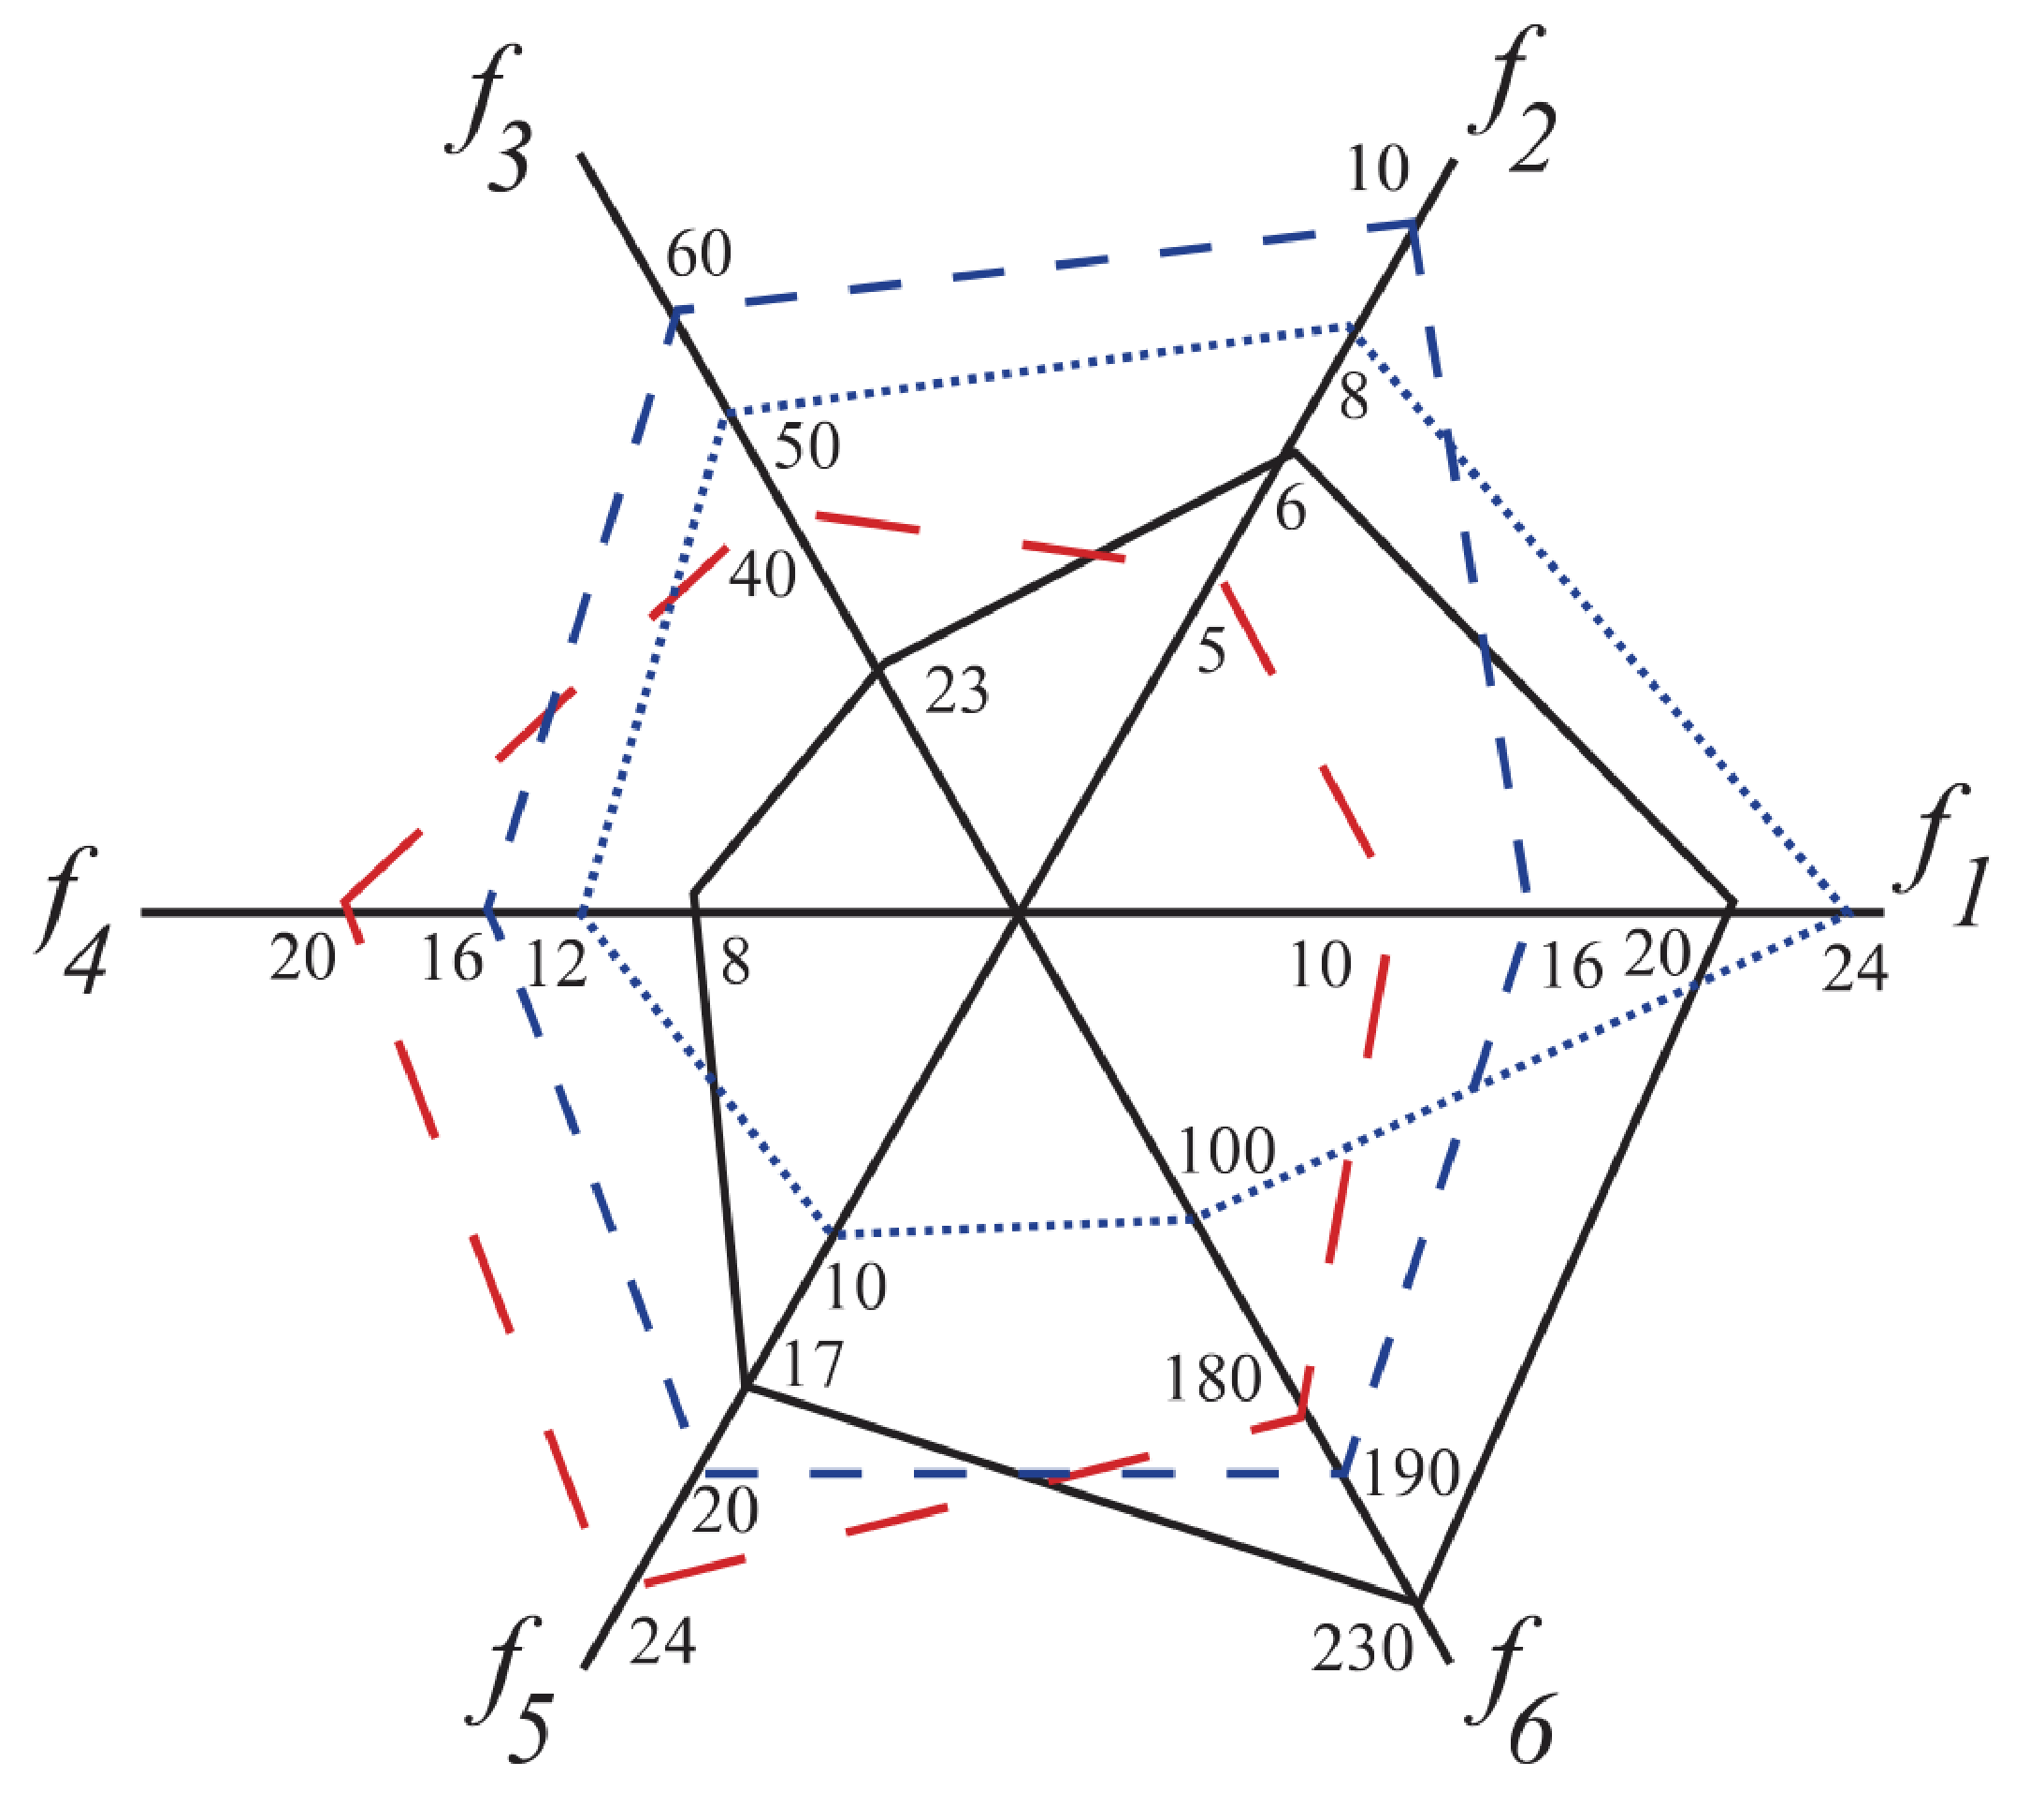
\includegraphics[width=0.45\columnwidth]{img/dp/fundamentaldefinitions/chart1}
	\end{center}
\end{enumerate}

\subsection{Decision-makers or stakeholders}
\label{subsec:decisionmakersdef}

A decision-maker is whoever takes part in a decision. The subjects who do not directly contribute to a decision, but play a role in it with their preferences are often denoted as stakeholders.

$D$ is a finite set which includes all stakeholders. They (directly or indirectly) set the value of the decision variables $x$
\begin{itemize}
	\item independently
	$$ X = X^{(1)} \times \dots \times X^{(d)} $$
	
	\item cooperatively
	$$ X = X^{(1)} \cap \dots \cap X^{(d)} $$
\end{itemize}

\subsection{Preference relation}
\label{subsec:prefreltiondef}

For each decision-maker, there is the need to distinguish \textit{which impact is preferred}, i.e., preferring $f \in F$ to $f' \in F$ means \textit{considering acceptable the replacement of $f'$ with $f$}. This corresponds to establishing a relation between pairs of impacts.

$\Pi: D \rightarrow 2^{F \times F}$ associates each decision-maker $d \in D$ to a subset of impact pairs that represents a binary relation $\Pi (d)$ on $F$.

Subset $\Pi(d) \in 2^{F \times F} \Leftrightarrow \Pi(d) \subseteq F \times F$ collects the specific pairs of impacts between which $d$ has a weak preference
$$ \Pi_d = \{(f, f') \in F \times F \mid d \text{ weakly prefers } f \text{ to } f'\} $$

\begin{definition}
	A \textbf{weak preference} is when $d$ accepts to exchange $f'$ for $f$ (not strict)
	$$ f \wpref{d} f' \Leftrightarrow (f, f') \in \Pi_d$$
\end{definition} 

In the finite case, a preference relation can be represented by
\begin{enumerate}
	\item an \textbf{incidence matrix} (rows and columns are impacts, the ones are preferences)
	\begin{center}
		\begin{tabular}{@{}l|rrrrr@{}}
			\toprule
			& $f$ & $f'$ & $f''$ & $f'''$ & $f''''$ \\
			\midrule
			$f$   & 1 &  0 & 1 & 1 & 1 \\
			$f'$  & 0 & 1 & 1 & 1 & 1 \\
			$f''$  & 0 &  0 & 1 &  1 & 1 \\
			$f'''$ & 0 &  0 & 0 & 1 & 0 \\
			$f''''$ & 0 & 0 & 1 & 1 & 1 \\
			\bottomrule
		\end{tabular}
	\end{center}
	
	\item a \textbf{preference graph}
	\begin{center}
		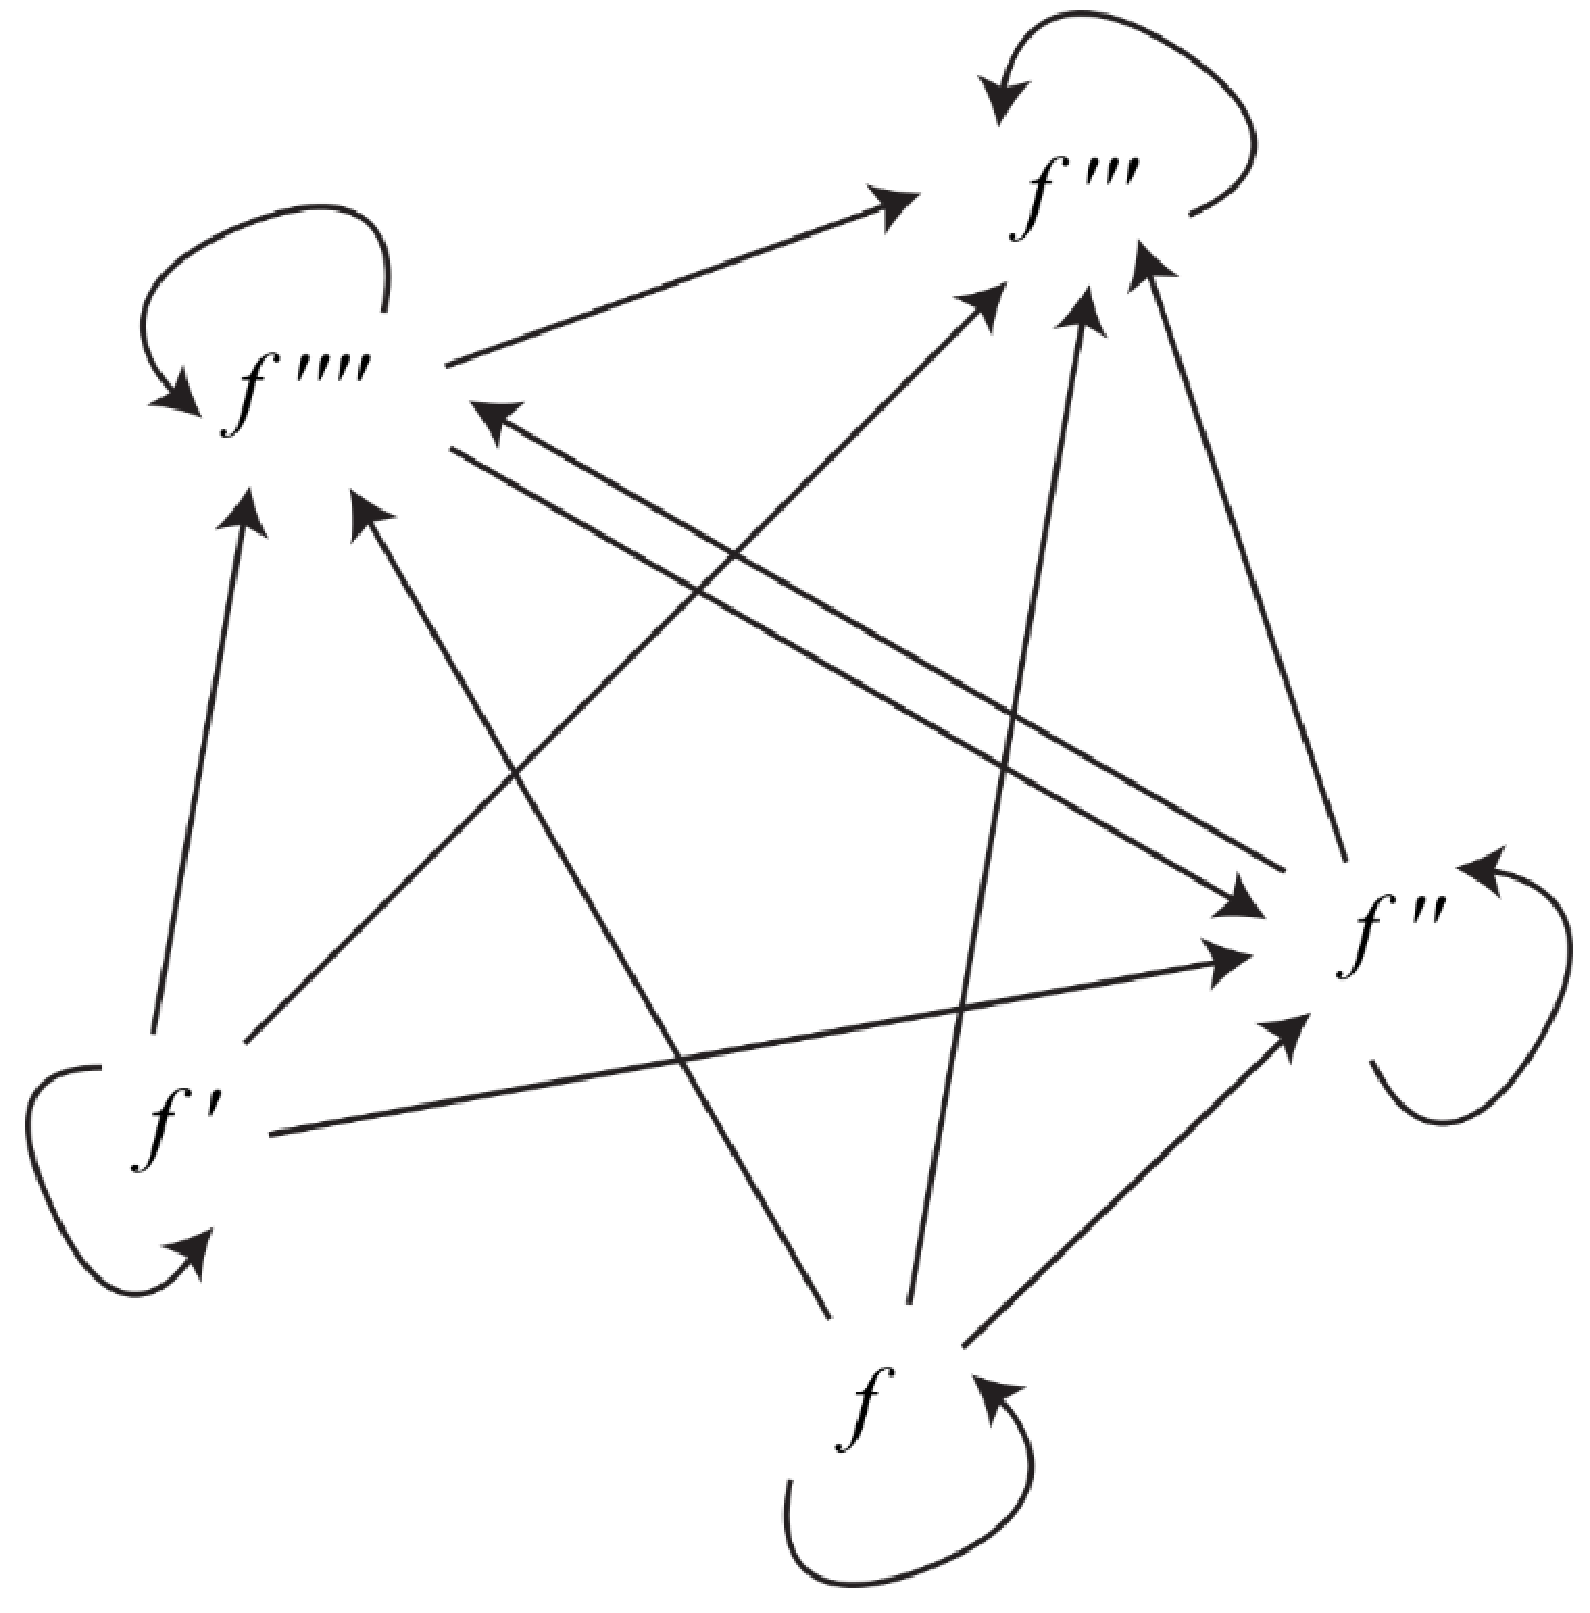
\includegraphics[width=0.45\columnwidth]{img/dp/fundamentaldefinitions/graph1}
	\end{center}
\end{enumerate}

\subsubsection{Derived relations}
\label{subsubsec:derivedrelations}

From the weak preference relation, one can derive
\begin{itemize}
	\item \textbf{Indifference} relation ($\indiff{\Pi} = \Pi \cap \Pi^{-1}$), definition:
	$$ f \sim f' \Leftrightarrow f \wpref{} f' \text{ and } f' \wpref{} f $$
	\textit{The decision-maker accepts the exchange in both directions}
	
	\item \textbf{Strict preference} relation ($\spref{\Pi} = \Pi \setminus \Pi^{-1}$), definition
	$$ f \prec f' \Leftrightarrow f \wpref{} f' \text{ and } f' \not \wpref{} f $$
	\textit{The decision-maker accepts the exchange only in the given direction}
	
	\item \textbf{Incomparability} relation ($\inc{\Pi} = \bar \Pi \cap \bar \Pi^{-1}$), definition
	$$ f \bowtie f' \Leftrightarrow f \not \wpref{} f' \text{ and } f' \not \wpref{} f $$
	\textit{The decision-maker rejects the exchange in both directions} (the decision-maker is not indifferent between the impacts, but is unable or unwilling to chose between them, refusing both exchanges)
\end{itemize}

\subsection{Property of binary relations}
\label{subsec:propertybinrel}

Not all binary relations express reasonable preference relations for a decision-maker. In principle, the preference relation should be 
\begin{itemize}
	\item \textit{Realistic}, it models correctly the aims of the decision-maker
	
	\item \textit{Effective}, it allows algorithms that yield a satisfactory choice
\end{itemize}

The two are, surprisingly, often conflicting.

Some preference relations enjoy some other special properties
\begin{itemize}
	\item \textbf{Reflexivity}: $f \wpref{} f$, $\forall f \in F$; it would be meaningless to consider a decision-maker unable to compare an impact to itself
	
	\item \textbf{Antisymmetry:} if $f \wpref{} f'$ and $f' \wpref{} f$, then $f = f'$ for all $f, f' \in F$; two impacts are indifferent only if they are identical
	
	\item \textbf{Completeness:} if $f \not \wpref{} f'$, then $f' \wpref{} f$ for all $f, f' \in F$; it requires the decision-maker to be able to always sort the impacts, though allowing ties; this excludes incomparability
	
	\item \textbf{Transitivity:} if $f \wpref{} f'$ and $f' \wpref{} f''$, then $f \wpref{} f''$, for all $f, f', f'' \in F$; discussed later
\end{itemize}

While building the model, we must investigate whether they hold or not, because they could be
\begin{itemize}
	\item useful to simplify the computation
	
	\item but unrealistic for the given problem
\end{itemize}

\paragraph{Main kinds of preference relation} Combining these properties, we can identify different kinds of preferences:
\begin{itemize}
	\item A \textbf{preorder} enjoys reflexivity and transitivity
	
	\item a \textbf{partial order} enjoys reflexivity, transitivity and antisymmetry; example: subset inclusion
	
	\item a \textbf{weak order} enjoys reflexivity, transitivity and completeness; example: rankings in sport
	
	\item a \textbf{total order} enjoys reflexivity, transitivity, antisymmetry and completeness; example: number sizes
\end{itemize}

\paragraph{Conceptual problems on transitivity} Transitivity is the most common assumption for a preference relation, and is often interpreted as an equivalent for rationality.

Rational decision-makers are transitive, humans are not. There are two main approaches to deal with this point:
\begin{enumerate}
	\item \textit{humans should be transitive}, i.e., use thought experiments to show the evil consequences of giving up transitivity
	
	\item \textit{let humans be non-transitive}, i.e., appeal to practical and thought experiments and adopt weaker models of rationality
\end{enumerate}

%End of L3

	
	\part{Basic Decision Models}
	
	% !TeX spellcheck = en_US
\chapter{Structured preferences}
\label{ch:structpref}

How can we use the concept introduced to choose a solution for a decision problem? 

We'll assume: 
\begin{itemize}
	\item A simple preference relation $\Pi$
	
	\item A certain environment $|\Omega| = 1 \implies f(x, \bar \omega)$ reduces to $f(x)$
	
	\item A single decision-maker $|D| = 1 \implies \Pi_d$ reduces to $\Pi$
\end{itemize}

Single scenario and single decision-maker. Also, the preference relation of the decision-maker will be a weak order (reflexive, transitive and complete).

The first two conditions allow a well-posed definition of solutions that can be justifiably selected and the third allows the choice of a single solution.

\section{Dominance relation}
\label{sec:dominancerel}

The preference relation between impacts $(\Pi \subseteq F \times F)$ projects onto an \textbf{induced relation between solutions}. A solution \textit{dominates} another when the impact of the former is preferable to the impact of the latter.
$$ x \wpref{} x' \Leftrightarrow f(x) \wpref{} f(x') \quad \forall x, x' \in X $$

\begin{definition}
	We denote as \textbf{dominated solution} a solution $x \in X$ such that $\exists x' \in X : f(x') \prec f(x)$, \textbf{nondominated solution}. We denote as $X^\ast \subseteq X$ the set of \textbf{all nondominated solutions}.
\end{definition}

This implies a partition of the feasible region into
\begin{itemize}
	\item dominated solutions: $x \in X$ such that $\exists x' \in X: x' \prec x$
	
	\item nondominated solutions: the other ones
\end{itemize}

\textbf{Reflexivity} looks natural in a preference relation. When solving a decision problem, it is also rather natural to 
\begin{itemize}
	\item \textbf{exclude dominated solutions}, that is choose $x^\ast \in X^\ast$
	
	\item Choose an \textbf{arbitrary solution from a set of mutually indifferent ones}
\end{itemize}

But this conflicts with some possible situations: 
\begin{itemize}
	\item All solutions in a strict dominance circuit would be removed
	
	\item Two solutions might be indifferent with respect to a third one, but incomparable with each other
\end{itemize}

Transitivity solves both problems. \textbf{Preorders} are strong candidates to \textbf{be preference relations}.

\subsection{Decision-making on preorders}
\label{subsec:decisionmakingpreorders}

\begin{theo}
	If the preference relation $\Pi$ is a preorder, the induced dominance is a preorder. \\
\end{theo}

\begin{theo}
	If the preference relation $\Pi$ is a preorder (reflexive and transitive) and the solution set is finite and nonempty ($X \neq \emptyset$), the nondominated solution set $X^\ast$ is nonempty.
\end{theo}

This guarantees that decision problems admit reasonable solutions. In some cases, $X^\ast$ will contain a single solution, or several mutually indifferent, in other cases it will include incomparable solutions. Therefore, determining $X^\ast$ simplifies the problem, but doesn't solve it completely.

\begin{theo}
	If preference $\Pi$ is a preorder and $X^\ast$ is nonempty, the nondominated solutions partition into disjoint components
	\begin{itemize}
		\item they are mutually indifferent within each component
		
		\item they are mutually incomparable between different components
	\end{itemize}
	$\implies$ if there is only one component, the problem is solved (requires completeness).
\end{theo}

\subsubsection{Identification of the nondominated solutions}

If $X$ is a finite set, it's possible to build the \textbf{strict preference graph}, whose nodes correspond to solutions, while the arcs correspond to solution pairs whose impacts are related by a strict preference. In this graph there are no indifferent pairs. 

The nondominated solutions correspond to \textit{nodes with no ingoing arc} (from each node there's an arrow towards dominated solutions), to identify them it's sufficient to scan each node of the graph and search for nodes with zero indegree.

Let $O(\gamma)$ be the complexity of computing the preference between two given impacts (non necessarily constant, they must be computed and compared), then the overall complexity for the search is $O\left(\gamma |X|^2\right)$ (for each node, compare its impact to the one ov every other in time $\gamma$).

This obviously can't be applied to infinite sets and could be impractical even in the case of combinatorial sets.

\subsection{Decision-making on weak orders}
\label{subsec:decisionmakingweakorders}

\begin{theo}
	If preference $\Pi$ is a weak order (reflexive, transitive and complete), the induced dominance is a weak order. \\
\end{theo}

\begin{theo}
	If preference $\Pi$ is a weak order (reflexive, transitive and complete) and $X$ is finite and nonempty, nondominated solutions exist and are all mutually indifferent.
\end{theo}

This allows to choose any of such solutions as the overall solution of the problem. This is good, the aim is to "make the right choice". Weak orders allow to sort impact on a line, with possible ties, as if associating a degree to each impact.

\begin{definition}
	A \textbf{value function} is a function $v: F \rightarrow \R$ that associates a real value to each impact (also called \textit{utility functions in economics}). Function $v$ is \textbf{consistent} with preference relation $\Pi$ when 
	$$ f \wpref{} f' \Leftrightarrow v(f) \geq v(f'), \quad \forall f,f' \in F$$
	or, equivalently
	$$ \Pi = \left\{(f, f') \in F \times F \mid v(f) \geq v(f') \right\} $$
\end{definition}

This offers a compact way to represent preference relations, that is also good for computation
$$ \max_{x \in X} \left\{ v\left(f(x)\right) \right\}$$
if we have analytic expressions for $X$ and $v\left( f (\cdot)\right)$ and a solving algorithm.

Value functions are \textbf{not univocal} (infinite equivalent ones always exist).

If a preference relation admits a consistent value function, the derived relations of indifference and strict preference correspond to identity and strict inequality between the values of the value function. \\

\begin{theo}
	If a preference relation $\Pi$ admits a consistent value function $v(f)$, then $\Pi$ is a weak order (reflexive, transitive and complete).
\end{theo}

The proof is simple, the point is to show that the preference enjoys reflexivity (because $\Pi$ includes pair $(f,f)$ for all $f \in F$), transitivity (because for all triplets $f, f', f'' \in F$ such that relation $\Pi$ includes pairs $(f,f')$ and $(f', f'')$, it also includes pair $(f, f'')$), and completeness (because for each pair $(f, f')$ not included in $\Pi$, pair $(f',f)$ belongs to it).
%TODO: proof is missing, maybe do it?

In practice, we start from a preference relation, not from a value function, the inverse would be more useful (the decision problem could be reduced to a maximization of the value function), but it's not always true.

\subsubsection{Weak orders not reducible to a consistent value function}

\paragraph{Lexicographic order} The main example of weak order relation (actually, strong order relation), which doesn't admit a consistent value function. 

Considering the simplest two-dimensional case, with real components ($F = \R^2$), the preference relation is defined as
$$ 
\left[
\begin{array}{c}
	f_1 \\
	f_2
\end{array}
\right] \wpref{}  \left[
\begin{array}{c}
	f_1' \\
	f_2'
\end{array}
\right]
\Leftrightarrow f_1 < f_1' \text{ or } f_1 = f_1' \wedge f_2 \leq f_2'
$$
The decision-maker prefers the smaller impact of the first one, for any value of the second, preferring the smaller value of the second only in the case of a tie for the first.

It can be proven that this relation doesn't admit any consistent value function $v(f)$, that is assigning to each impact in $F$ a real value such that the preference between two impacts correspond to an inequality between the function values.

The intuitive reason is that no improvement of the second can compensate for a worsening, even very small, of the first.

\subsubsection{Multiplicity of the consistent value functions}
\label{subsubsec:multeplicityvalfunc}

The existence of a way to build a consistent value function does not imply its uniqueness. \\

\begin{theo}
	Given a value function $v: F \rightarrow \R$, consistent with a preference relation $\Pi$ on $F$, for any strictly increasing function $\phi: \R \rightarrow \R$ the composite function $\phi(v(\cdot))$ is also consistent with $\Pi$.
\end{theo}

If a weak order admits a consistent value function, it admits infinite equivalent ones, that associate to the same impacts different values, but sorted in the same way.

%P78 notes, section not part of the syllabus, read it and weep

\subsubsection{Weak order preference models}

\paragraph{Scalar impact} When the impact is one-dimensional, it's often easy (though not always) to turn it into a value function. E.g., if the impact
\begin{itemize}
	\item is a benefit, set $v(f) = f$
	
	\item is a cost, set $v(f) = -f$
	
	\item has a target value $\bar f$, set $v(f) = - \dist(f, \bar f)$
\end{itemize}

\paragraph{Borda count} In the finite case, every weak order admits a value function (Borda count)
$$ B(f) = |\left\{f' \in F \mid f \wpref{} f' \right\}|$$

Basically, the Borda count $B(f)$ is the number of solutions dominated by $f$.

\paragraph{Lexicographic order} If the indicators are all costs (or benefits) and are sorted by importance ($P = (\pi_1, \dots, \pi_p)$), the preference relation $\Pi$ is a total order
$$ f \wpref{} f' \Leftrightarrow f_{\pi_1} < f_{\pi_1}' \text{ or } \left\{
\begin{array}{c}
	f_{\pi_1} = f_{\pi_1}' \\
	f_{\pi_2} < f_{\pi_2}' 
\end{array}\right\} \text{ or } \dots \text{ or } \left\{\begin{array}{c}
f_{\pi_1} = f_{\pi_1}' \\
f_{\pi_2} = f_{\pi_2}'  \\
\dots  \\
f_{\pi_p} \leq f_{\pi_p}'
\end{array}\right\}
$$

It does not admit value functions, but can be solved as follows
\begin{itemize}
	\item find the whole set $X^\ast_{\pi_1}$ of optimal solutions for $\min_{x \in X} f_{\pi_1}(x)$
	
	\item find the whole set $X^\ast_{\pi_2}$ of optimal solutions for $\min_{x \in X^\ast_{\pi_1}} f_{\pi_2}(x)$
	
	\item \dots
	
	\item find a single optimal solution $x^\ast_{\pi_p}$ for $\min_{x \in X^\ast_{\pi_{p-1}}} f_{\pi_p}(x)$
\end{itemize}

\paragraph{Utopia point} This model of preference:
\begin{enumerate}
	\item Identifies an ideal impact $f^\ast$ independently optimizing each indicator
	$$ f_l^\ast = \min_{x \in X} f_l (x) $$
	and combining the optimal values in a vector $f^\ast = \left[f_1^\ast \dots f_p^\ast \right]^T$. Determining such value is a classical optimization problem, sometimes hard, but generally possible
	
	\item Finds a solution with impact having minimum "distance" from $f^\ast$
	$$ \min_{x \in X} \dist \left(f(x), f^\ast \right)$$
\end{enumerate}

Different definitions of distance imply different results (Manhattan distance, Euclidean distance, \dots; infinite different distances can be defined), and the choice is arbitrary. 

If the indicators are heterogeneous, the units of measure have an influence and conversion coefficients are required to standardize them. The choice of coefficient is complex and, at least partly, arbitrary.

%End L4

\section{Multi Attribute Utility Theory MAUT}
\label{sec:maut}

The \textbf{Multi Attribute Utility Theory (MAUT)} assumes that the preference relation of the decision-maker is a weak order, admitting a consistent value function, but the decision-maker is unable to make the value function explicit without help.

It poses the problem to derive from the preference relation $\Pi$ the consistent value function $u: F \rightarrow \R$. We'll denote $u(f)$ as \textit{utility function} (economical notation).

We assume: 
\begin{itemize}
	\item a preference relation $\Pi$ with a consistent utility function $u(f)$ 
	
	\item a certain environment: $|\Omega| = 1 \implies f(x, \bar \omega)$ reduces to $f(x)$
	
	\item a single decision maker: $|D| = 1 \implies \Pi_d$ reduces to $\Pi$
\end{itemize}

And we know the preference $\Pi$, but not the utility function $u(f)$. \textit{How to build it?}

Specific models of preference have specific applications, \textit{case by case, they might work or not}. We want a \textbf{general way to derive $u(f)$ from $\Pi$}
\begin{enumerate}
	\item Introduce a graphical tool (indifference map)
	
	\item Turn the graph into a function, with a complex error-prone process 
	
	\item Define a special case with a simpler process (additive value functions)
	
	\item Characterize the preference relations falling within the special case
\end{enumerate}


\subsection{Indifference Curves}
\label{subsec:indifferencecurves}

\begin{definition}
	Given an impact set $F$ in the space of the indicators $\R^p$ and a preference relation $\Pi$ which is a weak order, we denote as \textbf{indifference curve} every subset of impacts that are reciprocally different.
\end{definition}

An indifference curve is a set $I \subseteq F$ of \textbf{reciprocally indifferent impacts}. They always enjoy the following properties: 
\begin{itemize}
	\item The \textbf{curves covers} $F$: every impact belongs to a curve, due to the completeness of the relation
	
	\item Any two indifference curves $I$ and $I'$ have \textbf{empty intersection} (transitivity would merge them)
	
	\item The weak order on impacts maps onto a \textbf{total order on curves (antisymmetry)}; there are no incomparable impacts and all indifferent impacts belong to the same curve, so impacts on different curves are linked by strict preference
\end{itemize}

Usually, technical assumptions are made:
\begin{itemize}
	\item \textbf{Continuity} implies that the curves are \textit{regular mathematical objects} and not completely general set of points
	
	\item The utility function $u(f)$ has a \textbf{continuous infinity of values} $c \in \R$ 
	
	\item Each indifference curve is expressed in \textbf{implicit form}
	$$ u(f) = c $$
	
	\item When the implicit form $u(f) = c$ can be turned into an \textbf{explicit form}
	$$ f_l = f_l \left(c, f_1, \dots, f_{l-1}, f_{l+1}, \dots , f_p\right) $$
	an indifference curve is a \textbf{hypersurface of $p-1$ dimensions in $\R^p$} (when $p = 2$, it's a line in the plane)
\end{itemize}

If a value function is known, the family of all indifference curves admits an analytic representation in the indicator space $F$ through the equation $u(f) = c$, where $c$ is a constant parameter that identifies each single curve. This corresponds to an analytic representation of the solution space $X$ through the parametric equation $u(f(x)) = c$.

\subsubsection{Indifference curves and utility function (Indifference map)}

If a preference relation admits a consistent value function, it admits infinitely many (as seen in \ref{subsubsec:multeplicityvalfunc}); the indifference curves of such functions, however, are always the same. 

The correspondence between preference relations and indifference curves is one-to-one, the one between preference relations and value functions is one-to-many.

Given a weak order preference relation $\Pi$ on $F$, its \textbf{indifference map} $\I_\Pi$ is the ordered family of indifference curves covering $F$. The correspondence between $\Pi$ and $\I_\Pi$ is one to one
\begin{itemize}
	\item $\Pi$ identifies all groups of indifferent impacts (curves) and their order
	
	\item $\I_\Pi$ identifies the preference between all pairs of impacts
\end{itemize}

The indifference map $\I_\Pi$ corresponds to infinite utility functions $u(f)$.

\subsection{Determining the utility function}
\label{subsec:detutility}

Given a preference relation $\Pi$ on $F$: 
\begin{enumerate}
	\item Extract a sample $\tilde F$ from $F$
	
	\item Ask the decision-maker to 
	\begin{itemize}
		\item sort the sampled impacts
		
		\item Identify their equivalence classes
	\end{itemize}
	
	\item Draw an interpolating curve for each equivalence class 
	
	\item Guess a parametric utility function family from their shape 
	$$ u = u_\alpha (f) \text{ with } \alpha = \left[\alpha_1 \dots \alpha_p \right]^T $$
	
	\item Each pair of indifferent impacts implies an equation on $\alpha$
	$$ f \sim f' \Leftrightarrow u(f(\alpha)) = u(f'(\alpha)) $$
	
	\item Add a normalization condition to select one of the equivalent utilities
	
	\item Make consistency checks by comparing other pairs of impacts; if they fail, go back to 4 and change the parametric utility
\end{enumerate}

The process is, in general, very complex and error prone
\begin{itemize}
	\item Large samples are costly
	
	\item The sample must include at least $p-1$ pairs of indifferent impacts found by trial and error
	
	\item Small samples ($\approx p$) lead to likely incorrect curves; if the samples is too large, the workload for the decision maker becomes huge (if $k$ different values for each indicator leads to $k^p$ different impacts to evaluate)
	
	\item Numerical errors over many equations combine in cascade
	
	\item Mutually dependent pairs are useless
	
	\item High dimensional spaces make it hard to draw curves and guess $u_\alpha$
\end{itemize}

Some properties (not guaranteed) which allow to make easier estimates, helping to draw curves and guessing $u(f)$:
\begin{itemize}
	\item \textbf{Invertibility:} $u(f)= c$ can be solver with respect to each $f_l$
	\begin{itemize}
		\item always verified when the indicators are costs or benefits
		
		\item basically, when we can get each indicator $f_l$ from the function $u(f)$ (analytically, the function can be inverted)
	\end{itemize}
	Under this assumption, an indifference curve $u(f) = c$ can be written in explicit form as $f_l = f_l (c, f_1, \dots, f_p)$
	
	\item \textbf{Monotony:} strictly decreasing or increasing difference curves (\textit{an increase in one is balanced by a decrease in another})
	\begin{itemize}
		\item always verified when the indicators are all costs or benefits
	\end{itemize}
	In order to compensate for the variations of an indicator, the other ones must vary in a well-determined direction
	
	\item \textbf{Convexity} or \textbf{concavity} ("law of diminishing marginal utility"): 
	\begin{itemize}
		\item costs lead to concave curves, benefits to convex ones
	\end{itemize}
	The indifference curves compensate for the increase of an indicator by a certain amount with variations of the other ones that increase (or decrease) with the value of the first indicator; basically, if a resource (indicator) is scarce, increasing it brings a large utility, compensated by a strong decrease of other resources, if a resource is abundant the same increase brings a small utility, compensated bt a weak decrease of other resources (this is the case of convex curves, they would be concave in the case of indicators expressing cost)
\end{itemize}

\subsection{Additive utility functions (game changer)}
\label{subsec:additiveutil}

\begin{definition}
	We denote a utility function as \textbf{additive} when it can be expressed as the sum of functions of the single indicators:
	$$ u(f_1, \dots, f_p) = \sum_{l = 1}^p u_l (f_l) $$
\end{definition}

It's a specific case that brings many simplifications:
\begin{itemize}
	\item Ask different decision-makers for each indicator $f_l$ (\textit{split the work})
	
	\item Ask decision-makers with experience in the sector (\textit{more reliable})
	
	\item Compare scalar values $f_l$ instead of vectors $f$ (\textit{easier and better})
	
	\item Build functions $u_l (f_l)$ with one argument (\textit{easier and better})
\end{itemize}

Since a utility function has infinitely many forms, \textbf{a nonadditive function can have an additive equivalent form}, but \textit{that is not guaranteed, how can we know?}

Example (Cobb-Douglas functions):
$$ u(f) = \prod_{l=1}^{p} f_l^{\alpha_l} \text{ is equivalent to } u'(f) = \log u (f) = \sum_{l = 1}^p \alpha_l f_l $$

If the utility function is additive, the problem of estimating it can be reduced to the estimation of $p$ single-variable functions, making the process easier.

\subsection{Preferential Independence}
\label{subsec:preferentialindependence}

How to know that $\Pi$ admits an additive consistent utility function? Given the set of attribute indices $P = \left\{1, \dots, p\right\}$, focus on subset $L \subset P$; we can write that
$$ f = \left[
\begin{array}{c}
	f_L \\
	f_{P\setminus L}
\end{array}
\right]$$
where $f_L$ and $f_{P\setminus L}$ are the subvectors of impact $f$ corresponding, respectively, to the indicators of $L$ and $P \setminus L$ (we just divided the whole thing in two parts).\\

\begin{definition}
	A proper subset of indicators $L$ is \textbf{preferentially independent} from the complementary subset $P \setminus L$ when, given two impacts with identical values of the indicators in $P \setminus L$, the preference relation between them does not depend on such values:
	$$ 
	\left[
	\begin{array}{c}
		f_L \\
		\phi 
	\end{array}
	\right]
	\wpref{}
	\left[
	\begin{array}{c}
		f_L' \\
		\phi 
	\end{array}
	\right]
	\Leftrightarrow
	\left[
	\begin{array}{c}
		f_L \\
		\psi
	\end{array}
	\right]
	\wpref{}
	\left[
	\begin{array}{c}
		f_Lì \\
		\psi
	\end{array}
	\right]
	$$
	for all subvectors $\phi$, $\psi$, $f_L$, $f_L'$ such that the four impacts are in $F$:
	$$ 
	\left[
	\begin{array}{c}
		f_L \\ \phi
	\end{array}
	\right],
	\left[
	\begin{array}{c}
		f_L' \\ \phi
	\end{array}
	\right],
	\left[
	\begin{array}{c}
		f_L \\ \psi
	\end{array}
	\right],
	\left[
	\begin{array}{c}
		f_L' \\ \psi
	\end{array}
	\right] \in F
	$$
\end{definition}

Preferences between values in $L$ do not depend on the values out of $L$. 

For example: a cost is preferentially independent from all other indicators (the lower the better), but this is not true for a thermostat, at a certain humidity a lower temperature is better, at other ones, a higher temperature might be better.

Preferential independence is \textbf{not symmetric}:
$$L \text{ independent from } P\setminus L \centernot \implies P \setminus L \text{ independent from } L $$

Preferential independence \textbf{on single indicators does not imply independence on larger subsets}: 
$$ \left\{l\right\} \text{ independent from } P \setminus \{l\}, \ \forall l \in P \centernot \implies L \text{ independent from } P \setminus L, \forall L \subseteq P $$

\subsubsection{Mutual preferential independence}

Preferential independence of relation $\Pi$ and additivity of function $u(f)$ are strictly connected, even if not rigorously equivalent. \\

\begin{definition}
	We say that a problem enjoys \textbf{mutual preferential independence} when every proper subset of indicators $L \subset P$ is independent from its complement $P \setminus L$.
\end{definition}

Mutual preferential independence is a necessary condition for additivity.

The above definition requires to check every nonempty proper subset $P \subset L$: 
\begin{itemize}
	\item $2^p - 2$ subsets
	
	\item infinite 4-tuples of subimpacts (to sample) for each subset \\
\end{itemize}

\begin{theo}
	Mutual preferential independence holds if and only if, given $\bar l \in P$, every pair $L = \left\{l, \bar l \right\}$ is preferentially independent from $P \setminus L$ for all $l \in P \setminus \{\bar l\}$
\end{theo}

We need to check only $p-1$ pairs (\textit{but single indicators are not enough}). \\

\begin{theo}
	If $\Pi$ admits a consistent additive utility function $u(f)$, then $\Pi$ enjoys mutual preferential independence.
\end{theo}

To verify this is enough to apply the definition (for a more detailed proof, p.92 of the notes).

The problem is that the opposite is needed, we can verify mutual preferential independence and not additivity, as the utility function is always unknown, we need a sufficient condition. \\

\begin{theo}
	A decision problem with $p \geq 3$ indicators enjoying mutual preferential independence admits an additive utility function $u(f)$.
\end{theo}

Unfortunately, when $p=2$, mutual preferential independence is necessary but not sufficient for additivity, as it reduces to checking each indicator with respect to the other one.

% End L4, p 93/94 of the notes

\subsection{Marginal rate of substitution MRS}
\label{subsec:mrs}

To summarize, we know the preference $\Pi$, not the utility function $u(f)$ and the general process to find it is complex and error-prone. For additive functions it's much simpler, but is $u(f)$ additive?
\begin{itemize}
	\item for $p \geq 3$, mutual preferential independence $\Leftrightarrow$ additivity
	\item for $p = 2$, mutual preferential independence $\impliedby$ additivity
\end{itemize}

The problem lies in how the indifference curves behave in $F$; the missing condition to guarantee additivity concerns the steepness of the indifference curve. We need a measure of steepness.

The behavior of a curve is described by the relation between $f_1$ and $f_2$: from $f$, vary $f_1$ and update $f_2$ so as to remain on the indifference curve. \\

\begin{definition}
	We denote as \textbf{marginal rate of substitution (MRS)} of $f_1$ with $f_2$ in a given impact $f$ the limit 
	$$ \lambda_{12} (f) = \lim_{\delta f_1 \rightarrow 0} - \frac{\delta f_2 (f, \delta f_1)}{\delta f_1} $$
	where $\delta f_2 (f, \delta f_1)$ is such that $f + \left[\begin{array}{c}
		\delta f_1 \\ \delta f_2 (f, \delta f_1)
	\end{array}\right] \sim f$
\end{definition}

In other words, the MRS is the limits, for infinitesimal variations of $f_1$, of the ration between the variations of $f_2$ and $f_1$ that produces impacts indifferent with respect to $f$. The sign of the limit is reversed because it's often negative (e.g. when the two indicators are both costs or benefits).

In problems with more than two indicators, a marginal rate of substitution os defined for each pair of indicators, and is computed assuming that all other indicators remain constant.

The definition assumes to start from an impact $f$, slightly modifying the value of indicator $f_1$ and determining the corresponding variation of $f_2$ that allows to stay on the initial indifference curve.

Assuming that the indifference curves are regular arcs and representing them in parametric form (two functions of parameter $\alpha$, continuous up to the first derivative): 
$$
\begin{cases}
	f_1 = f_1 (\alpha) \\ f_2 = f_2 (\alpha)
\end{cases}
$$

The variations $\delta f_1$ and $\delta f_2$ used in the definition of $\lambda_{12}(f)$ correspond to a variation $\delta \alpha$ of the parameter, guaranteeing that the impact remains on the indifference curve and allowing us to express the MRS as
$$ \lambda_{12} (f) ? \lim_{\delta f_1 \rightarrow 0} - \frac{\delta f_2 (f, \delta f_1)}{\delta f_1} = \lim_{\delta \alpha \rightarrow 0} - \frac{f_2 (\alpha + \delta \alpha) - f_2 (\alpha)}{f_1 (\alpha + \delta \alpha) - f_1 (\alpha)} = - \frac{\frac{df_2}{d\alpha}}{\frac{d f_1}{d \alpha}} $$

This form is useful to prove \textbf{reciprocity}:
$$ \lambda_{12} (f) = \frac{1}{\lambda_{21} (f)} $$

\paragraph{MRS and utility function} A second expression shows the relation between MRS and $u(f)$; by changing $\alpha$ we move along the indifference curve, but the utility function remains constant: $u(f(\alpha)) = c$ for all $\alpha$, therefore having a first derivative equal to zero with respect to $\alpha$:
$$ \frac{d u(f_1 (\alpha), f_2 (\alpha))}{d \alpha} = 0 \implies \frac{\partial u}{\partial f_1} \frac{d f_1}{d \alpha} + \frac{\partial u}{\partial f_2} \frac{d f_2}{d \alpha} = 0 \implies - \frac{\frac{df_2}{d\alpha}}{\frac{df_1}{d \alpha}} = \frac{\frac{\partial u}{\partial f_1}}{\frac{\partial u}{\partial f_2}} $$

And this implies that
$$ \lambda_{12} (f) = \frac{\frac{\partial u}{\partial f_1}}{\frac{\partial u}{\partial f_2}} $$

The MRS of $f_1$ with $f_2$ is the ratio of the partial derivatives of the utility function with respect to $f_1$ and $f_2$. If the utility depends strongly on $f_1$ and weakly on $f_2$, the MRS is large, i.e., a large variation of $f_2$ is required to compensate for a small variation of $f_1$.

This form also holds for $p \geq 3$ indicators, given that the rate of substitution is defined keeping all indicators constant, except for two.

\paragraph{MRS and indifference curves} If the indifference curves are invertible, each value of parameter $\alpha$ corresponds to a different value of $f_1$ and $f_2$, one can define  a function $\alpha = \alpha (f_1)$ which implies an explicit expression for the indifference curve: $f_2 = f_2 (\alpha (f_1))$. The first derivative of that expression is
$$ \frac{df_2}{df_1} = \frac{df_2}{d\alpha} \frac{d \alpha}{d_f1}  = \frac{\frac{df_2}{d\alpha}}{\frac{df_1}{d \alpha}} $$
From which
$$ \lambda_{12} (f) = - \frac{d f_2}{d f_1} $$

The MRS is the \textit{negative slope of the tangent to the indifference curve}; the steepness of the indifference curves, with a reverse sign.

In simple terms, the MRS is how much of $f_2$ are you willing to give away for a small increase of $f_1$.

\subsection{Additivity and MRS}
\label{subsec:additivityandMRS}

By combining two distinct values for $f_1$ ($f_1'$ and $f_1''$) and $f_2$ ($f_2'$ and $f_2''$) one can build four different impacts. In general, the  MRS in these four are fully independents, however, they can be related. \\

\begin{definition}
	We denote as \textbf{corresponding trade-off condition} the following property
	$$ \lambda_{12} (f_1', f_2') \lambda_{12} (f_1'', f_2'') = \lambda_{12} (f_1'', f_2') \lambda_{12} (f_1', f_2'') $$
	for every quadruplets of impacts $(f_1', f_2'), (f_1'', f_2''), (f_1'', f_2'),  (f_1', f_2'') \in F$.
\end{definition}

Some indifference maps enjoy such property, and it is \textbf{global}: it relates far away impacts.

The corresponding trade-off condition is easier to interpret if rewritten as
$$ 
\frac{\lambda_{12} (f_1', f_2')}{\lambda_{12} (f_1'', f_2')} = \frac{\lambda_{12} (f_1', f_2'')}{\lambda_{12} (f_1'', f_2'')}
\ \text{ or } \
\frac{\lambda_{12} (f_1', f_2')}{\lambda_{12} (f_1', f_2'')} = \frac{\lambda_{12} (f_1'', f_2')}{\lambda_{12} (f_1'', f_2'')}
$$

Basically, multiplying two MRSs on the diagonal of a rectangle (composed by 2 values for each of the 2 indicators) is the same as multiplying the two MRSs for the values on the opposite diagonal.

\begin{center}
	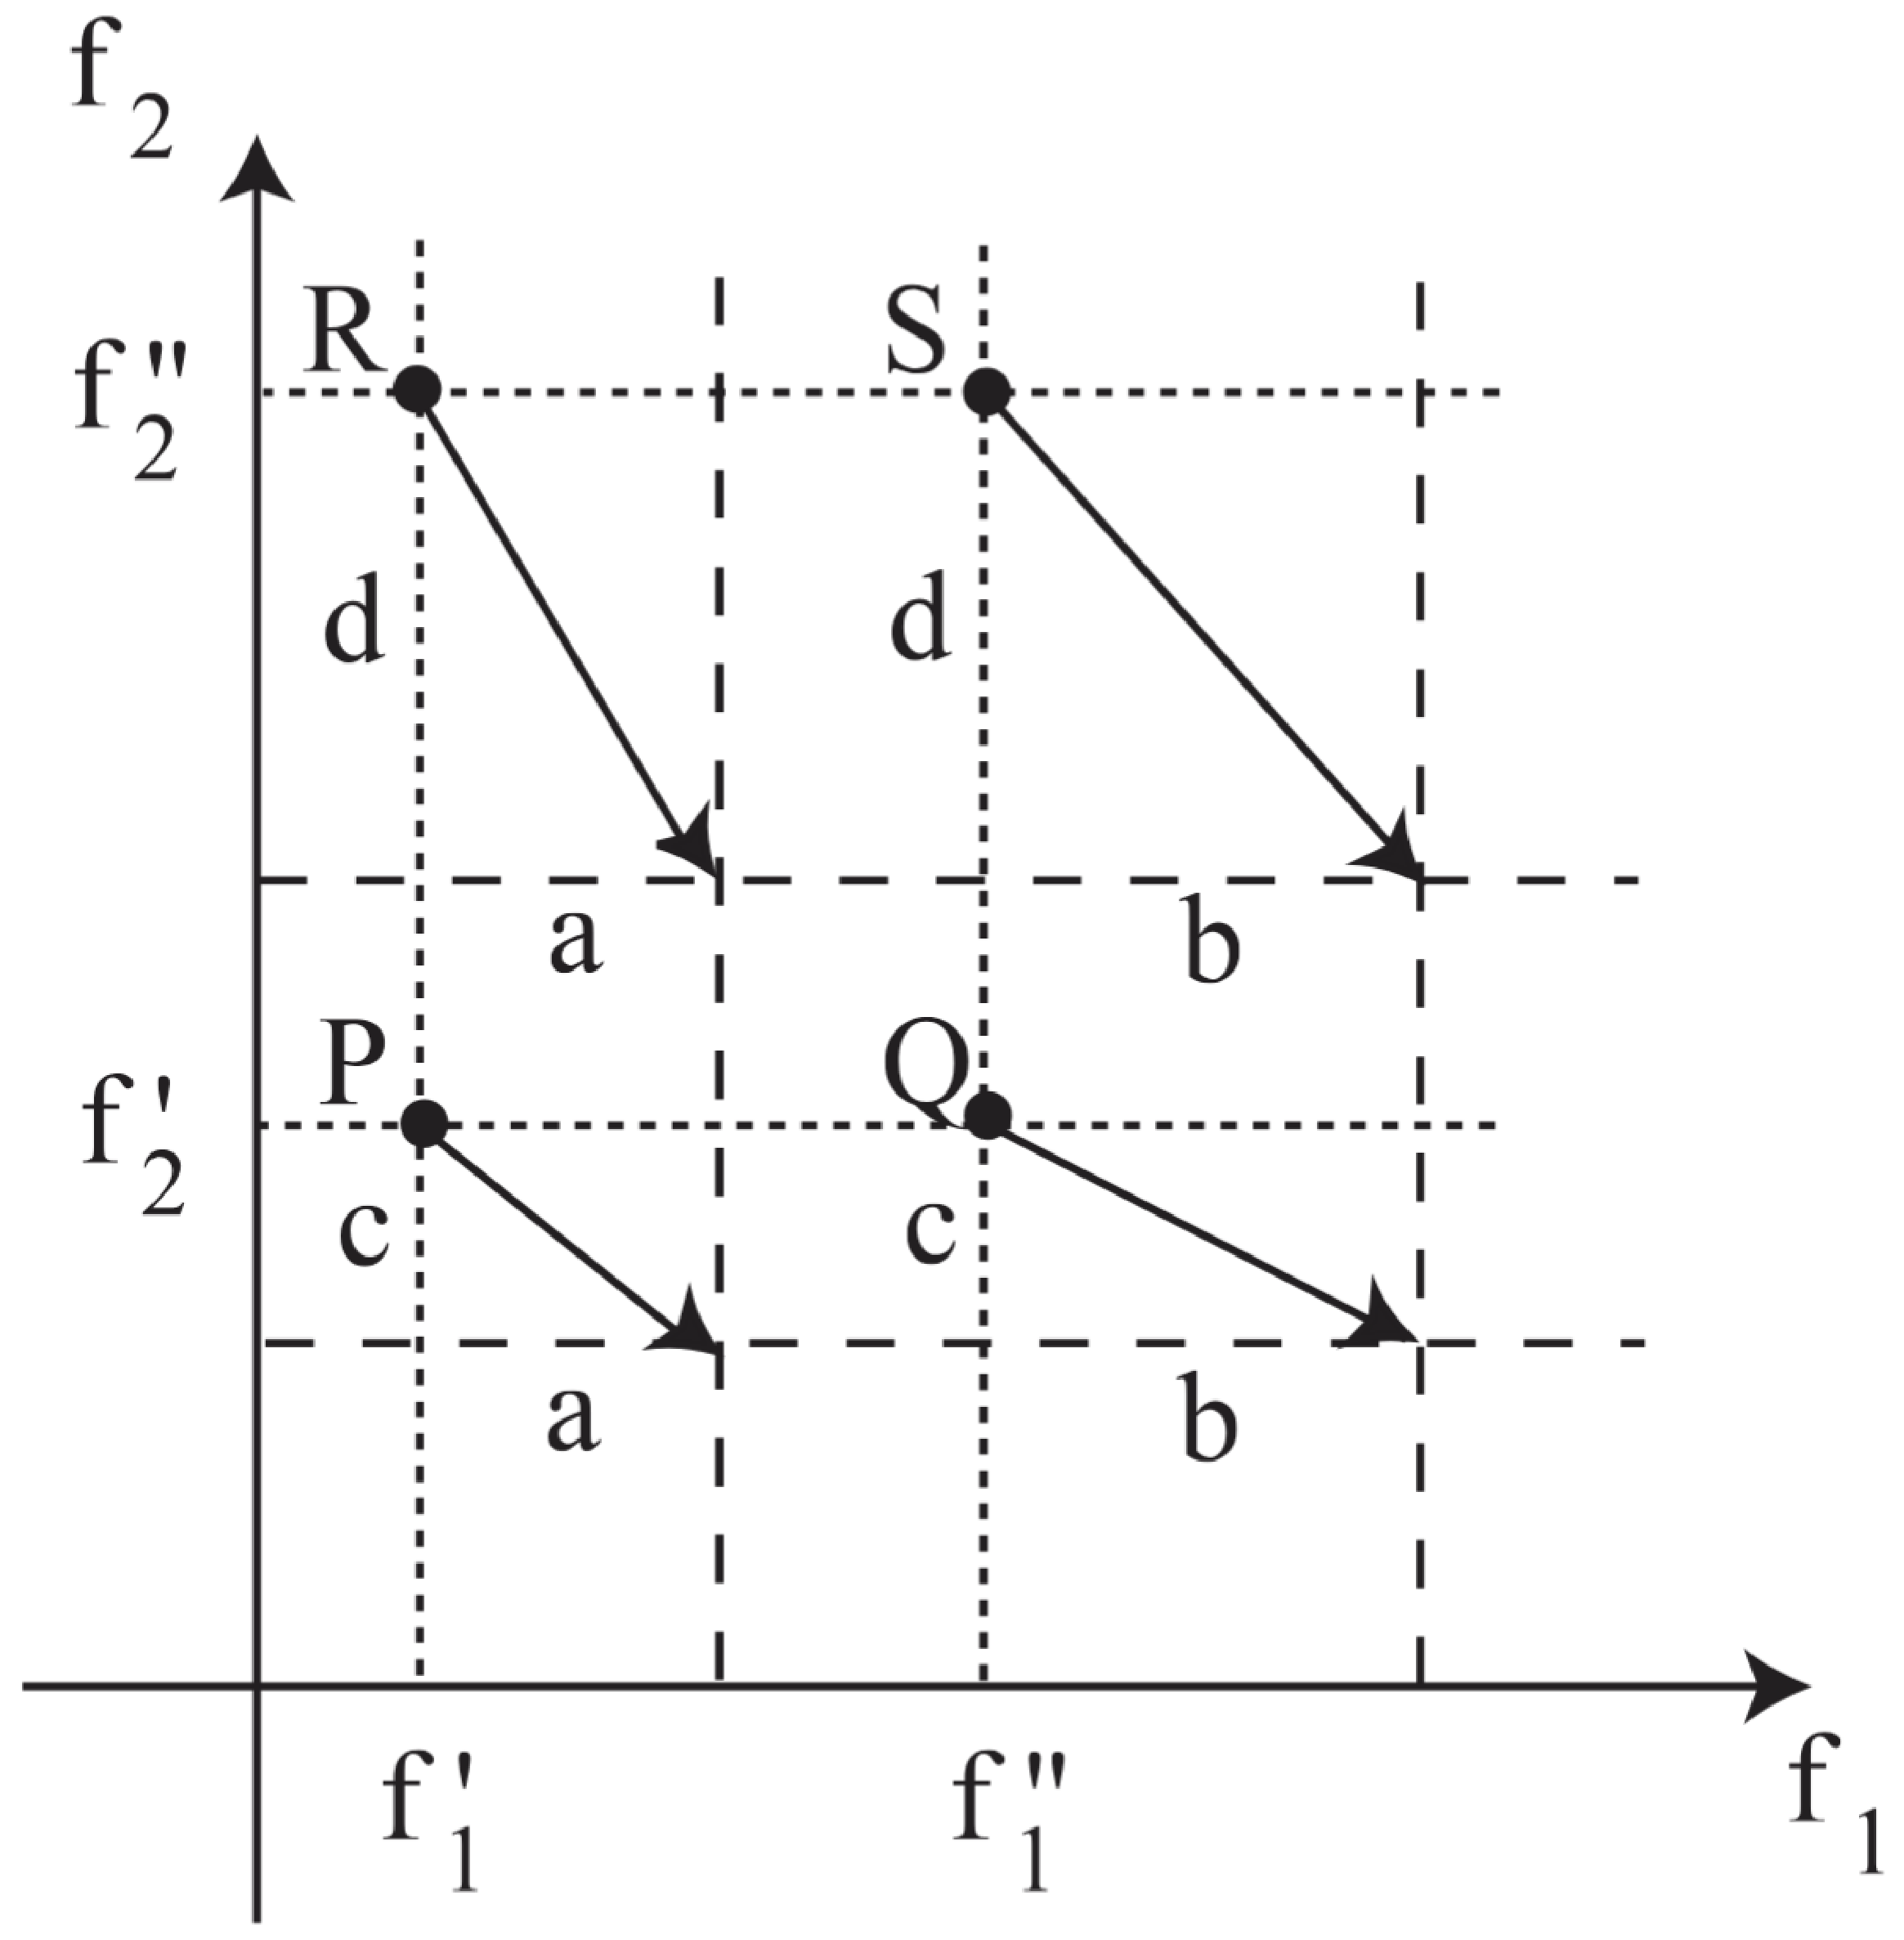
\includegraphics[width=0.45\columnwidth]{img/bdm/structpref/mrs1}
\end{center}
In the image it can be seen that in the four points $P$, $Q$, $R$ and $S$ the MRSs are, respectively, equal to $-a/c$, $-b/c$, $-a/d$, $-b/d$. The product of the rates in $P$ and $S$ is $ab/cd$, and it coincides with the product of the rates in $Q$ and $R$.

The ratio of $\lambda$ between points with the same abscissa does not depend on the abscissa. In other words, even if the MRS is nonuniform, it changes by the same factor moving between the same coordinates. \\

\begin{theo}
	A preference relation $\Pi$ admits an additive utility function $u(f)$ if and only if it enjoys both
	\begin{enumerate}
		\item mutual preferential independence
		
		\item the corresponding trade-off condition
	\end{enumerate}
\end{theo}

The "only-if part" it's easy to prove, the "if" was needed in order to assume additivity.

\begin{proof}
	Once again, it's a matter of applying the definition:
	$$ \lambda_{12} (f_1', f_2') \lambda_{12} (f_1'', f_2'') = \frac{\frac{\partial u}{\partial f_1'}}{\frac{\partial u}{\partial f_2'}} \frac{\frac{\partial u}{\partial f_1''}}{\frac{\partial u}{\partial f_2''}} $$
	Since $u(f_1, f_2) = u_1(f_1) + u_2(f_2)$:
	$$ \lambda_{12} (f_1', f_2') \lambda_{12} (f_1'', f_2'') = \frac{\frac{\partial u}{\partial f_1'}}{\frac{\partial u}{\partial f_2'}} \cdot \frac{\frac{\partial u}{\partial f_1''}}{\frac{\partial u}{\partial f_2''}} 
	= 
	\frac{\frac{\partial u}{\partial f_1'}}{\frac{\partial u}{\partial f_2''}} \frac{\frac{\partial u}{\partial f_1''}}{\frac{\partial u}{\partial f_2'}}
	$$
	and getting back to function $u(f_1, f_2)$:
	$$ 
	\lambda_{12} (f_1', f_2') \lambda_{12} (f_1'', f_2'') = \frac{\frac{\partial u}{\partial f_1'}}{\frac{\partial u}{\partial f_2''}} \frac{\frac{\partial u}{\partial f_1''}}{\frac{\partial u}{\partial f_2'}}
	= \lambda_{12} (f_1', f_2'') \lambda_{12} (f_1'', f_2')
	$$
\end{proof}

The corresponding trade-off condition is thus necessary for additivity (also sufficient, under suitable conditions).

To assume additivity: 
\begin{itemize}
	\item When $p \geq 3$, check mutual preferential independence for $p-1$ indicator pairs
	
	\item When $p=2$ check
	\begin{itemize}
		\item independence for the single indicators
		
		\item the corresponding trade-off condition
	\end{itemize}
\end{itemize}

\subsection{Building an additive utility function}
\label{subsec:buildingadditive}

The expression for an additive utility function
$$ u(f) = \sum_{l = 1}^p u_l (f_l) $$
assumes the same measure unit for all $u_l$ function. In practice, different fields use different units, therefore:
\begin{enumerate}
	\item Adopt normalized utilities: pure numbers $\tilde u_l (f_l)$ instead of $u_l (f_l)$, usually within the interval $[0,1]$
	
	\item Introduce weights $w_l$ to combine them
	$$ u(f) = \sum_{l = 1}^p w_l \tilde u_l (f_l) $$
\end{enumerate}

Intuitively, we are splitting the task into "rescaling" indicators into utilities, removing nonlinearities, and "combining" heterogeneous utilities into a single one.

The normalized utility expression is a \textbf{linear} and \textbf{convex} combination: 
\begin{itemize}
	\item \textbf{Conic:} all coefficients are nonnegative ($w_l \geq 0$ for all $l \in P$)
	
	\item \textbf{Affine:} the coefficients have unitary sum ($\sum_{l = 1}^p w_l = 1$)
\end{itemize}

\subsubsection{The bisection method}

Building a utility function for a one-dimensional impact ($F \subseteq \R$) is much easier than for a multidimensional one, it only takes comparing pairs of numbers and wondering which one of the two is better. 

However, the function we want to build must respect a condition stronger than just sorting all impacts, we want to measure the strength of relative preference: nearly indifferent impacts should have similar utility values and impacts well distinguished from a preferential point of view should have very different utility values.

The bisection methods builds such function with a dichotomic approach. For example, to build the normalized utility $\tilde u_C(C)$ for the daily calorie intake $C$, given $F_C = [0, 10000]$, interview an expert about a specific individual
\begin{enumerate}
	\item Ask the expert for the worst values in $F_C$ (for example, $C_1^\dag \leq 1000$ and $C_2^\dag \geq 6000$) and set $\tilde u_C (C) = 0$ for such values
	
	\item Ask the expert for the best values in $F_C$ (for example, $2200 \leq C^\ast \leq 2600$) and set $\tilde u_T (22) = 1$ for such values
	
	\item Ask the expert for values of exactly intermediate utility between $T^\dag$ and $T^\ast$ (for example, $C = 1800$ and $3000$) and set $\tilde u_C (C) = 1/2$
	
	\item Go on, asking for values of intermediate utility between the fixed ones and set $\tilde u_T$ accordingly
	
	\item Guess an interpolating function
\end{enumerate}

When the indicator represents a cost or benefit, sometimes it's possible to assume the utility proportional to the indicator $f_l$. We can easily generate a normalized utility function:
$$ \tilde u_l (f_l) = \frac{f_l - \min_{x \in X} f_l (x)}{\max_{x \in X} f_l (x) - \min_{x \in X} f_l (x)} $$
Switch them for costs.

If $\min_{x \in X} f_l (x)$ or $\max_{x \in X} f_l (x)$ are unknown or hard to compute, an underestimate and overestimate can be used instead, yielding a normalized utility function, different from above mentioned one. This can lead to a "compression" of the value range if the estimates are loose (it's not using the whole interval $[0,1]$).

\subsection{Determining the weights}
\label{subsec:detweights}

We still need to determine the weights with which to combine the components of the additive utility function. This requires to identify a sufficient number of pairs of indifferent impacts, equaling the utilities of the two impacts imposes a constraint on the weights of $w_l$, allowing us to find a single solution, with enough constraints (linear equation system).

As in the general case, $p-1$ independent pairs of indifferent impacts are needed: 
\begin{itemize}
	\item The equations are linear in $w$ 
	$$ f \sim f' \Leftrightarrow \tilde u (f) = \tilde u (f') \Leftrightarrow \sum_{l = 1}^p \tilde u_l (f_l) w_l = \sum_{l = 1}^p \tilde u_l (f_l') w_l$$
	
	\item The normalization condition imposes convexity 
	$$ \sum_{l = 1}^p w_l = 1$$
\end{itemize}

This process works correctly in the ideal case, but if indifference is imprecise, the pairs five wrong weights. The solution is to build a complete pairwise comparison of all indicators and analyze its consistency.

\subsubsection{The pairwise comparison matrix}

Select a pair of indifferent impacts $(f, f')$ with:
\begin{itemize}
	\item Different values for $f_l$ and $f_m$
	
	\item Identical values for all other indicators, $f_n = f_n'$ for all $n \in P \setminus \{l, m\}$
\end{itemize}

The equation reduces to 
$$ w_l \tilde u_l (f_l) + w_m \tilde u_m (f_m) = w_l \tilde u_l (f_l') + w_m \tilde u_m (f_m') $$
That simply becomes
$$ \tilde \lambda_{lm} = \frac{w_l}{w_m} = - \frac{\tilde u_m (f_m') - \tilde u_m (f_m)}{\tilde u_l (f_l') - \tilde u_l (f_l)} $$

\begin{definition}
	We denote as \textbf{pairwise comparison matrix} $\tilde \Lambda = \{\tilde \lambda_{lm}\}$ the matrix reporting all rates of substitution between the normalized utilities.
\end{definition}

It contains all the weight ratios
$$ \tilde \Lambda = \left\{\frac{w_l}{w_m}\right\} $$
expressing the relative weights between the single normalized utilities, that is, indicators (once nonlinearities and units of measure are removed).

A correct pairwise comparison matrix $\tilde \Lambda$ enjoys the following properties:
\begin{itemize}
	\item \textbf{Positivity:} $\tilde \lambda_{lm} > 0$ for all $l,m \in P$
	
	\item \textbf{Reciprocity:} $\tilde \lambda_{lm} = \frac{1}{\tilde \lambda_{ml}}$ for all $l,m \in P$
	
	\item \textbf{Consistency:} $\tilde \lambda_{ln} = \tilde{ \lambda_{lm}} \tilde \lambda_{mn}$ for all $l,m,n \in P$
\end{itemize}
We can check these properties on $\tilde \Lambda$ to be sure that $u(f)$ makes sense.

\subsection{The process in summary}
\label{subsec:detfunctionsummary}

In summary, the process to determine the utility function is composed of the following steps: 
\begin{enumerate}
	\item Interview the decision-maker in order to understand whether mutual preferential independence holds (ask to compare different pairs of indicators with the complementary subset)
	
	\item In the positive case, focus on each attribute, fixing the other ones to any value, and build a single-variable component of the utility function with a method respecting the entity of the relative preference gaps
	
	\item Determine the weights with which to combine such functions, sampling impacts until a sufficient number of pairs of indifferent impacts has been found
	
	\item Check \textit{a posteriori} that the obtained utility function is valid, testing it on impacts not used before
\end{enumerate}

In any moment, it can be necessary to go back to correct the single components of the utility or even rejecting the additivity assumption, in which case the whole process is invalidated.

%End L6, p115 notes, skipping excercises
	% !TeX spellcheck = en_US
\chapter{Mathematical Programing}
\label{ch:mathprog}

This chapter will deal with the simplest class of decision problems We assume:
\begin{itemize}
	\item A preference relation $\Pi$ with a known consistent utility function $u(f)$
	$$ \exists u: F \rightarrow \R : \Pi = \left\{(f,f') \in F \times F \mid u(f) \geq u(f')\right\} $$
	
	\item A certain environment: $|\Omega| = 1 \implies f(x, \bar \omega)$ reduces to $f(x)$; a single scenario, the impact $f$ depends only on the alternative $x$
	
	\item A single decision-maker: $|D| = 1 \implies \Pi_d$ reduces to $\Pi$
\end{itemize}

This class of problems reduces the decision problem to classical optimization: 
$$ \max_{x \in X} u(f) $$
We'll discuss a solving technique that is very general but complex and inefficient.

This class of problems is mainly treated in mathematical literature, where preference is expressed as a cost function, so the most common form is
$$ \min_{x \in X} f(x) $$
where $f(x)$  replaces $-u(f(x))$ (not the original $f$).

We also assume regularity for the objective and feasible region:
\begin{itemize}
	\item $f(x) \in C^1 (X)$; the cost function is continuous with its first derivative
	
	\item $X = \left\{x \in \R^n \mid g_j (x) \leq 0, \ j = 1, \dots, m\right\}$ with $g_j (x) \in C^1 (X)$; the solution set $X$ can be described through a finite system of inequalities, where the constraint functions $g_j(x)$ are real-valued continuous functions with a continuous first derivative in the feasible solution set of the problem
\end{itemize}

These are very general assumptions. This class of problem (with assumptions more or less strict with respect to the continuity of functions) are denoted under the label of \textbf{Mathematical Programming} problems, describing both preference and feasible region through real-valued functions allows to apply mathematical analysis to these decision problems.

\section{Basic concepts}
\label{sec:mathbasic}

\begin{definition}
	Given a set $X \subseteq \R^n$ and a function $f: X \rightarrow \R$ we denote as \textbf{global optimum point} a point $x^\circ \in X$ such that
	$$ f\left(x^\circ \right) \leq f(x) \quad \forall x \in X $$
\end{definition}

\begin{definition}
	Given a set $X \subseteq \R^n$ and a function $f: X \rightarrow \R$, we denote as \textbf{local optimum point} a point $x^\ast \in X$ such that 
	$$ \exists \epsilon > 0 : f\left(x^\ast\right) \leq f(x), \quad \forall x \in X \cap \U_{x^\ast, \epsilon} $$
	where
	$$ \U_{x^\ast, \epsilon} = \left\{x \in \R^n \mid \| x - x^\ast \| < \epsilon \right\} $$
	is a neighborhood of $x^\ast$ of width $\epsilon$ ($\|x - x^\ast \|$ is the norm of vector $x - x^\ast$).
\end{definition}

It can easily be seen that a global optimum is, by definition, also a local optimum:
$$ X^\circ \subseteq X^\ast $$

There is no process to find $X^\circ$ or $X^\ast$ directly, so we want to search the conditions necessary for local optimality. These conditions aim to identify points "candidate" to being local optimum, weakening twice our request:
$$ 
\begin{array}{c c c c c}
	\text{Global optimum} & \implies & \text{Local optimum} & \implies & \text{KKT conditions} \\
	$X^\circ$ & \subseteq & X^\ast & \subseteq & X^{KKT} 
\end{array}
$$
The conditions are known as \textbf{Karush-Kuhn-Tucker conditions}, from the names of their discoverers.

After finding the "weakened" set, we enumerate $X^{KKT}$ exhaustively to find $X^\circ$. 

The KKT conditions identify candidate points as follows: 
\begin{enumerate}
	\item Lay out the conditions as a system of equalities and inequalities
	
	\item Solve the system, finding $X^{KKT}$
	
	\item Evaluate every point in $X^{KKT}$, keeping only the best ones (which will compose $X^\circ$)
\end{enumerate}

The method requires $X^{KKT}$ to be a finite set, or at least a set which can be analytically describes, in order to determine $X^\circ$.

The basic tool will be linear approximation in small neighborhoods (hence the false positives).

\subsection{Taylor's series expansion}
\label{subsec:taylor}

Every sufficiently regular function (i.e., continuous function with continuous derivatives up to a suitable order $k$) can be locally approximated with a polynomial of degree $k$. \\

\begin{theo}
	Let $f \in C^k \left(\U_{\tilde x, \epsilon}\right)$ be a function of a real variable $x \in \R$. For all $x \in \U_{\tilde x, \epsilon}$, Taylor's series expansion holds: 
	$$ f(x) = \sum_{i = 0}^k \frac{f^{(i)} (\tilde x)}{i!} (x - \tilde x)^i $$ 
	$$ \text{with } f^{(0)}  = f, \quad f^{(i)} = \frac{d^i f}{dx^i} \quad \forall i \in \N^+, \text{ and } \lim_{x \rightarrow \tilde x} \frac{R_k (x - \tilde x)}{\|x - \tilde x\|} = 0$$
\end{theo}

Any regular function can be locally approximated in $\tilde x$ by its tangent line, terms with exponents higher than 1 improve the approximation (which we'll not consider). Any function regular up to the first order ($f: \R \rightarrow \R$ and $f \in C^1 (\U_{\tilde x, \epsilon})$) admits a linear approximation
$$ f(x) = f(\tilde x) +  f'(\tilde x) (x - \tilde x)  + R_1 (|x - \tilde x|)$$
which can be generalized to multiple-variable functions ($x \in \R^n$) by 
$$ f(x) = f(\tilde x) + \left(\nabla f(\tilde x)\right)^T (x  - \tilde x) + R_1 (\|x - \tilde x\|) $$
where 
$$ \lim_{x \rightarrow \tilde x} \frac{R_1 \left(\|x - \tilde x\|\right)}{\|x - \tilde x\|} = 0$$
and $\nabla f(x)$ is the gradient vector
$$ 
\nabla f(x) = \left[\begin{array}{c}
	\frac{\partial f}{\partial x_1} \\ \dots \\ \frac{\partial f}{\partial x_n}
\end{array}\right]
$$
It's the direction of quickest increase for $f(\cdot)$.

\subsection{Arcs}
\label{subsec:arcs}

$\R^n$ offers many ways to move away from $\tilde x$.\\

\begin{definition}
	Given a point $\tilde x \in \R^n$, an \textbf{arc} in $\tilde x$ is a parametric curve $\xi: \R^+ \rightarrow \R^n$, that is $\xi (\alpha) = \left[\begin{array}{c}
		\xi_1 (\alpha) \\ \dots \\ \xi_n (\alpha)
	\end{array}\right]$, such that $\xi (0) = \tilde x$ and $\xi_1 (\alpha) \in C^1 (\R^+)$.
\end{definition}

Basically, a function that starts at $\tilde x$ (since $\xi (0) = \tilde x$) and then gets further from it, with each component continuously differentiable for $\alpha > 0$. \\

\begin{definition}
	An arc $\xi (\alpha)$ is \textbf{feasible} for a given region $X \subseteq \R^n$ when the curve remains in $X$ for small $\alpha$
	$$ \exists \bar \alpha_f > 0 : \xi (\alpha) \in X, \quad \forall \alpha \in [0; \bar \alpha_f) $$
\end{definition}

Given a region $X$ (our function), we can travel "a little" (a small enough interval, as defined) along the arc without leaving $X$. \\

\begin{definition}
	An arc $\xi (\alpha)$ is \textbf{improving} for a given function $f:X \rightarrow \R$ when $f$ is strictly better in $\xi (\alpha)$ than in $\tilde x$ for all small positive $\alpha$
	$$ \exists \bar \alpha_i > 0 : f\left(\xi(\alpha)\right) < f (\tilde x), \quad \forall \alpha \in (0; \bar \alpha_i) $$
\end{definition}

Along the curve, but close enough to $\tilde x$, the value of the function $f$ is strictly better than in $\tilde x$.

\section{Necessary conditions for local optimality}
\label{sec:necforlocal}

\begin{theo}
	If $\tilde x \in X \subseteq \R^n$ (a point in a region), $f(\cdot) \in C^1 (X)$ (continuously differentiable function) and $\xi (\alpha)$ is an arc in $\tilde x$, feasible for $X$ and improving for $f(\cdot)$, then $\tilde x$ is not locally optimal for $f(\cdot)$ in $X$.
\end{theo}

If a feasible improving arc in $\tilde x$ exists, then $\tilde x$ can't be a local optima; no improving arc can exist ar a local optima.

\begin{proof}
	By assumption, for suitable values $\bar \alpha_f > 0$ and $\bar \alpha_i > 0$, we have:
	\begin{itemize}
		\item $\xi (\alpha)$ feasible: $\xi (\alpha) \in X$ for all $\alpha \in [0, \bar \alpha_f)$
		
		\item $\xi (\alpha)$ improving: $f(\xi(\alpha))  < f(\tilde x)$ for all $\alpha \in (0, \bar \alpha_i)$
	\end{itemize}
	
	Since $\xi (\alpha)$ is a continuous arc 
	$$ \lim_{\alpha \rightarrow 0} \xi(\alpha) = \tilde x \Leftrightarrow \forall \epsilon > 0, \ \exists \bar \alpha_\epsilon  : \| \xi(\alpha)  - \tilde x \| < \epsilon, \ \forall \alpha \in (0, \bar \alpha_\epsilon ) $$
	that is, $\xi (\alpha) \in \U_{\tilde x, \epsilon}$, $\forall \alpha \in (0, \bar \alpha_\epsilon )$.
	
	Now $\alpha = \frac{1}{2} \min (\bar \alpha_f, \bar \alpha_i \bar \alpha_\epsilon )$ satisfies all three conditions: 
	\begin{itemize}
		\item $\alpha < \bar \alpha_f \implies \xi(\alpha) \in X$
		
		\item $\alpha < \bar \alpha_i \implies f(\xi(\alpha)) < f(\tilde x)$
		
		\item $\alpha < \bar \alpha_\epsilon \implies \xi(\alpha) \in \U_{x^\ast, \epsilon}$
	\end{itemize}
	But this contradicts local optimality
	$$ f(x) \geq f(\tilde x), \quad \forall x \in \U_{\tilde x, \epsilon}  \cap X $$
\end{proof}

\subsection{A filtering approach}
\label{subsec:filteringapproach}

This suggests an approach to find candidate points: remove from $X$ all the points that are provably nonoptimal:
\begin{enumerate}
	\item Consider all feasible points as candidates: $C := X$
	
	\item Scan the set of candidate points $C$
	
	\item For each candidate point $\tilde x$, scan all feasible arcs
	
	\item For each arc $d$ feasible in $\tilde x$, check whether the arc is improving for $f(\cdot)$: if it is, remove $\tilde x$ from the candidate set
	
	\item In the end, scan the remaining candidate points, keeping only the best ones
\end{enumerate}

The pseudo-code of which being:
\begin{myalgo}{0.85}
	$X^{KKT} := X$; \\
	\tcp{(continuous set for $x$)}
	\For{\texttt{each} $x \in X^{KKT}$}{
		\tcp{(continuous set for $\xi$, interval for $\alpha$)}
		\For{\texttt{each} arc $\xi(\alpha)$ in $x$ feasible for $X$}{
			\tcp{(interval for $\alpha$)}
			\If{$\xi(\alpha)$ is improving in $x$ for $f(\cdot)$}{
				$X^{KKT}:=X^{KKT} \setminus \{x\}$; \\
			}
		}
	}
	\Return{$X^{KKT}$;}
\end{myalgo}

Problem: the set of feasible points and directions is, generally, infinite. We can replace the infinite loops with more efficient analytic conditions, all based on first-order approximations. \\

\begin{definition}
	We denote as \textbf{tangent direction} of an arc $\xi (\alpha)$ feasible in $\tilde x$ the vector composed of the first derivatives of the components $\xi_i$ with respect to parameter $\alpha$, evaluated in the starting point of the arc
	$$ p_\xi = \left[\begin{array}{c}
		\xi_1'(0) \\ \dots \\ \xi_n'(0) \\
	\end{array}\right]$$
\end{definition}

Straight lines $\xi (\alpha) = \tilde x + \alpha d$ have tangent direction $d$ (\textit{arcs generalize directions}).

Example: the arc in $\tilde x = (2,0)$
$$ \xi (\alpha) = \left[\begin{array}{c}
	2 \cos \alpha \\ 2 \sin \alpha 
\end{array}\right] $$
describes the circumference with center in the origin and radius 2. Its tangent direction is 
$$ p_\xi = \left[\begin{array}{c}
	-2 \sin 0 \\ 2 \cos 0
\end{array} \right] = \left[ \begin{array}{c}
0 \\ 2
\end{array}\right] $$

\begin{theo}
	If $x^\ast$ is locally optimal in $X$ for $f(\cdot)$ and $\xi (\alpha)$ is a feasible arc in $x^\ast$ for $X$, then 
	$$ \nabla f (\tilde x)^T p_\xi \geq 0 $$
\end{theo}

\begin{proof}
	If $\xi (\alpha)$ is a feasible arc, there exists a coefficient $\bar \alpha$ such that $\xi (\alpha) \in X$ for all $\alpha \in [0;\bar \alpha)$ (remains in $X$ for a small $\alpha$) and since $x^\ast$ is a local optima, for small $\alpha$ it holds that $f(\xi (\alpha)) \geq f(x^\ast)$. 
	
	Apply Taylor's expansion to $f(\xi (\alpha))$ in $\alpha = 0$
	\begin{align*}
		f(\xi (\alpha)) & \geq f(x^\ast) \implies \\
		\implies \cancel{f(\xi (0))} + \left \frac{df}{d\alpha} \right|_{\alpha = 0} \alpha + R_1 \left(\|\xi(\alpha) - \xi (0) \|\right) & \geq \cancel{f(x^\ast)} \implies  \\
		\implies \left(\nabla f(x^\ast)\right)^T  p_\xi + \frac{R_1 \left(\| \xi (\alpha)  - \xi (0) \| \right)}{\alpha} & \geq 0 \\
	\end{align*}
	
	If $\alpha$ converges to 0, by continuity the inequality is preserved
	$$ \lim_{\alpha \rightarrow 0} \left( \left(\nabla f(\tilde x)\right)^T p_\xi + \frac{R_1 \left( \xi (\alpha) - \xi (0)\right)}{\| \xi (\alpha) - \xi (0) \|} \frac{\| \xi (\alpha) - \xi (0) \|}{\alpha}\right) \geq 0 \implies $$
	$$ \implies \left(\nabla f(\tilde x)\right)^T p_\xi \geq 0 $$
\end{proof}

Example: 
\begin{align*}
	\min f(x) & = x_2 \\ g_1 (x) & = x_1^2 + x_2^2 \ \leq 4
\end{align*}
with $\nabla f^T = [0 \ 1]$
\begin{itemize}
	\item Arc $\xi (\alpha) = \tilde x + \alpha [1 \ -1]^T$ is improving in $\tilde x = (-2, 0)$: therefore $\tilde x$ is not locally optimal
	$$ \nabla f (-2, 0)^T p_\xi = [0 \ 1] \cdot [1 \ -1]^T = -1 < 0 $$
	
	\item Arc $\xi (\alpha) = \tilde x + \alpha[1 \ 1]^T$ is nonimproving in $\tilde x = (0, -2)$: $\tilde x$ could be locally optimal (remains candidate until disproval)
	$$ \nabla f(0, -2)^T p_\xi = [0 \ 1] \cdot [1 \ 1]^T = 1 \geq 0 $$ 
\end{itemize}

%I don't get the "intuitive" reason this is true, to me it's just a formula

The earlier code can be simplified (possibly missing some removals) to
\begin{myalgo}{0.85}
	$X^{KKT} := X$; \\
	\tcp{(continuous set for $x$)}
	\For{\texttt{each} $x \in X^{KKT}$}{
		\tcp{(continuous set for $\xi$, interval for $\alpha$)}
		\For{\texttt{each} arc $\xi(\alpha)$ in $x$ feasible for $X$}{
			\tcp{($\xi (\alpha)$ is improving in $x$ for $f(\cdot)$)}
			\If{{\color{red} $\nabla f(\tilde x)^T p_\xi < 0$}}{
				$X^{KKT}:=X^{KKT} \setminus \{x\}$; \\
			}
		}
	}
	\Return{$X^{KKT}$;}
\end{myalgo}

\subsection{Feasibility condition}
\label{subsec:feasibilitycondition}

Given the analytic description of the feasible region
$$ X = \left\{x \in \R^n \mid g_j (x) \leq 0 \text{ for } j = 1, \dots, m \right\}$$
we approximate each function $g_j(\cdot)$ with Taylor's expansion.

However, feasibility differs from improvement in two regards: 
\begin{itemize}
	\item It involves many inequalities, instead of a single objective
	
	\item It requires weak conditions, instead of a strict one \\
\end{itemize}

\begin{definition}
	We denote as \textbf{active constraint} in a point $\tilde x \in X$ any constraint $g_j (x) \leq 0$ such that $g_j (\tilde x) = 0$. We'll indicate by $J_a (x) = \left\{j \in \{1, \dots, m\}: g_j (x) = 0\right\}$ the set of indices of the active constraints.
\end{definition}

Basically, the constraints exactly equal to zero when considered in point $\tilde x$, and $J_a$ is the set of indices for which this condition holds.

Given point $\tilde x$ we partition the constraints into two classes
\begin{enumerate}
	\item The \textbf{active constraints} ($J_a (\tilde x)$) are exactly satisfied: $g_j (\tilde x) = 0$
	
	\item The nonactive constraints are largely satisfied: $g_j (\tilde x) < 0$
\end{enumerate}

Example: 
\begin{align*}
	\min f(x) & = (x_1 - 1)^2 + x_2 \\
	g_1 (x) & = -x_1^2 - x_2^2 + 4 \leq 0 \\
	g_2 (x) & = x_1 - 3/2 \leq 0
\end{align*}

Active constraints: 
\begin{itemize}
	\item for $x = (-2,-2)$, no active constraints: $J_a (-2, -2) = \emptyset$
	
	\item for $x = (3/2, 0)$, one active constraint: $J_a (3/2, 0) = \{2\}$
	
	\item for $x = (3/2, \sqrt{7}/2)$, two active constraints: $J_a (3/2, \sqrt{7}/2) = \{1,2\}$ \\
\end{itemize}

\begin{theo}
	If $\xi (\alpha)$ is a feasible arc in $\tilde x \in$ for $X$, $p_\xi$ its tangent vector. Then
	$$ \nabla g_j (\tilde x)^T p_\xi \leq 0, \quad \forall j \in J_a (\tilde x) $$
\end{theo}
\begin{proof}
	If $\xi (\alpha)$ is an arc feasible in $\tilde x$, there exists a coefficient $\bar \alpha$ such that
	$$ g_j (\xi (\alpha)) \leq 0, \quad \forall \alpha \in [0; \bar \alpha) \text{ and } j = 1, \dots, m $$
	that is
	\begin{align*}
		g_j (\xi (\alpha)) & = g_j (\xi(0)) + \left \frac{dg_j}{d \alpha}\right|_{0} \alpha + R_1 (\|\xi(\alpha) - \xi(0) \|) = \\
		& = g_j (\tilde x) + \alpha (\nabla g_j(\tilde x))^T p_\xi + R_1 (\| \xi(\alpha) - \xi (0)\|) \leq 0
	\end{align*}
	
	The inequality is obvious for all constraints not active in $\tilde x$ and the other two terms converge to zero as $\alpha \rightarrow 0$. Therefore, by continuity, when $\alpha$ is sufficiently small, they cannot reverse the inequality. 
	
	For the constraints which are active in $\tilde x$, on the contrary, the inequality introduces a strict condition, in fact, for such constraints $g_j(\tilde x) = 0$ so that
	$$ g_j (\xi (\alpha)) = \alpha (\nabla g_j (\tilde x))^T p_\xi + R_1 (\|\xi (\alpha) - \xi (0) \|) \leq 0 $$
	Dividing both terms by $\alpha$ and considering the limit, by continuity the thesis follows
	$$ \lim_{\alpha \rightarrow 0} \left[(\nabla g_j (\tilde x))^T p_\xi + \frac{R_1 (\| \xi (\alpha) - \xi (0) \|)}{\| \xi(\alpha) - \xi (0) \|} \frac{\| \xi (\alpha) - \xi (0) \|}{\alpha} \right] = (\Delta g_j (\tilde x))^T p_\xi \leq 0$$
\end{proof}

Special case: equality constraints $h_i (x) = 0$ are always active and can be treated as pairs of active inequalities: $h_i (x) \leq 0$ and $-h_i (x) \leq 0$
$$
\begin{cases}
	\nabla h_i (\tilde x)^T p_\xi & \leq 0 \\
	- \nabla h_i (\tilde x)^T p_\xi & \leq 0 \\
\end{cases}
\implies \nabla h_i (\tilde x)^T p_\xi = 0
$$

For any feasible arc $\xi (\alpha)$, vector $p_\xi$ satisfies the conditions above, but a vector $p$ that satisfies them is not always tangent to a feasible arc. Luckily, the problem concerns only some degenerate points.

\subsubsection{Regular points}

\begin{definition}
	We denote as \textbf{regular point} for a given system of constraints $g_j (x) \leq 0$a point in which all active constraint have linearly independent gradients (\textbf{constraint qualification} condition).
\end{definition}

In a regular point, the conditions on the gradients of the active constraints are not only necessary, but also sufficient to guarantee that there exists a feasible arc with the given tangent vector. \\

\begin{theo}
	If $\tilde x$ is a regular point, then $\nabla g_j (\tilde x)^T p \leq 0$ for all $j \in J_a (\tilde x)$ if and only if there exists an arc $\xi (\alpha)$ in $\tilde x$ feasible for $X$ with tangent direction $p_\xi = p$.
\end{theo}

The necessary conditions for feasibility are also sufficient in regular points. The analytical conditions on the gradients can be used to check feasibility in all regular points, nonregular points must be explicitly tested (candidates by default). \\

\begin{coro}
	Let $f \in C^1 (X)$, $\tilde x \in X$ be a regular and local optimum point and $p$ a vector such that
	$$ (\nabla g_j (\tilde x))^T p \leq 0, \quad \forall j \in J_a (\tilde x) $$
	Then 
	$$ (\nabla f(\tilde x))^T p \geq 0 $$
\end{coro}

The code now becomes:
\begin{myalgo}{0.85}
	$X^{KKT} := X \setminus$ NonRegular$(g, X)$; \\
	\tcp{(continuous set for $x$)}
	\For{\texttt{each} $x \in X^{KKT}$}{
		\tcp{(arc $\xi (\alpha)$ in $x$ feasible for $X$)}
		\For{\texttt{each} {\color{red} $p \in \R^n : \nabla g_j (x)^T p \leq 0$, $\forall j \in J_a (x)$}}{
			\tcp{($\xi (\alpha)$ is improving in $x$ for $f(\cdot)$)}
			\If{{\color{red} $\nabla f(\tilde x)^T p_\xi < 0$}}{
				$X^{KKT}:=X^{KKT} \setminus \{x\}$; \\
			}
		}
	}
	$X^{KKT} := X^{KKT} \cup $ NonRegular$(g,X)$; \\
	\Return{$X^{KKT}$;}
\end{myalgo}

%Should be end of L7, notes p128
	
	\part{Models with complex preferences}
	
	% !TeX spellcheck = en_US
\chapter{The Paretian preference}
\label{ch:paretian}

We now consider a more complex decision framework: still a single decision maker and a single scenario, but the preference relation is no longer a weak order described by a consistent value (or cost) function.

We assume: 
\begin{itemize}
	\item A preference relation $\Pi$ that is no longer a weak order
	
	\item A certain environment $|\Omega| = 1 \implies f(x, \bar \omega)$ reduces to $f(x)$
	
	\item A single decision-maker: $|D| = 1 \implies \Pi_d$ reduces to $\Pi$
\end{itemize}
If $\Pi$ is a preorder, we at least have nondominated solutions $X^\circ$ but possibly incomparable with each other. 

We want to make assumption on the structure of the preference relation (different assumptions will lead to different models); the first model proposed in history is the one proposed by \href{https://en.wikipedia.org/wiki/Vilfredo_Pareto}{\texttt{Vilfredo Pareto}}. \\

\begin{definition}
	We denote as \textbf{Paretian preference} the relation
	$$ \Pi = \left\{(f, f') \mid f_l \leq f_l' \text{ for each } l \in \{1, \dots, p\}\right\} $$
	that is
	$$ f \leq f' \Leftrightarrow f_l \leq f_l' \text{ for each } l \in \{1, \dots, p\} $$
\end{definition}

This assumes that each indicator represents a cost (easily extendable to the benefit and mixed cases). 

This models only allows to compare impacts with elements that dominate each other all in the same orientation; this \textbf{incomparable indicators assumption}, meaning that the decision-maker is unable to compare two impacts when different indicators give opposite suggestions. This can make the model unrealistic.

This model can seem not very useful to make an actual choice, as it ends with proposing several incomparable solutions, but in practice it's a useful starting point to further refine the preference relation.

\section{Properties of the Paretian preference}
\label{sec:paretoproperties}

\begin{theo}
	The Paretian preference relation is a partial order (reflexivity, antisymmetry and transitivity).
\end{theo}

\begin{proof}
	In fact, it is
	\begin{itemize}
		\item Reflexive: $f \wpref{} f$, for all $f \in F$
		\begin{align*}
			&f_l = f_l, \ \forall l \in \{1, \dots, p\}  \\
			\implies & f_l \leq f_l, \ \forall l \in \{1, \dots, p\}  \\
			\implies & f \wpref{} f
		\end{align*}
		
		\item Transitive: $f \wpref{} f'$ and $f' \wpref{} f'' \implies f \wpref{} f''$ for all $f, f', f'' \in F$
		$$
		\begin{cases}
			f \wpref{} f' \\
			f' \wpref{} f''
		\end{cases}
		\implies \begin{cases}
			f_l \leq f_l' & \forall l \in \{1, \dots, p\} \\
			f_l' \leq f_l'' & \forall l \in \{1, \dots, p\}
		\end{cases}
		\implies 
		$$
		$$ \implies f_l \leq f_l'', \ \forall l \in \{1, \dots, p\} \implies f \wpref{} f'' $$
		
		\item Antisymmetric: $f \wpref{} f'$ and $f' \wpref{} f \implies f = f'$ for all $f, f' \in F$
		$$ 
		\begin{cases}
			f \wpref{} f' \\
			f' \wpref{} f
		\end{cases}
		\implies \begin{cases}
			f_l \leq f_l' & \forall l \in \{1, \dots, p\} \\
			f_l' \leq f_l & \forall l \in \{1, \dots, p\}
		\end{cases}\implies 
		$$
		$$ \implies f_l = f_l', \ \forall l \in \{1, \dots, p\} \implies f = f' $$
	\end{itemize}
\end{proof}

This can appear as trivial, bu the translation from the relation on impacts ($\wpref{}$) to the relation of indicators ($\leq$) is allowed only by Pareto's definition.

In general, the Paretial preference relation is \textbf{not complete}.

\section{Paretian dominance}
\label{sec:paretiandom}

We can reformulate the concept of domination: a solution dominates another if and only if the impact of the former is strictly preferred to the impact of the latter. The preference is strict to avoid rejecting all indifferent solutions (they should not dominate each other).

In the Pareto case, dominance is expressed as follows
$$ x' \prec x \Leftrightarrow f(x') \prec f(x) \Leftrightarrow \begin{cases}
	f_l (x') \leq f_l (x), \ \forall l \in \{1, \dots, p \} \\
	\exists \bar l \in \{1, \dots, p\} : f_{\bar l} (x') < f_{\bar l} (x)
\end{cases}$$

allowing to split feasible solutions in two groups, one of which can be rejected in every reasonable decision.\\

\begin{definition}
	We denote as \textbf{dominated solution} every feasible solution $x \in X$ that admits another solution $x' \in X$ which dominates it: 
	$$ 
	\exists x' \in X, \ \bar l \in \{1, \dots , p \} : \begin{cases}
		f_l (x') \leq f_(x), \ \forall l \in \{1, \dots, p\} \\
		f_{\bar l} (x') < f_{\bar l} (x)
	\end{cases}
	$$
\end{definition}

\begin{definition}
	We denote as \textbf{Paretian solution} every feasible solution $x \in X$ such that no other solution $x'$ dominates it
	$$ \forall x' \in X, \ \exists \bar l \in \{1, \dots, p\} : f_{\bar l} (x) < f_{\bar l} (x') \text{ or } f(x') = f(x) $$
\end{definition}

\begin{definition}
	We denote as \textbf{Paretian region} $X^\circ$ the set of all paretian solutions.
\end{definition}

Unless for infinite chains, $X^\circ$ is nonempty and contains reciprocally incomparable solutions (or indifferent solutions that have the same impact). The aim is to enumerate $X^\circ$ and then ask the decision-maker.

The Paretian region corresponds to the set of globally optimal points in Mathematical Programming, with two differences, due to the incompleteness of the Paretian preference: 
\begin{enumerate}
	\item the Paretian solutions are not preferable to all other solutions, whereas the globally optimal points are
	
	\item the Paretian solutions are not reciprocally indifferent, whereas the globally optimal points are
\end{enumerate}

This means that is not enough to find a single globally optimal point and ignore the others as is Mathematical Programming, in the Paretian case it's appropriate to find all Paretian solutions.

\section{Identification of the Paretian region}
\label{sec:identifyparetianregion}

The fundamental problem now is how to determine the Paretian region. We'll look at different ways to obtain it which provide, in general, different results, due to the fact that they usually generate an underestimate (subset) or overestimate (superset) of $X^\circ$.

Some methods to enumerate the Paretian region:

\resizebox{\textwidth}{!}{
	\renewcommand{\arraystretch}{1.4}
	\begin{tabular}{L{3cm} | L{2cm} | L{4cm} | L{3.1cm}}
		\textbf{Method} & \textbf{Generality} & \textbf{Practical limits} & \textbf{Result provided} \\
		\hline
		definition & finite & slow for CO & exact \\
		
		inverse transformation & $p = 2$ & human intervention & exact \\
		
		KKT conditions & regular & solving a system & overestimate \\
		
		weighted sum & general & parametric problem (inefficient sampling) & underestimate (bad for large $p$) \\
		
		$\varepsilon$-constraint & general & parametric problem, usually NP-hard (inefficient sampling) & overestimate (refined by repetition) \\
	\end{tabular}
}

\subsection{Applying the definition}
\label{subsec:applyingdefinition}

In the finite case, $X^\circ$ can be found by pairwise comparisons, of course taking $\Theta\left(p|X|^2\right)$ time in the worst case. \textit{This can be huge in combinatorial problems, where $|X| \in \Theta\left(2^n\right)$}.

We can build the solution dominance graph, whose nodes correspond to solutions and whose arcs correspond to the dominance relation. The solutions are nodes with no outgoing arcs.

\section{Inverse transformation method}
\label{sec:invtransformation}

This method also consists in applying the definition, but can be used on continuous problems, provided that they can be graphically represented in the indicator space. In fact, the method consists in a graphical solution of the problem, and requires to:
\begin{itemize}
	\item Determine the inverse $\phi: F \rightarrow X$ of the transformation $f: X \rightarrow F$ (if not unique, compute all inverse functions)
	
	\item Build the image of $X$ in $F$ through the impact function $f(x)$ by drawing the constraints $g_j (x(f)) \leq 0$
	
	\item Find graphically the nondominated impact subset $F^\circ \subset F$, exploiting the property that these impacts have an empty lower left quadrant (human intervention, it's graphical)
	
	\item Find a parametric form $f^\circ (\alpha)$ to describe $F^\circ$
	
	\item Transform $F^\circ$ into $X^\circ$ through the inverse function $\phi(f^\circ(\alpha))$
\end{itemize}

Basically, compute the inverse function, apply $f$ to all $x \in X$, find graphically the nondominated impacts, find a parametric way to describe the set of nondominated impacts, transform them back using the inverse function.

\section{Karush-Kuhn-Tucker conditions}
\label{sec:kktcondforpareto}

The KKT conditions can be extended to Pareto preference by repeating the derivation with minor changes, obtaining a set $X^{KKT}$ that is generally larger than the Paretian region.

\subsubsection{Locally Paretian solutions}

\begin{definition}
	We denote as \textbf{locally Paretian solution} a feasible solution $x \in X$ that admits a neighborhood $\U_{x, \epsilon}$ in which no other solution dominates it
	$$ \exists \U_{x, \epsilon} : x' \not \prec x, \ \forall x' \in \U_{x, \epsilon} \cap X $$
\end{definition}

A Paretian solution is always locally Paretian, while the opposite doesn't always hold (similar to global and local optimum). Let $X^\ast$ denote the set of all locally Paretian points. \\

\begin{theo}
	If $X = \{x \in R^n \mid g_j (x) \leq 0 \text{ for } j =1, \dots, m\}$ with $f_l (\cdot), g_j(\cdot) \in C^1 (X)$ then 
	$$ X^\circ \subseteq X^\ast \subseteq X^{KKT}$$
	The KKT conditions are necessary for local paretianity.
\end{theo}

The figure below shows in white the set $F$ of impacts of a decision problem in the indicator space $\R^p$. To check whether an impact corresponds to a dominated or Paretian point is enough to verify that the lower left quadrant built from each point does not include any other points.
\begin{center}
	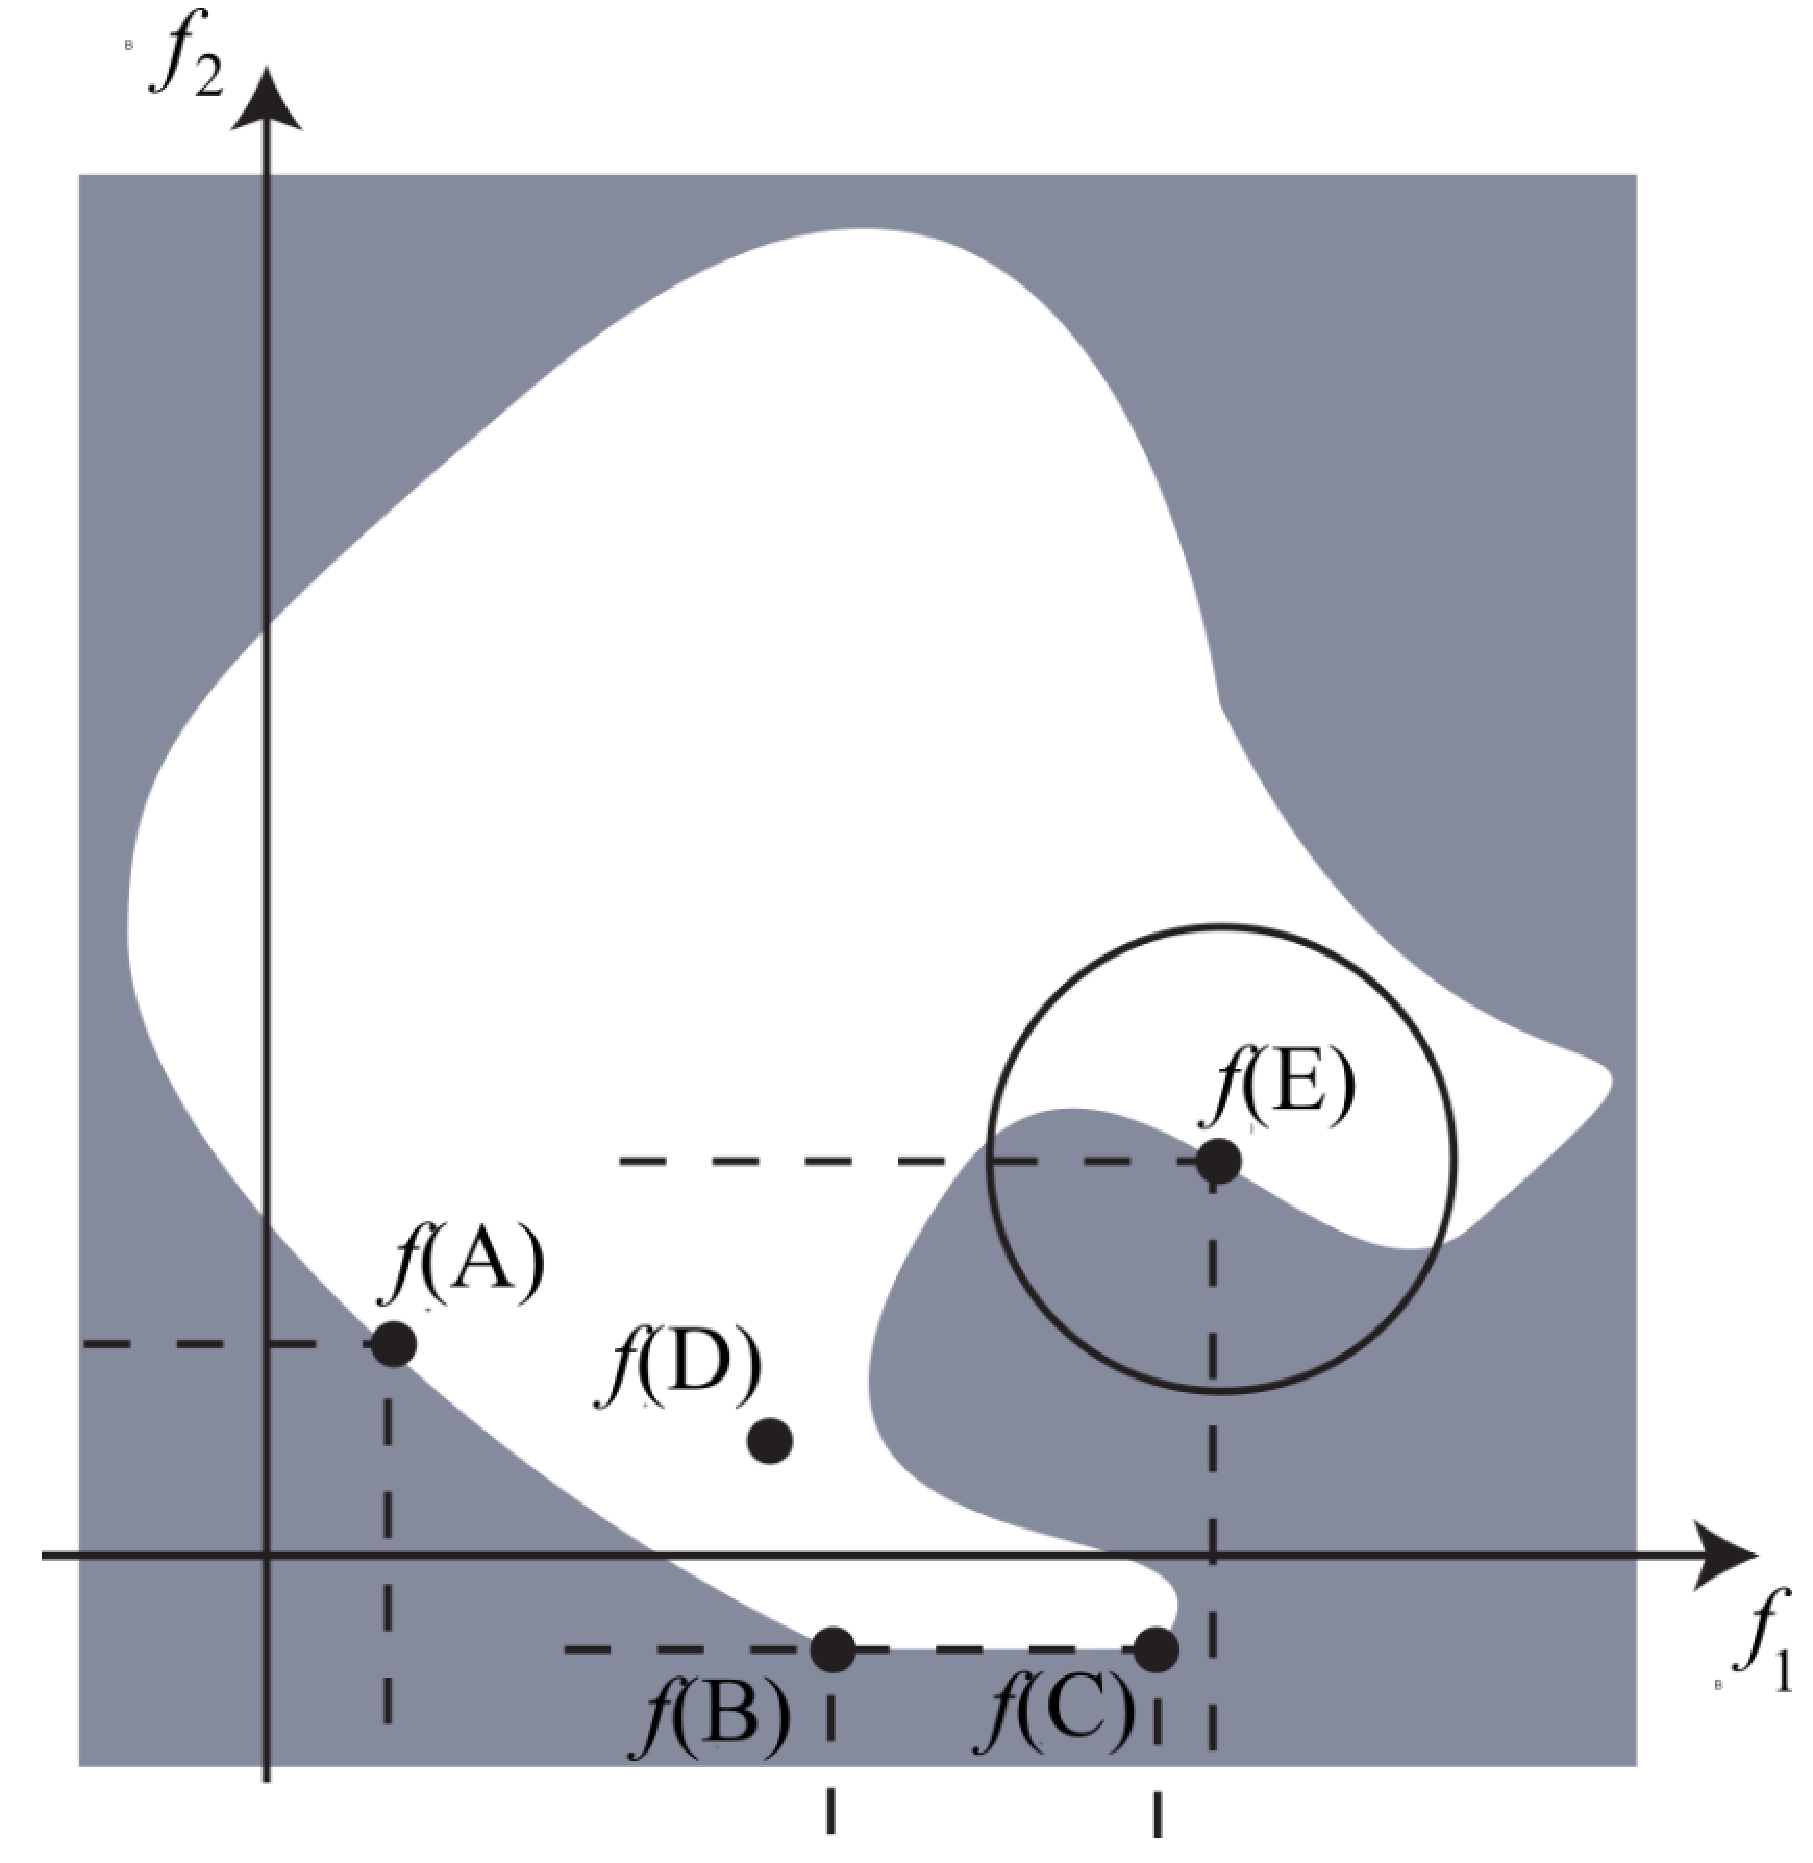
\includegraphics[width=0.5\columnwidth]{img/mcp/paretian/locpar}
\end{center}

We can see that
\begin{itemize}
	\item $D$ is dominated: there are impacts below and on the left of $f(D)$
	
	\item $A$ and $B$ are globally Paretian: their lower left quadrant is empty
	
	\item $E$ is locally Paretian: the quadrant is empty in a neighborhood
	
	\item $C$ is weakly Paretian: one indicator value is identical
\end{itemize}

If $X$ is discrete, all feasible solutions are isolated points, this means that, with a small enough $\epsilon$, every point can be locally Paretian with respect to $\U_{x, \epsilon}$. In the discrete case, once again, the overestimate given by the KKT conditions reduces to the whole set of feasible solutions.

\subsubsection{Sketch of the proof}

\paragraph{Definition} If a point $x$ is locally Paretian, all the arcs $\xi$ feasible in $x$ are nonimproving.

\paragraph{Nonimproving condition} We replace all indicators with their first-order approximation. The directions in which indicator $f_l$ is nonimproving satisfy condition $(\nabla f_l (x))^T p \geq 0$.\\

\begin{theo}
	If $\xi (\alpha)$ is a feasible arc in $x$ and $\nabla f_l (x)^T p < 0$ for all $l \in P$, then $x$ is not a locally Paretian point.
\end{theo}

It is a sufficient condition to prove that $\xi(\alpha)$ is an improving arc for $f(\cdot)$ in $x$, and therefore to filter $x$ out of the candidate set $X^{KKT}$.

Notice that improving all indicators is not necessary for strict dominance: weakly Paretian points are dominated, but some indicators can't improve. Therefore, weakly Paretian points satisfy the KKT conditions.

\paragraph{Feasibility condition} Feasibility is treated the same way as in Mathematical Programming: 
\begin{itemize}
	\item nonregular points are candidate
	
	\item a regular point $x$ is feasible if and only if
	$$ \nabla g_j(x)^T p \leq 0, \ \forall j \in J_a (x) $$
\end{itemize}

\paragraph{First geometric interpretation} Combining feasibility and nonimprovement implies that, if a point $\tilde x$is regular and locally Paretian and $p$ is a vector such that $(\nabla g_j)^Tp < 0$ for all constraints active in $\tilde x$ (vector tangent to a feasible arc), then there exists at least one indicator $f_l$ such that $(\nabla f_l)^T p \geq 0$ (an indicator that does not strictly improve along the arc).

Remembering the definition of feasible and improving cones (see \ref{subsec:firstgeometricinterpretation}), if a regular point is locally Paretian, then its feasible cone and improving cone do not intersect.
$$ x \in X^\ast \implies C_{feas} (x) \cap C_{impr} (x) = \emptyset $$

\paragraph{Farkas' lemma} The application of Farkas' lemma is somewhat more complicated than in Mathematical Programming, because there is no longer a single vector on one hand and a cone on the other. The workaround is to introduce an auxiliary vector and apply the lemma twice: to the auxiliary vector and the feasible cone and to the opposite of the auxiliary vector and the improving cone.

The existence of two cones which do not intersect is equivalent to the existence of hyperplane separating them that has two opposite orthogonal vectors: 
\begin{itemize}
	\item Vector $\gamma$ is on the opposite side of all $p \in C_{feas}$
	$$ p^T \gamma \leq 0, \ \forall p : p^T \nabla g_j (x) \leq 0, \ \forall j \in J_a (x) $$
	
	\item Vector $- \gamma$ is on the opposite side of all $p \in C_{impr}$
	$$ p^t (- \gamma) \leq 0, \ \forall p : \nabla f_l (x)^T (-p) < 0, \ \forall l \in P $$
\end{itemize}
Now we can apply Farkas' lemma to both expressions, obtaining that
\begin{itemize}
	\item Vector $\gamma$ falls in the cone of the gradients of the active constraints
	$$ \exists \mu_j \geq 0 : \gamma = \sum_{j \in J_a (x)} \mu_j \nabla g_j (x) $$
	
	\item Vector $- \gamma$ falls in the cone of the gradients of the objectives
	$$ \exists w_l \geq 0: - \gamma = \sum_{l \in P} w_l \nabla f_l (x) $$
\end{itemize}
Summing the two equations, one obtains the thesis:
$$ \exists \mu_j\geq 0, \ w_l \geq 0 : \sum_{l \in P} w_l \nabla f_l (x) + \sum_{j \in J_a (x)} \mu_j\nabla g_j (x) = 0$$
These are the KKT conditions for the Paretian case.

\paragraph{Standard form of the KKT-conditions} As in Mathematical Programming, the nonactive constraints can be reintroduces by imposing that their multipliers be zero, thanks to the complementarity conditions $\mu_j g_j (x) = 0$, and the equality constraints can be treated without explicitly replacing them with pairs of inequalities through the use of free multipliers.

Notice that, for any solution $(x, w, \mu)$, also $(x, \alpha w, \alpha \mu)$ is a solution, that provides the same candidate point $x$ (for any $\alpha > 0$). In other words, the multipliers have a degree of freedom that does not affect the solution. 

To remove this freedom we impose a normalization condition. Usually this is done by dividing all multipliers by $\sum_{l = 1}^p w_l$ so that
$$ \sum_{l = 1}^p w_l = 1$$

This requires to prove that $\sum_l w_l > 0$, but this is true because the gradients of the active constraints are linearly independent in all regular points and therefore $\sum_j \mu_j \nabla g_j \neq 0$.

\paragraph{Equation balance} The KKT condition system has $n+p+m$ variables: 
\begin{itemize}
	\item $n$ variables for vector $x$
	
	\item $p$ variables for vector $w$
	
	\item $m$ variables for vector $\mu$
\end{itemize}
and $n+1+m$ equalities
\begin{itemize}
	\item $n$ equations for the KKT conditions
	
	\item $1$ equation for the normalization condition
	
	\item $m$ equations for the complementarity conditions
\end{itemize}

In general, it will have $\infty^{p-1}$ solutions describing a hypersurface.

% End L10, notes p174

\section{The weighted-sum method}
\label{sec:weightedsum}

The weighted-sum method consists in building a linear combination of the indicators and minimizing it. The result is a sufficient condition for a point to be globally Paretian. \\

\begin{theo}
	Let $z(x) = \sum_{l = 1}^p w_l f_l (x)$ be a convex combination of the indicators, with coefficients $w_l > 0$ for $l \in \{1, \dots, p\}$ and $\sum_{l = 1}^p w_l = 1$. If $x^\circ$ is a globally optimal point for problem 
	$$ \min_{x \in X} z(x) \sum_{l = 1}^p w_l f_l (x) $$
	then $x^\circ$ is a globally Paretian point with respect to the impact $f(x)$.
\end{theo}
\begin{proof}
	The proof is by contradiction. If $x^\circ$ were not a Paretian point, by definition there should exist another point $x' \in X$ such that $x' \prec x^\circ$, that is $f_l (x') \leq f_l(x^\circ)$ for each $l \in \{1, \dots, p\}$, and an index $\bar l$ such that $f_{\bar l} (x') < f_{\bar l} (x^\circ)$. But this would imply
	$$ 
	\begin{cases}
		w_l f_l (x') & \leq w_l f_ (x^\circ), \ \forall l \in \{1, \dots, p\} \setminus \{\bar l\} \\
		w_{\bar l} f_{\bar l} (x') & < w_{\bar l} f_{\bar l} (x^\circ)
	\end{cases}
	$$
	Notice that the second property holds only if $w_{\bar l}$ is strictly positive. Summing the $p$ inequalities, one obtains
	$$ \sum_{l = 1}^p w_l f_l (x') < \sum_{l = 1}^p w_l f_l (x^\circ) \implies z(x') < z(x^\circ) $$
	and therefore $x^\circ$ cannot be a globally optimum point for $z(x)$. From the contradiction the thesis follows.\\
\end{proof}

The combination is convex, but the weights $w_l$ are strictly positive. If weights equal to zero were allowed, the proof would not hold, because weakly Paretian solutions satisfy the condition, even if dominated.

Let $W = \left\{w \in \R^p \mid w_l > 0, \ \forall l \in P, \ \sum_{l \in P} w_l = 1 \right\}$ be the weight space. \\

\begin{definition}
	Given a Paretian solution $x^\circ \in X^\circ$, we denote as \textbf{support} of $x^\circ$ the set $\supp(x^\circ) \subset W$ of weight vectors $w$ such that $x^\circ$ is a globally optimal point for the problem $\min_{x \in X} \sum_{l = 1}^p w_l f_l (x)$.
\end{definition}

Continuous problems usually have $\infty^{p-1}$ Paretian solutions and $\infty^{p-1}$ weight vectors: the support of a Paretian solution often includes a single vector. 

Finite or combinatorial problems have a finite number of solutions: the support of a Paretian solution often is a region in the weight space. 

In general, however, unsupported solutions exist. The weighted-sum method finds only supported solutions. \\

\begin{definition}
	We denote as \textbf{supported solution} a Paretian solution $x^\circ \in X^\circ$ whose support is nonempty: $\supp (x^\circ) \neq \emptyset$.
\end{definition}

The assumptions of the weighted-sum method are stricter than the KKT conditions (solution $x^\circ$ be a globally optimal point instead of candidate locally optimal ones, and strictly positive coefficients $w_l$ are imposed), making them sufficient to guarantee a point being Paretian, instead of only necessary. Consequently, this yields $X^{WS} \subseteq X^\circ$, subset instead of superset.

\paragraph{Combinatorial Example} Given a complete graph of three vertices and two cost function, find the minimum spanning tree
\begin{center}
	\begin{tabular}{c | c c c}
		$f(x)$ & $(1,2)$ & $(1,3)$ & $(2,3)$ \\
		\hline
		$f_1$ & 1 & 3 & 6 \\
		$f_2$ &13 & 10 & 8 
	\end{tabular}
\end{center}
The KKT-conditions are useless in this case, since it's a discrete problem, and therefore all solutions are locally Paretian. The inverse transformation method is usually impossible to apply in combinatorial problems, because of the exponential nature of the number of isolated points and impacts. 

There are three feasible solutions: 
\begin{center}
	\begin{tabular}{c | c c}
		$X$ & $f_1$ & $f_2$ \\
		\hline 
		$T_1 = \{(1,2), (1,3)\}$ & 4 & 23 \\
		$T_2 = \{(1,2), (2,3)\}$ & 7 & 21 \\
		$T_1 = \{(1,3), (2,3)\}$ & 9 & 18 \\
	\end{tabular}
\end{center}

Applying the definition, all solutions are Paretian: $X^\circ = \{T_1, T_2, T_3\}$. All solutions correspond to impacts with an empty lower left quadrant:
\begin{center}
	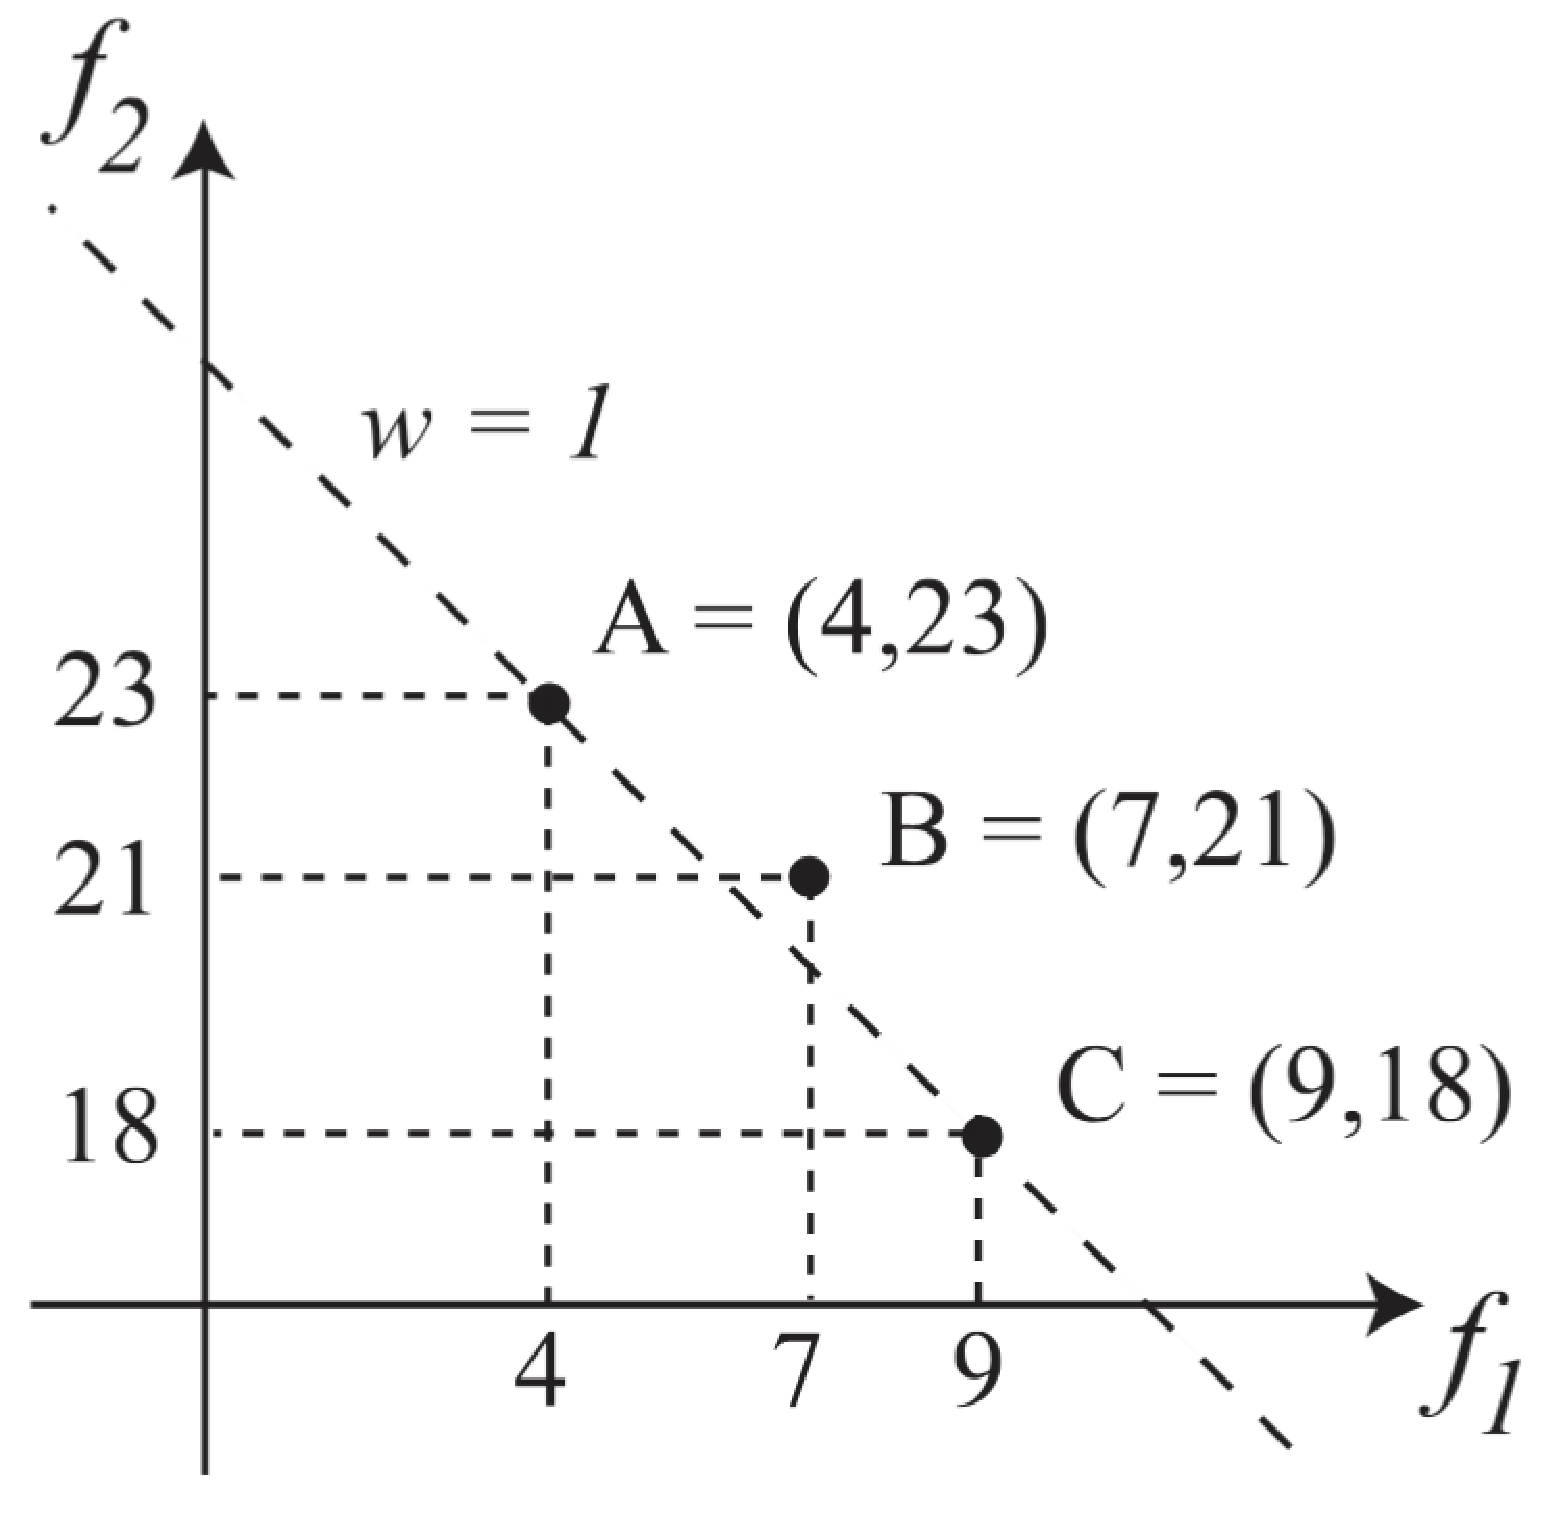
\includegraphics[width=0.4\columnwidth]{img/mcp/paretian/combex}
\end{center}

The weighted sum method solves the auxiliary parametric 
$$ \min z_w (x) = w f_1 (x) + (1 - w) f_2 (x) $$
combining the objectives $f_1$ and $f_2$ with the weights $w$ and $(1-w)$, where $w \in (0,1)$, and solving the minimum spanning tree problem for each value of $w$. The costs of the edges are:
\begin{itemize}
	\item $f(1,2) = w \cdot 1 + (1 - w) \cdot 13 = 13 - 12 w$
	
	\item $f(1,3) = w \cdot 3 + (1 - w) \cdot 10 = 10 - 7 w$
	
	\item $f(2,3) = w \cdot 6 + (1 - w) \cdot 8 = 8 - 2 w$
\end{itemize}

Making the problem
$$ \min z_w (x) = (13 - 12w) x_{12} + (1-7w)x_{13} + (8-2w)x_{23} $$
where $x$ is a spanning tree.

It's a minimum spanning tree with parametric costs on the edges $c_{ij} (w)$. The problem can be solved with Kruskal's algorithm: 
\begin{itemize}
	\item Sort the edges by increasing costs
	
	\item Include the edges that do not close loops
\end{itemize}

Let the weight vector $w$ vary in the weight space $W$, here $(0,1)$ and describe the costs $c_{ij} (w)$ of the three edges as a function of $w$.

\begin{center}
	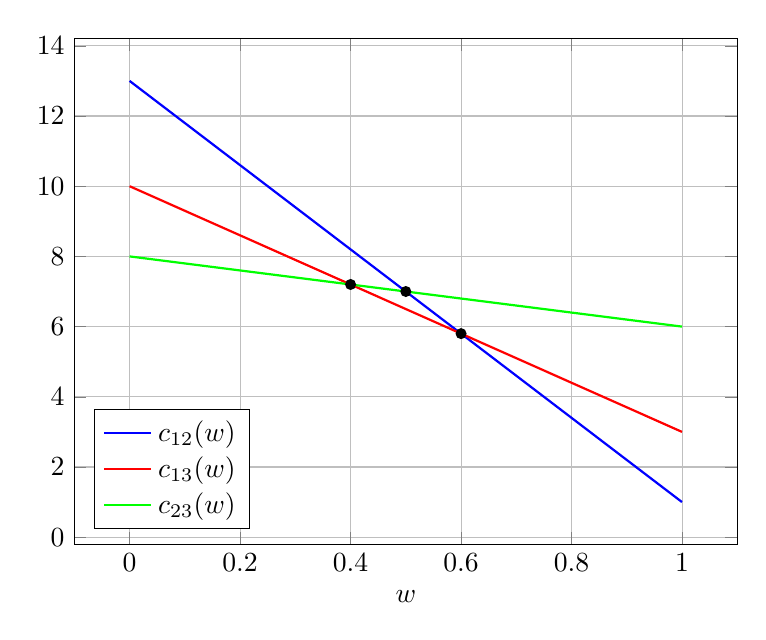
\begin{tikzpicture}
		\begin{axis}[
			xlabel={$w$},
			grid=major,
			legend pos=south west,
			domain=0:1,
			samples=100,
			width=10cm,
			height=8cm
			]
			%Functions
			\addplot[blue, thick, name path=c12] {13-12*x};
			\addlegendentry{$c_{12}(w)$}
			\addplot[red, thick, name path=c13] {10-7*x};
			\addlegendentry{$c_{13}(w)$}
			\addplot[green, thick, name path=c23] {8-2*x};
			\addlegendentry{$c_{23}(w)$}
			
			% Find intersections
			\path[name intersections={of=c12 and c13, name=int1}];
			\path[name intersections={of=c12 and c23, name=int2}];  
			\path[name intersections={of=c13 and c23, name=int3}];
			% Mark the intersection points
			\fill[black] (int1-1) circle (2pt);
			\fill[black] (int2-1) circle (2pt);
			\fill[black] (int3-1) circle (2pt);
		\end{axis}
	\end{tikzpicture}
\end{center}

Find the regions in $W$ where each arc is the cheapest, second, etc. (intersections of the lines shown above)
$$ c_{23} (w) = c_{13} (w) \Leftrightarrow w = \frac{2}{5}$$
$$ c_{13} (w) = c_{12} (w) \Leftrightarrow w = \frac{3}{5}$$
$$ c_{23} (w) = c_{12} (w) \Leftrightarrow w = \frac{1}{2}$$

Apply Kruskal's algorithm to each region: 
\begin{itemize}
	\item If $w \in (0, 2/5]$, select $(2,3)$ and $(1,3)$ $ \implies T_3 $
	
	\item If $w \in [2/5, 3/5]$, select $(1,3)$, then
	\begin{itemize}
		\item if $w \in [2/5, 1/2]$, select $(2,3)$ $ \implies T_3 $
		
		\item if $w \in [1/2, 3/5]$, select $(1,2)$ $ \implies T_1 $
	\end{itemize}
	
	\item If $w \in [3/5, 1)$, select $(1,2)$ and $(1,3)$ $ \implies T_1 $
\end{itemize}

Solution $T_2$ is not found: it is unsupported ($\supp(T_2) = \emptyset$). Indeed, $T_2$ is nonoptimal for any convex combination of the indicators, even if it can be a good compromise.

\subsection{Advantages and Disadvantages}
\label{subsec:wsprocons}

The weighted-sum method has some strong advantages: 
\begin{enumerate}
	\item It can be applied to any problem, even the ones for which KKT conditions are useless (e.g., discrete problems)
	
	\item It's very intuitive, as often the decision-makers find it natural to combine the indicators by summing them, after choosing units of measure for which their numerical values are not too different
	
	\item It only requires to build an auxiliary object for the problem, keeping every other feature, and in particular the feasible region; quite often, a valid algorithm for the optimization of the single indicators is also valid for the optimization of the auxiliary objective
\end{enumerate}

At the same time it has strong disadvantages:
\begin{enumerate}
	\item It requires to consider all possible values of the weight vector $w$, which form a continuous infinite set; this requires a parametric solution, that is in general nontrivial, and for large-size problems can become intractable
	
	\item It requires to find all globally optimal solutions for each value of $w$ (one is not enough, contrary to Mathematical Programming)
	
	\item It does not provide the whole Paretian region $X^\circ$, but only the supported solutions, which could be a very restrictive underestimate \\
\end{enumerate}

\begin{theo}
	In a combinatorial problem, the number of nonsupported solutions can grow exponentially with respect to the number $n$ of decision variables; correspondingly, the weighted-sum method can provide a fraction of the Paretian region gradually converging to zero.
\end{theo}

To avoid the need for a parametric algorithm, it's possible to sample the set of weights $W$, but this further reduces the subset found and it can be inefficient (finding the same solution for several different weight vectors).

\subsubsection{Relations between the weighted-sum method and MAUT}

There are strong similarities between the weighted-sum method to determine the Paretian region and the MAUT (additive utility function and the auxiliary problem look similar), but the context is completely different:
\begin{enumerate}
	\item The weighted-sum method does not require complete preferences, nor mutual preferential independence or the corresponding trade-off condition, but only that the attributes be costs or benefits; partial order instead of a weak order
	
	\item The weighted-sum method does not require to determine a specific weight vector $w$, but it scans all possible vectors with strictly positive components; in MAUT the weights $w_l$ have a fixed value in $W$
	
	\item The weighted-sum method does not provide an "optimal" solution but a subset of the Paretian region 
	
	\item The weighted-sum method directly combines the attributes, without filtering them through utility functions suitably built so as to reflect the relative utilities associated to different values of an indicator; consequently, it cannot access the nonsupported solutions; on the contrary, suitable utility functions (suitably shaped indifference curves) allow the overall utility function to admit such solutions as optimal; MAUT can reach unsupported solutions
\end{enumerate}

\section{The $\epsilon$-constraint method}
\label{sec:epsconstraint}

The $\epsilon$-constraint method consists in replacing all indicators but one with constraints that require the solution to respect a quality threshold, and in solving the resulting auxiliary problem. The result is a necessary condition for a point to be globally Paretian (sufficient and necessary to be weakly Paretian).

The following theorem proves that all Paretian solutions are optimal points for a problem of this family, provided that the thresholds are suitably determined. \\

\begin{theo}
	If $x^\circ$ is a globally Paretian point for $f$ in $X$, $\epsilon_l = f_l (x^\circ)$ and $\ell \in P$, then $x^\circ$ is globally optimal for
	$$ \min z_\epsilon = f_\ell (x), \quad \forall x \in X $$
	$$ f_l \leq \epsilon_l, \quad l \in P \setminus \{\ell\}$$
\end{theo}
\begin{proof}
	The proof is by contradiction: suppose that $x^\circ$ is not globally optimal:
	$$ \exists x' \in X : \begin{cases}
		f_\ell (x') < f_\ell (x^\circ) \\
		f_l (x') \leq \epsilon_l = f_l (x^\circ) \ l \in P \setminus \{\ell\}
	\end{cases} \implies x' \prec x^\circ $$
	which goes against the paretianity of $x^\circ$. \\
\end{proof}

The auxiliary problem is parametric, to be solved for all vectors $\epsilon \in \R^{p-1}$ ($\infty^{p-1}$ values). Consequently, the solutions provided form a hypersurface of $\infty^{p-1}$ points.

\subsubsection{$\epsilon$-constraint and lexicographic preference}

The lexicographic method also focuses on a single indicator. \textit{Is there a relation with the $\epsilon$-constraint method?}

Not really, since lexicographic preference: 
\begin{itemize}
	\item Assumes a total order on impacts, not a partial order
	
	\item Discriminates optimal impacts based on the secondary indicator
	
	\item Doe snot impose aspiration levels $\epsilon_l$ on the secondary indicators
\end{itemize}

\subsection{Advantages and disadvantages}

The $\epsilon$-constraint method has some strong advantages:
\begin{enumerate}
	\item It can be applied to any problem, even the ones for which KKT conditions are useless (e.g., discrete problems)
	
	\item It's very intuitive, as often decision-makers find it natural to focus on a single indicator and to translate their preference into minimum satisfaction thresholds
	
	\item It provides an overestimate of the Paretian region that is often quite tight and can be easily refined applying again the method with a different choice of the main indicator
\end{enumerate}

At the same time, however, it has strong disadvantages: 
\begin{enumerate}
	\item It requires to consider all possible values of thresholds $\epsilon$, which form a continuous infinite set; this requires a parametric solution, that is in general nontrivial, and for large size problems can become intractable
	
	\item It requires to find all globally optimal solutions for each value of $\epsilon$ (one is not enough, contrary to Mathematical Programming)
	
	\item In combinatorial problems, while changing the objective function usually does not affect the computational complexity of the problem (the polynomial ones remain polynomial), introducing additional constraints nearly always increases the complexity (for example, a polynomial problem turns into an NP-complete one)
\end{enumerate}

% End L11, p203 notes, skipping excercises
	% !TeX spellcheck = en_US
\chapter{Weak rationality methods}
\label{ch:wrm}

\section{Partially inconsistent decision-makers}
\label{sec:partiallyinconsistent}

The process of MAUT is tedious, complex and error prone. In practice, the problem is that decision-makers are usually unable to estimate correctly the rates of substitution as required by the theory, because they also consider indifferent pairs of impact between which there is a slight preference. The result is that the computation of the weights $w_l$ based on $p-1$ pairs of indifferent impacts is unreliable.

We assume:
\begin{itemize}
	\item A preference relation $\Pi$ that is a weak order with an additive utility
	
	\item A certain environment: $|\Omega| = 1 \implies f(x, \omega)$ reduces to $f(x)$
	
	\item A single decision maker: $|D| = 1 \implies \Pi_d$ reduces to $\Pi$
\end{itemize}

However: 
\begin{itemize}
	\item The pairwise comparison matrix $\tilde \Lambda$ is incorrect
	
	\item The normalized utilities $\mu u(f_l)$ are incorrect
\end{itemize}
Therefore, $u(f) = \sum_{l \in P} w_l \tilde u_l (f_l)$ makes no sense-

The normalized utilities $\tilde u _l (x)$ and the pairwise comparison coefficients $\tilde \lambda_{lm}$ are only approximated ($\tilde \Lambda$ is typically positive and reciprocal, but inconsistent, giving nonunivocal weight vectors), and the approximations of $w_l$ and $\tilde u_l (x)$ combine in cascade.
$$ \tilde u(x) = \sum_{l \in P} \left(w_l \pm \delta w_l \right) \left(\tilde u_l (x) \pm \delta \tilde u_l (x)\right) $$

\section{Reconstructing consistent matrices}
\label{sec:reconstrconsistent}

A possible approach is to force consistency modifying $\tilde \Lambda$ as little as possible. This requires a definition of distance between matrices.

Given a metric $d: \R^{p^2} \times \R^{p^2} \rightarrow \R$, we can solve the problem
$$ \min d\left(W, \tilde \Lambda \right) $$
$$ W_{lm} = \frac{w_l}{w_m} $$
$$ w_l > 0, \quad l \in P, \quad \sum_{l \in P} w_l = 1$$
where the unknown variables are the weights $w_l$, $W$ denotes the matrix composed by the ratios $w_l/w_m$, $\tilde \Lambda$ the matrix denoted by the ratios estimated by the decision-maker and $d$ is a distance.

This is done in order to determine an unknown matrix $W$ that is 
\begin{itemize}
	\item positive, reciprocal and consistent
	
	\item as close as possible to the known matrix $\tilde \Lambda$
\end{itemize}

There are infinite possible definitions of distances, the choice is arbitrary, and the optimal matrix $W^\circ$ depends on the distance chosen. Examples: 
\begin{itemize}
	\item Manhattan distance $L_1$:
	$$ d_1 \left(W, \tilde \Lambda\right) = \sum_{l,m \in P} \left|\frac{w_l}{w_m} - \tilde \lambda_{lm} \right|$$
	
	\item Euclidean distance $L_2$:
	$$ d_2 \left(W, \tilde \Lambda\right) = \sqrt{\sum_{l,m \in P} \left(\frac{w_l}{w_m} - \tilde \lambda_{lm} \right)^2} $$
	
	\item $L_{\infty}$ distance:
	$$ d_{\infty} \left(W, \tilde \Lambda\right) = \max_{l,m \in P} \left|\frac{w_l}{w_m} - \tilde \lambda_{lm} \right| $$
\end{itemize}

\subsubsection{The eigenvalue method}

Another way to achieve consistency exploits the following properties: given a square matrix $\tilde \Lambda$ of order $p \times p$
\begin{itemize}
	\item eigenvalues are the $p$ solutions of equation $|\lambda l - \tilde \Lambda|$
	
	\item eigenvectors associated to $\lambda$ are the $\infty$ nonzero solutions of $\lambda x = \tilde \Lambda x$
\end{itemize}

If $\tilde \Lambda$ is positive, reciprocal and consistent
\begin{itemize}
	\item The dominant (maximum absolute value) eigenvalue is $\lambda_{\max} = p$
	
	\item The other $p-1$ eigenvalues are equal to zero ($\tilde \Lambda$ has rank 1)
	
	\item The eigenvectors associated to $\lambda_{\max}$ are proportional to the weight vector, and $w$ is the normalization of any dominant eigenvector $x_{\max}$
\end{itemize}

Consequently, the \textbf{eigenvalue method} proposes to
\begin{enumerate}
	\item Compute the eigenvalues and identify the dominant one $\lambda_{\max}$
	
	\item Compute the associated dominant eigenvector $x_{\max}$
	
	\item Normalize it to obtain the weight vector $w = \frac{x_{{\max}}}{\|x_{\max}\|}$
	
	\item Build the correct matrix as $W = \left\{\frac{w_l}{w_m}\right\}$
\end{enumerate}

But the resulting matrix $W$ can be far from $\tilde \Lambda$, other consistent matrices could be closer. Can a forcedly consistent matrix be safely used? This is subject of debate.

An alternative approach is to 
\begin{itemize}
	\item Consciously accept imprecise values for $w_l$ and $\tilde u_l (x)$ 
	
	\item Compute them based on the stronger aspects of human psychology
	
	\item Aim at a qualitative ranking, instead of a quantitative one
\end{itemize}

\section{Analytic Hierarchy Process AHP}
\label{sec:ahp}

The Analytic Hierarchy Process (AHP) by Saaty (1980): 
\begin{itemize}
	\item Replaces absolute measures with relative ones
	
	\item Replaces quantitative ratios with qualitative scales 
	
	\item Builds a hierarchy of indicators in order to compare only conceptually similar quantities
\end{itemize}

\subsection{Computation of the utilities with pairwise comparisons}

Given an indicator $f_l$, the classical method tries to reconstruct the whole absolute profile of a utility function $\tilde u_l (f_l)$, but psychology says that it's difficult for a human decision-maker to associate quantitative utility values to the values of the indicator.

The AHP focuses on pairs of solutions and on the strength of the relative preference between the values of an indicator in the two solutions of the pair. A matrix $\Lambda_l = \left\{\lambda_{xy}^{(l)}\right\}$ is built, whose element $\lambda_{xy}^{(l)}$ is associated to a pair of alternatives $(x,y) \in X \times X$ and evaluates how much $f_l (x)$ is preferable to $f_l (y)$.

This process evaluates the strength ratio between given pairs of alternatives, i a similar fashion to a utility ratio $\tilde u_l (f_l (x)) / \tilde u_l (f_l (x))$.

Since it requires the explicit enumeration of all solution pairs, the AHP can be applied \textbf{only to finite problems} and with a small number of solutions, or to problems whose solution set has been preliminarily pruned reducing it to a small finite set.

\subsection{Qualitative scales}

The second idea of the AHP is to measure the preference between values not with a quantitative scale but with a qualitative one, denoted as \textit{Saaty's scale}:
\begin{itemize}
	\item $\lambda_{xy}^{(l)} = 1$ for $f_l (x)$ \textit{equally good} as $f_l (y)$
	
	\item $\lambda_{xy}^{(l)} = 3$ for $f_l (x)$ \textit{moderately better} than $f_l (y)$
	
	\item $\lambda_{xy}^{(l)} = 5$ for $f_l (x)$ \textit{strongly better} than $f_l (y)$
	
	\item $\lambda_{xy}^{(l)} = 7$ for $f_l (x)$ \textit{very strongly better} than $f_l (y)$
	
	\item $\lambda_{xy}^{(l)} = 9$ for $f_l (x)$ \textit{absolutely better} than $f_l (y)$
\end{itemize}

The weights $2$, $4$, $6$ and $8$ are used for intermediate evaluations. The values are arbitrary, but they derive from the psychological fact that human decision-makers can't discriminate between more that $5$ levels in a reliable way.

Moreover, the use of a qualitative scale allows to compare heterogeneous quantities not expressed in a quantitative way, translating verbal judgments into numerical values. The idea is to give for granted that the values used are only a rough approximation, automatically raising an alert against trusting them too much. 

Building a whole pairwise comparison matrix also allows to evaluate its inconsistency and to tune it \textit{a posteriori} in order to make it consistent, instead of forcing a fictitious consistency since the beginning, which could introduce errors. \\

\begin{definition}
	We denote as \textbf{evaluation matrix} a matrix $U = \{u_{xl}\}$ containing the evaluation $u_{xl}$ of each alternative $x \in X$ with respect to each indicator $l \in P$, obtained starting from the pairwise comparison matrix $\Lambda_l$.
\end{definition}

The same qualitative process is followed for the weight ratios $\tilde \lambda_{lm} = \frac{w_l}{w_m}$ for each $l,m \in P$:
\begin{itemize}
	\item Choose representative qualitative values $\lambda_{lm}$
	
	\item Impose consistency 
	
	\item Derive pseudoweights $w_l$ from the consistent matrix
\end{itemize}

\subsection{Hierarchical structuring of the attributes}

Humans are bad at comparing nonhomogeneous things, so the idea is to build an indicator tree and compare only siblings indicators:
\begin{itemize}
	\item The level of the leaves includes the elementary attributes
	
	\item At the upper levels summarizing attributes appear, progressively more general
	
	\item The root corresponds to a sort of general objective
\end{itemize}

The idea of this process has already been discussed in Chapter \ref{ch:cases}.

Instead of comparing $l$ and $m$ for each $l,m \in P$
\begin{itemize}
	\item Estimate weight ratio $\lambda_{lm}$ only when $l$ and $m$ have the same father
	
	\item Perform comparisons at all levels of the indicator tree, not only between indicators, but also between indicator groups
\end{itemize}
Replace a single big pairwise comparison matrix with many small ones.

The advantages of structuring the attributes into a hierarchy are:
\begin{itemize}
	\item Only homogeneous attributes are compared with each other
	
	\item Each subset of pairwise comparisons can be assigned to an expert decision-maker, specialized in a specific field, so as to obtain more meaningful indications
	
	\item The total number of pairwise comparisons strongly decreases
\end{itemize}

The fundamental disadvantage is that the pairwise comparisons at the level of the leaves consider concrete and well-defined attributes, whereas those at the upper levels consider abstract and general objectives, for which a quantitative measure does not even make sense.

\subsection{Hierarchical recomposition}

The weights are normalized within each group of children nodes, but are not comparable with those of other group. The tree structure, however, allows to progressively build the attribute weight vector scanning the tree level-by-level from the leaves up to the root.

At each level, one builds a pairwise comparison matrix between the children of the same node, and derives from it a vector of weights with the methods described above. The weights in each vector have sum equal to one, and describe the relative weight between each other. In order to compare such weights with those of the other nodes of the whole tree, it is enough to renormalize them so that their sum coincides with the weight of the father node, that is simply to multiply them by the weight of the father node.

Given the pseudoutilities $\tilde u_{lx}$ and the pseudoweights $w_l$: 
\begin{itemize}
	\item Combine them with convex combinations
	
	\item Combine the pseudoweights with products from root to leaf, this corresponds to normalizing each set of sibling nodes
	$$ u(x) = \sum_{l \in P} \prod_{\ell \in \gamma_l} w_\ell \tilde u_{lx} $$
\end{itemize}

\subsection{Rank reversal}

The main defect of the AHP is the phenomenon of \textbf{rank reversal}: the order of the alternatives substantially depends on what alternatives are present. This happens because evaluations are pairwise comparisons and not absolute utility values, and therefore depend on the values actually compared.

In the AHP adding or removing alternatives can change the ranking, and alternatives can be generated in different phases, modifying the feasible region $X$.

A result depending on $X$ is undesirable, because. 
\begin{itemize}
	\item $X$ is not always given a priori
	
	\item Modifying $X$ allows to manipulate the result
\end{itemize}

Unfortunately, all decision processes based on pairwise comparisons between alternatives suffer from rank reversal (e.g., sport tournaments).

\subsubsection{Absolute scales, or \textit{a priori} estimate method}

In order to avoid rank reversal, Saaty proposed a system using absolute scales and a priori estimates: 
\begin{itemize}
	\item Fix a (finite) set of absolute levels for each indicator
	
	\item Make pairwise comparisons on levels, instead of alternatives 
	
	\item Evaluate each alternative assigning it to a level for each indicator
\end{itemize}

In this way, the pseudoutilities refer to absolute levels, fixed once for all, and not depending on the alternatives. Basically, define a number of levels and assign a value among these levels to each indicator.

The use of absolute classes also allows:
\begin{itemize}
	\item Open decision processes, in which alternatives arrive gradually
	
	\item Very long decision processes, in which alternatives arriving at far away times cannot be compared significantly
	
	\item To end the process as soon an alternative reaches a satisfactory threshold 
\end{itemize}

However, the trick also introduces further approximations:
\begin{itemize}
	\item Rather different values can be flattened putting them into the same class 
	
	\item Very similar values can be strongly differentiated putting them into separate classes
\end{itemize}

% End L13, p220 notes
	
	\part{Models with multiple scenarios}
	
	% !TeX spellcheck = en_US
\chapter{Models of Uncertainty}
\label{ch:uncertainty}

The \textit{Programming in conditions of uncertainty} deals with decision problems in which the choice is among alternatives whose impact depends not only on the choice of the decision-maker, but also on external factors that cannot be exactly predicted.

These problems are characterized by having:
\begin{itemize}
	\item A preference relation $\Pi$ that is a weak order with a known consistent value function $u(f)$ (replaced by a cost $f$, a single objective)
	
	\item A single decision maker: $|D| = 1 \implies \Pi_d$ reduces to $\Pi$
	
	\item A uncertain environment: $|\Omega| > 1$, the impact of the decision depends also on variables which are not under the control of the decision-maker and about whose value only partial information is available
\end{itemize}

Such problem can be formulated as
$$ \min_{x \in X} f(x, \omega) $$
$$ \omega \in \Omega $$

Where:
\begin{itemize}
	\item $X$ is the set of the alternatives or solutions $x$ 
	
	\item $\Omega$ is the set of the scenarios $\omega$ (in statistics, \textit{sample space})
	
	\item $f(x, \omega)$ is the impact of solution $x$ and scenario $\omega$, $\in \R$
	
	\item Lower impacts are preferable to high ones (or vice versa)
\end{itemize}

The decision maker can choose the alternative $x$, but not the scenario $\omega$, and the choice of $x$ precedes the unraveling of $\gamma$. If $x$ were chosen after $\omega$, the problem would reduce to a Mathematical Programming problem parametrized in $\omega$.

The problems in conditions of uncertainty include two main classes, though other ones have been proposed: 
\begin{itemize}
	\item Decisions in condition of \textit{ignorance}: the only information on scenario $\omega$ is that it falls within $\Omega$
	
	\item Decisions in conditions of \textit{risk}: the probability $\pi_\omega$ of each scenario $\omega \in \Omega$ is known (if $\Omega$ is a discrete set) ot the probability density $\pi (\omega)$ is known (if $\Omega$ is a continuous set)
\end{itemize}

In all these classes, it's possible to define relations of dominance that allow to reduce the set of interesting solutions. In general, these relations will not lead to a single choice, as they typically are partial orders (reflexive, transitive but incomplete).

\section{Dominance relations}
\label{sec:domrel}

\begin{definition}
	We say that alternative $x$ \textbf{strongly dominates} alternative $x'$ when its impact is at least as good in all scenarios $\omega \in \Omega$
	$$ x \wpref{} x' \Leftrightarrow f (x, \omega) \leq f(x', \omega), \quad \forall \omega \in \Omega $$
\end{definition}

Similarly to the concept of Paretian preference, the alternative which are strictly dominated can be rejected a priori. \\

\begin{definition}
	In the finite case, the impact $f (x, \omega)$ can be represented with an \textbf{evaluation matrix} $U$, having the alternatives $x$ on the rows and all the scenarios on the columns.
\end{definition}

In order to find the nondominated alternatives, one must perform pairwise comparisons on the rows of the matrix, exactly as in the Paretian case. \\

\begin{definition}
	We say that alternative $x$ \textbf{probabilistically dominates} alternative $x'$ when for any threshold $\bar f$ the probability that $x$ have impacts not worse than the threshold is not inferior to that of $x'$.
	$$ x \wpref{} x' \Leftrightarrow P \left[f(x, \omega) \leq \bar f\right] \geq P \left[f (x', \omega) \leq \bar f\right], \quad \forall \bar f \in \R $$
\end{definition}

\section{Models of uncertainty}
\label{sec:modelsuncert}

There are two main ways to describe uncertain situations, that reflect into two main forms of the scenario set $\Omega$: 
\begin{itemize}
	\item \textit{Scenario description:} $\Omega$ is a finite set, in which the single scenarios are explicitly listed
	$$ \Omega = \left\{\omega^{(1)}, \dots, \omega^{(|\Omega|)}\right\} $$
	
	\item \textit{Interval description:} $\Omega$ is the Cartesian product of a finite number of real intervals $s$ on the exogenous variables
	$$ \Omega = \left[\omega_1^{\min}, \omega_1^{\max}\right] \times \dots \times \left[\omega_s^{\min}, \omega_s^{\max}\right]$$
\end{itemize}

These are not the only possible cases, $\Omega$ could assume more sophisticated forms. However they are two frequent special cases.

\textit{How to choose?} The appropriate description depends on: 
\begin{itemize}
	\item The precision of the representation
	
	\item The simplicity of the solution process
\end{itemize}

On one hand, the scenario description has a finite number of cases: 
\begin{itemize}
	\item Are they all and only the possible cases? 
	
	\item Are they few or combinatorially many? 
\end{itemize}

On the other hand, the interval description: 
\begin{itemize}
	\item Implies that the exogenous variables are independent (precision)
	
	\item The scenarios are infinitely many, but the worst scenario might be the same for all solutions or easy to find
\end{itemize}

% End L15? This was easy, p247 notes
	% !TeX spellcheck = en_US
\chapter{Decisions in conditions of ignorance}
\label{ch:ignorance}

Full ignorance is the most problematic situation for a decision-maker, since the information on the exogenous part of the problem reduces to knowing that the scenario falls within a given set.

We assume:
\begin{itemize}
	\item A preference relation $\Pi$ that is a weak order with a known consistent value function $u(f)$ (replaced by a cost $f$)
	
	\item A uncertain environment: $|\Omega| > 1$ and we have no other information
	
	\item A single decision-maker: $|D = 1| \implies \Pi_d$ reduces to $\Pi$
\end{itemize}

The idea is to aggregate all scenarios of $\Omega$ and reduce $f(x, \omega)$ to $\phi_\Omega (x)$. Various ways have been proposed, no approach can satisfy all desirable properties. \\

\begin{definition}
	We denote as \textbf{choice criterium} every definition of $\phi_\Omega (x)$ aimed to replace the impact $f(x, \omega)$.
\end{definition}

Each of the criteria we'll propose has some advantages, but none satisfies all the properties desirable for a rationally founded decision. 

We'll apply each criterium to an example with four alternatives ($X = \{x^{(1)}, x^{(2)}, x^{(3)}, x^{(4)}\}$) and four scenarios ($\Omega = \{\omega^{(1)}, \omega^{(2)}, \omega^{(3)}, \omega^{(4)} \}$), whose evaluation matrix is reported below (values are costs).

\begin{table}[h!]
	\centering
	\label{tab:fxomega}
	$$
	\begin{array}{c|cccc}
		f(x,\omega) & \omega^{(1)} & \omega^{(2)} & \omega^{(3)} & \omega^{(4)} \\
		\hline
		x^{(1)} & 2 & 2 & 4 & 3 \\
		x^{(2)} & 3 & 3 & 3 & 3 \\
		x^{(3)} & 4 & 0 & 4 & 6 \\
		x^{(4)} & 3 & 1 & 4 & 4 \\
	\end{array}
	$$
\end{table}


\section{Worst-case criterium}
\label{sec:wcc}

This criterium, also known as \textit{pessimism criterium} or \textit{Wald criterium} (from its inventor, \href{https://en.wikipedia.org/wiki/Abraham_Wald}{\texttt{Abraham Wald}}), consists in being pessimist and assuming that for each chosen solution $x$ the future prepare the scenario implying the largest cost
$$ w^\dag (x) = \arg \max_{\omega \in \Omega} f(x, \omega)$ $

This allows to compute the impact as a function only of the decision variable $x$, reducing the problem to the minimization of $\phi_{worst}(x) = f\left(x, \omega^\dag (x) \right)$
$$ \min_{x \in X} \phi_{worst} (x) = \min_{x \in X} \max_{\omega \in \Omega} f(x, \omega) $$

The table reports, for each alternative, the value of the criterium and the scenario that produces it.
$$
\begin{array}{c|cccc | c c}
	f(x,\omega) & \omega^{(1)} & \omega^{(2)} & \omega^{(3)} & \omega^{(4)}  & \phi_{worst} (x) & \omega^\dag (x) \\
	\hline
	x^{(1)} & 2 & 2 & 4 & 3 & 4 & \omega^{(3)} \\
	x^{(2)} & 3 & 3 & 3 & 3 & 3  & \omega^{(1)}, \omega^{(2)}, \omega^{(3)}, \omega^{(4)} \\
	x^{(3)} & 4 & 0 & 4 & 6 & 6 & \omega^{(4)} \\
	x^{(4)} & 3 & 1 & 4 & 4 & 4 & \omega^{(3)}, \omega^{(4)} \\
\end{array}
$$

Now it's enough to select the best alternative, i.e., the cheapest one. The worst-case criterium suggests to order the alternatives as follows
$$ x^{(2)} \prec x^{(1)} \sim x^{(4)} \prec x^{(3)} $$

It's a conservative approach: avoid losses, even giving up opportunities.

\section{Best-case criterium}
\label{sec:bcc}

The best-case criterium, also known as \textit{optimism criterium}, is complementary to that of the worst-case: for each solution $x$, assume that the scenario is the best possible
$$ \omega^\ast (x) = \arg \min_{\omega \in \Omega} f (x, \omega) $$

Similarly to before, this allows to compute the impact as a function only of the decision variable $x$, reducing the problem to a minimization of function $\phi_{best} (x) = f (x, \omega^\ast (x))$
$$ \min_{x \in X} \phi_{best} (x) = \min_{x \in X} \min_{\omega \in \Omega} f(x, \omega) $$

The table reports, for each alternative, the value of the criterium and the scenario that produces it.
$$
\begin{array}{c|cccc | c c}
	f(x,\omega) & \omega^{(1)} & \omega^{(2)} & \omega^{(3)} & \omega^{(4)}  & \phi_{best} (x) & \omega^\ast (x) \\
	\hline
	x^{(1)} & 2 & 2 & 4 & 3 & 2 & \omega^{(1)} \\
	x^{(2)} & 3 & 3 & 3 & 3 & 3  & \omega^{(1)}, \omega^{(2)}, \omega^{(3)}, \omega^{(4)} \\
	x^{(3)} & 4 & 0 & 4 & 6 & 0 & \omega^{(2)} \\
	x^{(4)} & 3 & 1 & 4 & 4 & 1 & \omega^{(2)} \\
\end{array}
$$

This suggests the ordering
$$ x^{(3)} \prec x^{(4)} \prec x^{(1)} \prec x^{(2)} $$

It's an opportunistic approach: believe in opportunities, ignoring dangers.

\section{Hurwicz criterium}
\label{sec:hurwicz}

The first two criteria are too biased towards extreme conditions. To have a stronger balance, \href{https://en.wikipedia.org/wiki/Leonid_Hurwicz}{\texttt{Leonid Hurwicz}} proposed a choice criterium making a convex combination of the two:
\begin{align*}
	\min_{x \in X} \phi_{Hurwicz} (x) & = \min_{x \in X} \left[\rho \phi_{worst}(x) + (1- \rho) \phi_{best} (x) \right] \\
	& = \min_{x \in X} \left[\rho \max_{\omega \in \Omega} f (x, \omega) + (1-\rho) \min_{\omega \in \Omega} f(x, \omega)\right]
\end{align*}
Where $\rho \in [0,1]$ is the \textit{pessimism coefficient}, as it weighs the worst impact, allowing to tune the weights of the two scenarios.

The table reports, for each alternative, the value of the criterium.
$$
\begin{array}{c|cccc | c}
	f(x,\omega) & \omega^{(1)} & \omega^{(2)} & \omega^{(3)} & \omega^{(4)}  & \phi_{Hurwicz} (x) (\rho = 0.6) \\
	\hline
	x^{(1)} & 2 & 2 & 4 & 3 & 0.6 \cdot 4 + 0.4 \cdot 2 = 3.2 \\
	x^{(2)} & 3 & 3 & 3 & 3 & 0.6 \cdot 3 + 0.4 \cdot 3 = 3 \\
	x^{(3)} & 4 & 0 & 4 & 6 & 0.6 \cdot 6 + 0.4 \cdot 0 = 3.6 \\
	x^{(4)} & 3 & 1 & 4 & 4 & 0.6 \cdot 4 + 0.4 \cdot 1 = 2.8 \\
\end{array}
$$

This suggests the ordering
$$ x^{(4)} \prec x^{(2)} \prec x^{(1)} \prec x^{(3)} $$

\subsection{Tuning the pessimism coefficient}

A possible approach to tune $\rho$ is to find (possibly, to invent) a pair of reciprocally indifferent alternatives, to impose the equality of the corresponding values of criterium $\phi_{Hurwicz} (x)$ and solve the resulting equation in $\rho$.

The simplest wa to do that is to choose an alternative $x$, then ask the decision-maker to indicate its \textit{certainty equivalent}, that is an alternative $y$, that in general is not a true alternative of the problem, with a uniform impact in all scenarios and that is overall indifferent to $x$.

Let us choose alternative $x^{(3)}$:  if the decision-maker states that an alternative $y$ with a uniform cost of 4 would be indifferent to $x^{(3)}$, we can conclude that $\phi_{Hurwicz}(x^{(3)}) = \phi_{Hurwicz} (y)$, that is
$$ \rho \phi_{worst} f (x^{(3)}) + (1 - \rho) \phi_{best} f(x^{3}) = \rho \phi_{worst} f(y) + (1-\rho) \phi_{best} (y) $$
$$ \implies 6 \rho + 0(1-\rho) = 4 \rho + 4(1-\rho) \implies \rho = \frac{2}{3} $$

It is not at all obvious that the decision-maker is able to indicate a certainty equivalent.

\subsection{Sensitivity analysis}

If the ranking is unclear and the value of $\rho$ imprecise, find the support of each solution $x$, i.e. the range of $\rho$ in where $x$ is optimal for $\phi_{Hurwicz} (x)$
$$ \supp (x) = \left\{\rho \in [0,1] \mid x \in \arg \min_{x \in X} \phi_{Hurwicz} (x) \right\}$$

The choice criterium $\phi_{Hurwicz} (x)$ becomes a linear function in $\rho$
\begin{itemize}
	\item $\phi_{Hurwicz} \left(x^{(1)}\right) = 4 \rho + 2(1 - \rho) = 2 \rho + 2$

	\item $\phi_{Hurwicz} \left(x^{(2)}\right) = 3 \rho + 3(1 - \rho) = 3$
	
	\item $\phi_{Hurwicz} \left(x^{(3)}\right) = 6\rho + 0(1 - \rho) = 6 \rho$ 
	
	\item $\phi_{Hurwicz} \left(x^{(4)}\right) = 4 \rho + 1 (1 - \rho) = 3 \rho + 1$
\end{itemize}

\begin{center}
	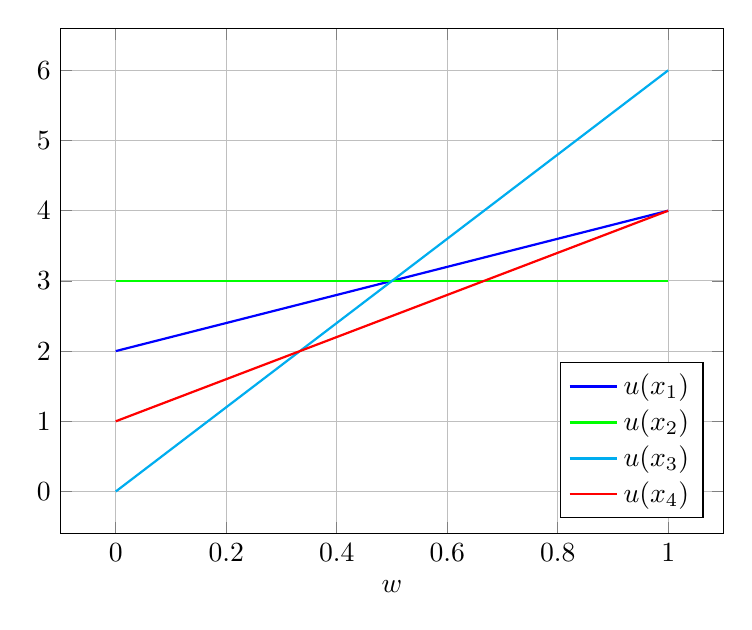
\begin{tikzpicture}
		\begin{axis}[
			xlabel={$w$},
			grid=major,
			legend pos=south east,
			domain=0:1,
			samples=100,
			width=10cm,
			height=8cm
			]
			%Functions
			\addplot[blue, thick, name path=1] {2*x+2};
			\addlegendentry{$u(x_1)$}
			\addplot[green, thick, name path=2] {3};
			\addlegendentry{$u(x_2)$}
			\addplot[cyan, thick, name path=3] {6*x};
			\addlegendentry{$u(x_3)$}
			\addplot[red, thick, name path=4] {3*x+1};
			\addlegendentry{$u(x_4)$}
		\end{axis}
	\end{tikzpicture}
\end{center}

The lower envelope of their profiles identifies the support. Basically, the part oof the domain for which that function does not have another function below it.

Notice that: 
\begin{itemize}
	\item The strictly dominated solutions are never optimal 
	
	\item Also some nondominated solutions have empty support (unsupported)
\end{itemize}

This is similar to the weighted sum method for Paretianity, but stronger: even solutions that are the best in a scenario can have empty support ($a_1$ is the best in $\omega_1$, but still unsupported).

The solution is
\begin{itemize}
	\item $x_3$ for $\rho \in \left[0, \frac{1}{3}\right]$
	
	\item $x_4$ for $\rho \in \left[\frac{1}{3}, \frac{2}{3}\right]$
	
	\item $x_2$ for $\rho \in \left[\frac{2}{3}, 1 \right]$
\end{itemize}

Notice that the result of all criteria considered depends on $\Omega$.

\section{Equiprobability criterium}
\label{sec:equiprob}

The equiprobability criterium, also known as \textit{Laplace criterium}, modifies Hurwicz criterium considering all scenarios, instead of only the extreme ones, applying the same weight on all of them:
$$ \min_{x \in X} \phi_{Laplace} (x) = \min_{x \in X} \frac{\sum_{\omega \in \Omega} f(x, \omega)}{|\Omega|} $$
when $f$ is a cost. This leads to a simple arithmetic mean of the impacts on the scenarios.

The table reports, for each alternative, the value of the criterium.
$$
\begin{array}{c|cccc | c}
	f(x,\omega) & \omega^{(1)} & \omega^{(2)} & \omega^{(3)} & \omega^{(4)}  & \phi_{Laplace} (x)\\
	\hline
	x^{(1)} & 2 & 2 & 4 & 3 & (2+2+4+3)/4 = 2.75 \\
	x^{(2)} & 3 & 3 & 3 & 3 & (3+3+3+3)/4 = 3.00 \\
	x^{(3)} & 4 & 0 & 4 & 6 & (4+0+4+6)/4 = 3.50 \\
	x^{(4)} & 3 & 1 & 4 & 4 & (3+1+4+4)/4 = 3.00 \\
\end{array}
$$

This suggests the ordering
$$ x^{(1)} \prec x^{(2)} \sim x^{(4)} \prec x^{(3)} $$

This is obviously possible only for finite scenario sets (actually, a generalization is possible). It's a balanced approach that keeps all scenarios into account.

\section{Regret criterium}
\label{sec:regret}

This criterium, also known as \textit{Savage criterium}, consists in evaluating the regret that the decision-maker would feel if the decision taken were wrong. The concept behind is that a solution should be compared with alternative ones scenario by scenario.

The idea is to introduce a regret function $\rho (x, \omega)$ to measure in each scenario the regret caused by the choice of a nonoptimal alternative
$$ \rho (x, \omega) = f (x, \omega) - \min_{x' \in X} f (x', \omega) $$
when $f$ is a cost. Then apply the worst-case criterium to the regret function: 
$$ \min_{x \in X} \phi_{regret} (x) = \min_{x \in X} \max_{\omega \in \Omega} \rho (x, \omega) $$

The criterium works in subsequent phases:
\begin{enumerate}
	\item Determine the best alternative for each scenario
	$$ x^\ast (\omega) = \arg \min_{x \in X} f(x, \omega) $$
	
	\item Evaluate the regret $\rho (x, \omega)$ associated to each alternative $x$ and each scenario $\omega$
	$$ \rho(x, \omega) = f (x, \omega)  - f(x^\ast (\omega), \omega) $$
	
	\item For each alternative $x \in X$, find the worst scenario
	$$ \omega^\dag (x) = \arg \max_{\omega \in \Omega} f (x, \omega)$$
	
	\item Reduce $\rho (x, \omega)$ to $\phi_{regret} (x) = \rho (x, \omega^\dag (x))$, assigning to each solution $x \in X$ the value of the maximum regret over all scenarios
	$$ \phi_{regret} (x) = \rho (x, \omega^\dag (x)) = f(x, \omega^\dag (x)) - f(x^\ast(\omega), \omega^\dag (x)) $$
	 
	\item Rank the alternatives based on $\phi_{regret} (x)$, the best one being
	$$ \min_{x \in X} \phi_{regret} (x) = \min_{x \in X} \max_{\omega \in \Omega} \left[f(x, \omega) - \min_{x \in X} f (x, \omega) \right] $$
\end{enumerate}

The table reports, for each alternative, the value of the criterium.
$$
\begin{array}{c|cccc}
	f(x,\omega) & \omega^{(1)} & \omega^{(2)} & \omega^{(3)} & \omega^{(4)} \\
	\hline
	x^{(1)} & 2 & 2 & 4 & 3 \\
	x^{(2)} & 3 & 3 & 3 & 3 \\
	x^{(3)} & 4 & 0 & 4 & 6 \\
	x^{(4)} & 3 & 1 & 4 & 4 \\
	\hline
	x^\ast (\omega) & x^{(1)} & x^{(3)} & x^{(2)} & x^{(1)}, x^{(2)} \\
	& 2 & 0 & 3 & 3 \\
\end{array}
$$
$$
\begin{array}{c|cccc | c c}
	\rho (x,\omega) & \omega^{(1)} & \omega^{(2)} & \omega^{(3)} & \omega^{(4)} & \phi_{regret} (x) & \omega^\dag (x)\\
	\hline
	x^{(1)} & 0 & 2 & 1 & 0 & 2 & \omega^{(2)} \\
	x^{(2)} & 1 & 3 & 0 & 0 & 3 & \omega^{(2)} \\
	x^{(3)} & 2 & 0 & 1 & 3 & 3 & \omega^{(4)} \\
	x^{(4)} & 1 & 1 & 1 & 1 & 1 & \omega^{(1)}, \omega^{(2)}, \omega^{(3)}, \omega^{(4)} \\
\end{array}
$$

This suggests the ordering
$$ x^{(4)} \prec x^{(1)} \prec x^{(2)} \sim x^{(3)} $$

Notice that there is at least a 0 in each column, the best solution in each scenario.

It's a comparative approach: care only about unnecessary losses.

\section{Surplus criterium}
\label{sec:surplus}

Complimentary to the regret criterium: it considers in each scenario the surplus that the decision-maker obtains with respect to the worst alternative, and tries to maximize the surplus in the worst possible case. 

The idea is to introduce a surplus function $\sigma (x, \omega)$ to measure in each scenario the extra gain obtained from the choice of a nonpessimal alternative
$$ \sigma (x, \omega) = \max_{x' \in X} f(x', \omega) - f(x, \omega) $$
then apply the worst-case criterium to the surplus function
$$ \max_{x \in X} \phi_{surplus} (x) = \max_{x \in X} \min_{\omega \in \Omega} \sigma (x, \omega) $$
Contrary to the regret, the surplus is a \textit{benefit}.

In summary: 
\begin{enumerate}
	\item Find for each scenario the worst alternative 
	$$x^\dag (\omega) = \arg \max_{x \in X} f(x, \omega) $$
	
	\item Compute the surplus of all alternatives as the distance from the worst
	$$ \sigma (x, \omega) = f(x^\dag (\omega), \omega) - f(x, \omega) $$
	
	\item For each alternative $x \in X$ find the worst scenario
	$$ \omega^\dag (x) = \arg \max_{\omega \in \Omega} f (x, \omega) $$
	
	\item Reduce $\sigma (x, \omega)$ to $\phi_{surplus} (x) = \sigma (x, \omega^\dag (x))$, assigning to each solution the value of minimum surplus over all scenarios
	$$ \phi_{surplus} (x) = \sigma (x, \omega^\dag (x)) = f(x^\dag (\omega), \omega^\dag (x)) - f(x, \omega^\dag (x)) $$
	
	\item Rank the alternatives based on $\phi_{surplus} (x)$, the best one being the one with the largest minimum surplus
	$$ \max_{x \in X} \phi_{surplus} (x) = \max_{x \in X} \min_{\omega \in \Omega} \left[\max_{x \in X} f (x, \omega) - f(x, \omega) \right]$$
\end{enumerate}

%TODO: non sono sicuro della correttezza delle formule negli step 3 e 4 in regret e surplus

The table reports, for each alternative, the value of the criterium.
$$
\begin{array}{c|cccc}
	f(x,\omega) & \omega^{(1)} & \omega^{(2)} & \omega^{(3)} & \omega^{(4)} \\
	\hline
	x^{(1)} & 2 & 2 & 4 & 3 \\
	x^{(2)} & 3 & 3 & 3 & 3 \\
	x^{(3)} & 4 & 0 & 4 & 6 \\
	x^{(4)} & 3 & 1 & 4 & 4 \\
	\hline
	x^\dag (\omega) & x^{(3)} & x^{(2)} & x^{(1)}, x^{(3)}, x^{(4)} & x^{(3)} \\
	& 4 & 3 & 4 & 6 \\
\end{array}
$$
$$
\begin{array}{c|cccc | c c}
	\sigma (x,\omega) & \omega^{(1)} & \omega^{(2)} & \omega^{(3)} & \omega^{(4)} & \phi_{surplus} (x) & \omega^\dag (x) \\
	\hline
	x^{(1)} & 2 & 1 & 0 & 3 & 0 & \omega^{(3)} \\
	x^{(2)} & 1 & 0 & 1 & 3 & 0 & \omega^{(2)} \\
	x^{(3)} & 0 & 3 & 0 & 0 & 0 & \omega^{(1)}, \omega^{(3)}, \omega^{(4)} \\
	x^{(4)} & 1 & 2 & 0 & 2 & 0 &\omega^{(3)} \\
\end{array}
$$

This suggests the ordering
$$ x^{(1)} \sim x^{(2)} \sim x^{(3)} \sim x^{(4)} $$
Each solution is the worst one in at least one scenario.

Notice that there is at least a 0 in each column, the worst solution in each scenario.

It's a comparative approach: care only about nonguaranteed gains.

\section{Formal defects of the choice criteria}
\label{sec:formaldefects}

The six criteria give completely different rankings, \textit{how to choose the most appropriate one?}

We want an algorithm to build a dominance relation on $X$ (pairs $(x, x')$) from scenario set $\Omega$ and impacts $f(x, \omega)$ and $f(x', \omega)$ (functions on $\Omega$).

The axiomatic approach consists in: 
\begin{itemize}
	\item Listing the formal properties of the desired algorithm
	
	\item Building an algorithm that satisfies them, or prove that none exists (\textit{we're in the second case})
\end{itemize}

All criteria presented respect the first four properties:
\begin{itemize}
	\item \textbf{Weak ordering:} the dominance relation is a weak order. All criteria generate a choice criterium $\phi_\Omega (x)$, implying a weak order
	
	\item \textbf{Labeling independence:} the dominance relation is independent from the names and order of alternatives and scenarios. All criteria satisfy this property (example of criteria which do NOT satisfy the property: choose the first alternative, choose the best alternative in the first scenario)
	
	\item \textbf{Scale invariance:} impacts $f$ and $f' = \alpha f + \beta$ yield the same dominance relation for every $\alpha > 0$ and every $\beta \in \R$, meaning the result is independent from unit of measure and offset. The six criteria are scale-invariant because $\phi_\Omega'(x) = \alpha \phi_\Omega (x) + \beta$
	
	\item \textbf{Strong dominance:} the dominance relation includes the strong dominance relation
	$$ f(x, \omega) \leq f(x', \omega), \ \forall \omega \in \Omega \implies x \wpref{} x'$$
	The six criteria preserve strong dominance (can be proved by contradiction)
\end{itemize}

However, the other three are not always respected (each criteria breaks at least one):
\begin{enumerate}
	\setcounter{enumi}{4}
	\item \textbf{Independence from irrelevant alternatives:} rank reversal never occurs. Adding or removing alternatives never modifies the other ranks
	\begin{itemize}
		\item worst-case, best-case, Hurwicz and Laplace satisfy the property: $\phi_\Omega$ depends on only a single row $f(x, \cdot)$, the others are ininfluent
		
		\item regret and surplus can violate the property
	\end{itemize}
	
	\item \textbf{Independence from scenario duplication:} the dominance relation does not change adding scenarios with identical impacts
	\begin{itemize}
		\item worst-case, best-case, Hurwicz, regret and surplus satisfy the property: minimum and maximum do not change
		
		\item Laplace in general violates the property: the weight of the duplicated scenario in the average increases
	\end{itemize}
	
	\item \textbf{Uniform variations of a scenario:} the dominance relation does not change if $f(x, \omega)$ (in scenario $\bar \omega$) varies by a uniform amount $\delta f$, i.e., the scenario becomes equally better or worse for all alternatives
	\begin{itemize}
		\item Laplace satisfies the property: $\phi_{Laplace} (x)$ varies by $\frac{\delta f}{|\Omega|}$, $\forall x \in X$
		
		\item regret and surplus satisfy the property: if column $\bar \omega$ changes by $\delta f$, minimum and maximum also do; regret and surplus do not change
		
		\item worst-case, best-case, Hurwicz can violate the property: changing $f(x, \bar \omega)$ can vary minimum and maximum of $f(x, \omega)$ on all scenarios \\
	\end{itemize}
\end{enumerate}

\begin{theo}
	The above mentioned properties are mutually exclusive: no algorithm can satisfy all of them (without additional information).
\end{theo}

% End L16, p281 notes probably
	% !TeX spellcheck = en_US
\chapter{Programming in conditions of risk}
\label{ch:risk}

This models not only includes the possible scenario set $\Omega$, but also a formalization of their probability. For each given solution $x$, the associated impact $f (x, \omega)$ is a \textit{random variable} depending on the scenario $\omega$. 

Exactly as for the impact function $f(x, \omega)$ the values of $\pi (\omega)$ derive from descriptive models (we'll assume they are given). They might be more or less reliable and this should be taken into account.

We assume:
\begin{itemize}
	\item A preference relation $\Pi$ that is a weak order with a known consistent value function $u(f)$ (replaced by a cost $f$)
	
	\item A uncertain environment: $|\Omega| > 1$ with probabilistic information
	
	\item A single decision-maker: $|D|>1 \implies \Pi_d$ reduces to $\Pi$
\end{itemize}

We then assume:
\begin{itemize}
	\item in the discrete case, a function $\pi_\omega$ assigning to each scenario a \textit{probability value}
	$$ \pi: \Omega \rightarrow [0;1] \ \text{ with } \ \sum_{\omega \in \Omega} \pi_\omega = 1 $$
	
	\item in the continuous case, a function $\pi (\omega)$ assigning to each scenario a \textit{probability density} value
	$$ \pi: \Omega \rightarrow \R^+ \ \text{ with } \ \int_{\omega \in \Omega} \pi (\omega) d \omega = 1 $$
\end{itemize}
We'll consider only finite spaces.

The main approaches consist in reducing the problem to the optimization of an auxiliary function $\phi_{\Omega, \pi} (x)$ (to be maximized or minimized), which removes dependency on the scenario $\omega$.

\section{Definitions of probability}
\label{sec:probdef}

Contrary to the impact, probability is a debated concept with definitions obtained from different sources, with different meanings and possibly contradictory.

The \textit{classical} definition indicates as probability the ratio between the number of elementary cases that form a scenario and the total number of possible elementary cases. This definition assumes that there exists a finite number of elementary cases with same probability, and typically is applied to simple examples.
$$ \pi (\omega) = \frac{n (\omega)}{n (\Omega)} $$

Problems
\begin{itemize}
	\item What is an elementary case? 
	
	\item Why are the elementary cases equally likely?
\end{itemize}
\textit{It looks like a circular definition.} This works well when everything is under control, such as for games.

The \textit{frequentist} definition indicates as probability of a scenario the limit to which its relative frequency tends as the number of observations, or experiments, increases. It does not require to identify elementary cases, it allows nonuniform probabilities but it requires a historical set of observations.
$$ \pi (\omega) = \lim_{n \rightarrow + \infty} \frac{n(\omega)}{n} $$
Problems:
\begin{itemize}
	\item The empirical information must be of good quality
	
	\item The quantity of observation must be very large (we're approximating a limit with a finite number)
	
	\item The future behavior must be similar to the past (we're using past data to take decisions for the future)
\end{itemize}

The \textit{subjective} definition indicates as probability of a scenario the price an individual would consider fair to pay in order to receive $1$ if the scenario occurs and $0$ if it does not. This definition is clearly related to decision problems, as it is based on the idea of having gain or not, and is typically used in economics and finance. It provides value that varies from individual to individual.
$$ \pi(\bar \omega) = u(f(\omega))  \ \text{ where } \ f(\omega) = \begin{cases}
	1 & \text{ if } \omega = \bar \omega \\
	0 & \text{ if } \omega \in \Omega \setminus \{\bar \omega\}
\end{cases}$$
It's the result of a gamble, based on economic reasoning, it does not require repeated experiments in identical conditions and it can exploit any kind of information. 

Problem: it depends on the personal subjective opinion of the modeler. \textit{The personal attitudes are no longer limited to the preference}.

The \textit{axiomatic} definition indicates as probability any function that associates values to scenarios respecting the basic axioms of probability theory (Kolmogorov):
\begin{itemize}
	\item Being restricted in $[0,1]$ for all $\omega \in \Omega$
	
	\item Summing to 1 over all $\omega \in \Omega$
	
	\item Being additive over sets of disjoint scenarios
\end{itemize}
The theory that derives from it is perfectly consistent, but the definition does not indicate how to obtain the values in practical applications.

In practice, one adopts frequentist or subjective values (or a mix) on a case-by-case basis and gets prepared to handle estimation errors.

\section{Expected value criterium}
\label{sec:expectedvaluecrit}

\href{https://en.wikipedia.org/wiki/Blaise_Pascal}{\texttt{Blaise Pascal}} proposed the \textbf{expected value criterium}, that sums up the impacts of a solution over all scenarios with the convex combination of impacts with probabilities
$$ \phi_{EV} (x) = E \left[f (x, \omega)\right] = \begin{cases}
	\sum_{\omega \in \Omega} \pi (\omega) f(x, \omega) & \text{ (discrete case)} \\
	\int_{\omega \in \Omega} \pi(\omega) f(x, \omega) d \omega & \text{ (in the continuous case)}
\end{cases} $$

In the finite case, this corresponds to the product of the evaluation matrix $U = \{f (x, \omega)\}$ times the probability vector:
$$ \phi_{EV} (x) = U \cdot \pi $$

It's a "position measure" of the distribution impact values: 
\begin{itemize}
	\item It lies in the range of these values 
	
	\item It tends to lie in the "middle" of this range
	
	\item It's closer to the values with larger probability 
\end{itemize}

Basically, just the expected values, as in weighted probability: the $f(x, \omega)$ considered times the probability of said scenario, summed for all possible scenarios of a solution, for each solution.

\section{Sensitivity analysis in the probability space}
\label{sec:sensanalysisprobspace}

The probabilities of the single scenarios are often obtained by sampling or estimated based on models, \textit{what if they are wrong?} It is often useful, therefore, to evaluate the dependency of the solution suggested by a criterium form the probabilities of the scenarios, in order to understand whether a possible error can imply a wrong decision, and how large would the mistake be. This corresponds to identifying in the probability space the regions in which alternative is optimal. \\

\begin{definition}
	We denote as \textbf{probability space} the region
	$$ \P (\Omega) = \left\{\pi_\omega \in [0;1]^r \mid \sum_{\omega \in \Omega} \pi_\omega = 1,\ \pi_\omega \geq 0, \ \forall \omega \in \Omega \right\} $$
	where $r = |\Omega|$.  \\
\end{definition}

\begin{definition}
	We denote as \textbf{probabilistic support} of a solution $x \in X$ for a given choice criterium the subset $\Omega_x$ of the probability space $\P (\Omega)$ in which $x$ is optimal according to the choice criterium adopted.
	$$ \supp (x) = \left\{\pi \in \P (\Omega) \mid x \in \arg \min_{x' \in X} \phi_{EV} (x') \right\}$$
\end{definition}

If the alternative chosen based on the estimated probabilities $\pi$ is optimal in a wide region around point $\pi$, one can feel rather safe. In the opposite case, one should take into account for further analysis the other solutions nearby, or the estimate of the probabilities should be improved. 

A complete sensitivity analysis partitions $\P (\Omega)$ into the various supports. We consider a simplified analysis: 
\begin{itemize}
	\item One scenario $\bar \omega$ has a very uncertain probability
	
	\item The other scenarios (consequently) have an overall very uncertain probability, but reliable ratios to each other
\end{itemize}

Assume a nominal probability value $\pi^\circ (\omega)$ for each scenario $\omega \in \Omega$ and study the sensitivity variations of $\pi \left(\omega^{(3)}\right) = \alpha$
$$
\begin{array}{c|cccc }
	f(x,\omega) & \omega^{(1)} & \omega^{(2)} & \omega^{(3)} & \omega^{(4)}  \\
	\hline
	x^{(1)} & 1 & 3 & 4 & 6 \\
	x^{(2)} & 2 & 2 & 2 & 4 \\ 
	x^{(3)} & 3 & 2 & 1 & 9 \\
	x^{(4)} & 6 & 6 & 1 & 3 \\
	\hline
	\pi^\circ (\omega) & 0.20 & 0.25 & 0.50 & 0.05
\end{array}
$$

Let use denote: 
\begin{itemize}
	\item $\pi_k^\circ$ the nominal probability $\pi^\circ \left(\omega^{(k)}\right)$
	
	\item $\pi_k$ the unknown real probability $\pi\left(\omega^{(k)}\right)$
	
	\item $\pi_k'$ the conditional probability $\pi\left(\omega^{(k)} \mid \left(\Omega \setminus \left\{\omega^{(3)}\right\}\right)\right)$ (for $k \neq 3$)
\end{itemize}

Setting $\pi_3 = \alpha$, we obtain that
$$ 
\begin{cases}
	\pi_k^\circ = (1 - \pi_3^\circ) \pi_k' & \text{ for } k \neq 3 \\
	\pi_k = (1 - \alpha)\pi_k' & \text{ for } k \neq 3
\end{cases}
\implies \pi_k = \pi_k^\circ \frac{1 - \alpha}{1 - \pi_3^\circ} \ \text{ for } k \neq 3
$$

All probabilities are linear functions in $\alpha$, consequently, also $\phi_{EV} (x)$ is linear in $\alpha$. In the present case, $1 - \pi_3^\circ = (1 - 0.5)$, from which: 
$$
\begin{array}{c | c c c c}
	& \omega^{(1)} & \omega^{(2)} & \omega^{(3)} & \omega^{(4)} \\
	\hline
	\phi_{EV} (x) & (2.5 + 1.5\alpha) & (2.2 - 0.2\alpha) & (3.1 - 2.1\alpha) & (5.7 - 4.7 \alpha)
\end{array}
$$
\begin{center}
	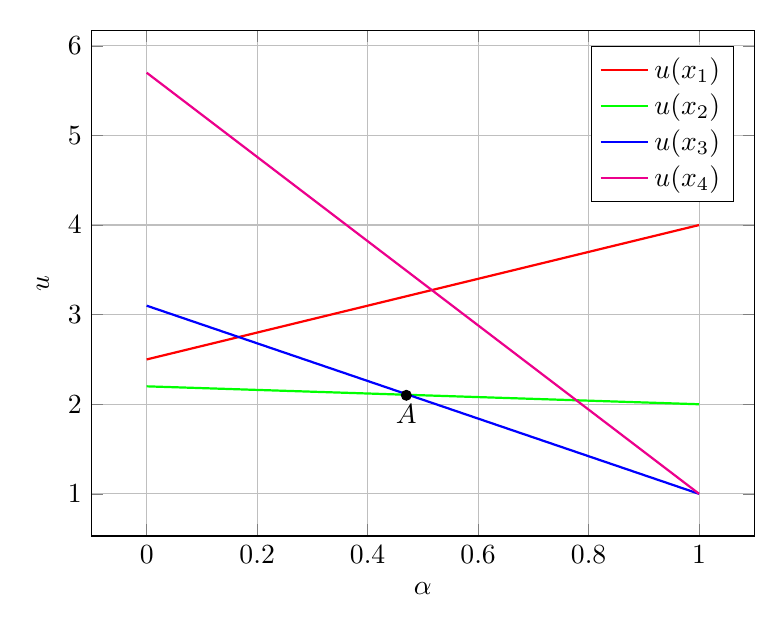
\begin{tikzpicture}
		\begin{axis}[
			xlabel={$\alpha$},
			ylabel={$u$},
			grid=major,
			legend pos=north east,
			domain=0:1,
			samples=100,
			width=10cm,
			height=8cm
			]
			%Functions
			\addplot[red, thick, name path=4] {2.5+1.5*x};
			\addlegendentry{$u(x_1)$}
			\addplot[green, thick, name path=1] {2.2-0.2*x};
			\addlegendentry{$u(x_2)$}
			\addplot[blue, thick, name path=2] {3.1-2.1*x};
			\addlegendentry{$u(x_3)$}
			\addplot[magenta, thick, name path=3] {5.7-4.7*x};
			\addlegendentry{$u(x_4)$}
			\fill (0.47,2.1) circle (2pt) node[below] {$A$};
		\end{axis}
	\end{tikzpicture}
\end{center}

Two solutions have nonempty support (the ones with no other functions below), and the threshold is obtained by intersecting their impact values
$$ 2.2 - 0.2 \alpha = 3.1 - 2.1 \alpha \implies \alpha = \frac{9}{19} $$
So that $\supp\left(x^{(2)}\right) = \left[0, \frac{9}{19}\right]$ and $\supp\left(x^{(3)}\right) = \left[\frac{9}{19}, 1\right]$.

\section{Formal defects of the expected value criterium}
\label{sec:formdefexpectedvalue}

Since the Seventeenth century, the expected value criterium was criticized for the unrealistic consequences (sometimes even paradoxical) it leads to.

Some strong defects of the expected value criterium:
\begin{enumerate}
	\item The actual preferences are inconsistent with the expected values
	
	\item Extreme values of probability and impact have paradoxical effects
\end{enumerate}

\subsection{Inconsistency between expected value and actual preferences}

According to the expected value criterium, all the combinations of impacts and probabilities producing the same result are reciprocally indifferent. In practice, this is often false: if one proposes to a decision-maker different combinations of impacts and probabilities with the same expected value, nearly always the decision maker shows a preference, even if this changes depending on the decision-maker. 

Consider the following alternatives:
\begin{itemize}
	\item Throw a die and gain 100 Euros for all outcomes
	
	\item Throw a die and gain 200 Euros for 4,5 and 6
	
	\item Throw a die and gain 600 Euros for 6
	
	\item Throw a die and gain 200 Euros for 2,3,4,5,6 and -400 Euros for 1
\end{itemize}

All alternatives have equal expected value: $\phi_{EV} (x) = 100$, $\forall x \in X$, most decision-makers however would consider them very different.

\subsection{Infinite expected values and infinitesimal probabilities}

There are thought experiments which show inconsistencies between practical preferences and the expected value criterium when applied to situations in which some impacts are unlimitedly large and some probabilities are unlimitedly small. 

In general, with this method, combining small probabilities with large impacts looks problematic.

\paragraph{Saint Petersburg's Paradox} The situation concerns a gamble:
\begin{itemize}
	\item The gambler pays $P$ to take part to the game
	
	\item We flip a coin until a tail is obtained
	
	\item The gambler wins a sum depending on the number of flips before the end of the game
\end{itemize}

The model of the game is the following;
\begin{itemize}
	\item Alternatives: play or do not play
	
	\item Scenarios: the coin is flipped $k$ times obtaining heads before the first tail ($\Omega = \N$)
	
	\item Probability function: $\pi_k = \frac{1}{2^{k+1}}$
	
	\item Impact function: 
	\begin{itemize}
		\item if we do not play, $f(P, k) = 0$
		
		\item if we do play, $f(P,k) = 2^k - P$
	\end{itemize}
\end{itemize}
\textit{What is the largest $P$  one should be willing to pay to play the game?}

Let's apply the expected value criterium:
\begin{itemize}
	\item If we do not play, $\phi_{EV} (P) = 0$
	
	\item If we do play, $\phi_{EV} (P) = \sum_{k \in \N} \frac{2^k - P}{2^{k+1}} = \sum_{k \in \N} \frac{1}{2} - \sum_{k \in \N} \frac{P}{2^{k+1}} = + \infty$
\end{itemize}

Playing pays out an infinite gain: any cost $P$ is justified. However, in real life nobody would pay a large sum.

\paragraph{A possible way out} Bernouilli suggested not to multiply probabilities and impacts: 
\begin{itemize}
	\item For finite creatures the utility for a gain is not proportional to it
	
	\item The marginal increase in utility is decreasing
\end{itemize}

Bernouilli suggested that \textit{utility increases logarithmically with the gain}
$$ u = \log (f) $$

This solves the original Saint Petersburg's paradox, but not a variant with gains $f$ increasing more than exponentially at each coin flip.

The paradox disappears only when the utility function is upper bounded.

%End L17, p288 notes

\section{Stochastic utility theory}
\label{sec:stochastic}

We aim to overcome the limits of the expected value criterium, by introducing a number of desired properties (axioms) and building a choice criterium that by construction satisfies them. 

We assume:
\begin{itemize}
	\item A preference relation $\Pi$ that is a weak order with a known constant value function $u(f)$ (replaced by a cost $f$)
	
	\item An uncertain environment: $|\Omega| > 1$ with probabilistic information
	
	\item A single decision-maker: $|D| = 1 \implies \Pi_d$ reduces to $\Pi$
\end{itemize}

The basic idea is to assume that the decision-maker is able to establish a preference relation $\Pi$ not only between pairs of deterministic impacts, but also between pairs of uncertain impacts, described as random variables. \\

\begin{definition}
	We denote as \textbf{finite simple lottery} $\ell_{f, \pi}$ a pair of functions $(f(\omega), \pi (\omega))$, where $f(\omega): \Omega \rightarrow F$ is a random variable on a finite sample space $\Omega$, while $\pi (\omega): \Omega \rightarrow [0;1]$ is a probability function on $\Omega$.
\end{definition}

The set of all finite lotteries on $F$ and $\Omega$ is therefore  
$$ \lottset = F^{|\Omega|} \times \P (\Omega) $$
as it contains all pairs of vectors such that the former has $|\Omega|$ components  in $F$ and the latter belongs to the probability space on $\Omega$. 

In a decision problem in conditions of risk, each alternative $x \in X$ corresponds to a lottery $\ell (x) \in L_x \subset L_{f, \Omega}$
$$ x \leftarrow \ell (x) = \left(f(x, \omega_1), \pi (\omega_1)\right) \oplus \dots \oplus \left(f(x, \omega_r), \pi (\omega_r)\right)$$
where we skip the terms of zero probability for the sake of brevity. \textit{This notation is nonstandard}. \\

\begin{definition}
	We denote as \textbf{degenerate lottery} a lottery where a single scenario has probability of 1
	$$ \ell_f = (f, 1) $$
\end{definition}

A single deterministic impact in $F$ is equivalent to a degenerate lottery. \\

\begin{definition}
	We denote as \textbf{binary lottery} a lottery where two scenarios have positive probability
	$$ \ell_{f, \alpha, f'} = (f, \alpha) \oplus (f', 1-\alpha)$$
\end{definition}

The simple lottery set $\lottset$ extends by recursion to lottery with multiple phases, where the impact obtained in each scenario is allowed to be a lottery; only the final phase provides deterministic gains and losses. \\

\begin{definition}
	We denote as \textbf{compound lottery} a lottery whose impacts are other lotteries (possibly degenerate).
\end{definition}

Compound lotteries model
\begin{itemize}
	\item lotteries taken in subsequent phases
	
	\item decisions taken before a sequence of uncertain events
\end{itemize}

They admit a graphical tree representation with:
\begin{itemize}
	\item Uncertain events on the internal nodes
	
	\item Deterministic impacts on the leaves
	
	\item Conditional probabilities on the arcs
	
	\item Probabilities summing to 1 on the arcs going out of each node \\
\end{itemize}

\begin{definition}
	We denote as $\lottset$, the set of all possible lotteries, simple or compound, on $F$ and $\Omega$.
\end{definition}

Given a finite decision problem in condition of risk, for any generic alternative $\bar x \in X$, the impact $f(\bar x, \omega)$ and the probability $\pi$ respect the definition of finite lottery. Therefore, any $x \in X$ corresponds to a lottery $\ell (x) \in \lottset$ and a method allowing to compare lotteries also allows to compare alternatives.

\subsection{Fundamental axioms of stochastic utility}

The stochastic utility theory first defines the properties that a preference relation between lotteries should respect in order to be rational. Then it proves that only a well-determined family of preference relation satisfies such properties, and that such relations can be represented by real-valued consistent functions. In this way, the selection of an alternative (lottery) among the feasible ones is equivalent to the optimization of the consistent function. \\

\begin{definition}
	A \textbf{preference relation between lotteries} is a binary relation on the lottery set
	$$ \Pi  \subset 2^{\lottset \times \lottset} $$
\end{definition}

\begin{definition}
	A preference relation between lotteries $\Pi \subset 2^{\lottset \times \lottset}$ admits a \textbf{consistent stochastic utility function} $u: \lottset \rightarrow \R$ when, for every pair of lotteries $\ell$ and $\ell'$, the utility of the preferred one exceeds the utility of the other one
	$$ \ell \wpref{} \ell' \Leftrightarrow u(\ell) \geq u(\ell') $$
\end{definition}

Von Neumann and Morgenstern
\begin{enumerate}
	\item Assume the existence of a preference relation $\Pi$ on lotteries
	
	\item Impose suitable conditions on $\Pi$
	
	\item Build a stochastic utility function $u(\ell)$ that is consistent with $\Pi$
	
	\item Reduce the decision problem in conditions of risk to
	$$ \max u(\ell (x)) $$
	$$ x \in X \Leftrightarrow \ell (x) \in L_X $$
	where feasible region $X$ corresponds to the feasible lotteries $L_X \subset \lottset$
\end{enumerate}

The properties required from a rational preference between lotteries, or axioms of stochastic utility, are the following: 
\begin{enumerate}
	\item \textbf{Weak ordering:} the preference relation between lotteries $\Pi$ is reflexive, transitive and complete
	
	\item \textbf{Monotony:} lotteries (both simple and compound) that assign larger probabilities to better impacts or lotteries are preferable
	$$ \alpha \geq \beta \Leftrightarrow (\ell, \alpha) \oplus (\ell', 1 - \alpha) \wpref{} (\ell, \beta) \oplus (\ell', 1 - \beta), \quad \forall \ell \wpref{} \ell' $$
	
	\item \textbf{Continuity:} any intermediate impact between two lotteries admits an equivalent compound lottery with the two given ones as outcomes: 
	$$ \ell \wpref{} f \wpref{} \ell' \implies \exists \alpha \in [0;1] : f \sim (\ell, \alpha) \oplus (\ell', 1 - \alpha) $$
	For any intermediate impact between lotteries, there exists a suitable probability value which allows to compose the two given lotteries into a lottery indifferent to the impact. Changing in a continuous way the probabilities modifies the preference continuously, leaving no impact "uncovered".
	
	\item \textbf{Independence} (or \textbf{substitution})\textbf{:} the preference between two lotteries does not change combining them with the same lottery with the same probability:
	$$ \ell \wpref{} \ell' \Leftrightarrow (\ell, \alpha) \oplus (\ell'', 1 - \alpha) \wpref{} (\ell', \alpha) \oplus (\ell'', 1-\alpha), \quad \forall \alpha \in (0;1] $$
	
	\item \textbf{Reduction:} any compound lottery is indifferent to the simple lottery with: 
	\begin{itemize}
		\item the same final impacts
		
		\item probabilities given by the laws of
		\begin{itemize}
			\item conditional probabilities: multiply along each path
			
			\item total probabilities: sum on disjoint path
		\end{itemize}
	\end{itemize}
	Impacts and probabilities are relevant, the lottery structure is not. Basically, we can keep just a simple lottery with all final impacts and probabilities suitably adjusted.
\end{enumerate}

\subsection{Von Neumann-Morgenster stochastic utility theorem}

The following theorem proves that, under the axioms discussed above, it's always possible to build a consistent stochastic utility function to compare lotteries. Moreover, it's possible to build infinitely many such functions, that coincide with one another up to a linear scaling, so that there is one and only one normalized utility function. Since the proof is constructive, it also shows how to build such function. \\

\begin{theo}
	Given a set of impacts $F$ not all reciprocally indifferent, a sample space $\Omega$ and a preference relation $\Pi$ between lotteries on $F$ and $\Omega$ that respects the five axioms of Von Neumann and Morgenstern, there exists one and only one utility function $u (\ell): \lottset \rightarrow [0,1]$ consistent with $\Pi$ and normalized so as to have value 0 in the worst impact and 1 in the best impact.
\end{theo}

\begin{proof}
	The existence of a weak order on $F$ guarantees that there exists at least one worst impact $f^\dag$ and one best impact $f^\circ$ in $F$. Let $\ell^\dag = (f^\dag, 1)$ be the degenerate lottery that certainly returns the worst impact and $\ell^\circ = (f^\circ, 1)$ the degenerate lottery that certainly returns the best impact.  Since all impacts are not reciprocally indifferent
	$$ f^\circ \prec f^\dag \ \text{ that is } \ \ell^\circ \prec \ell^\dag $$
	
	Now we can assign extreme conventional values to the utility of these two lotteries
	$$ u(\ell^\dag) = 0 \ \text{ and } \ u(\ell^\circ) = 1 $$
	
	As a second step, we build the utility values for all degenerate lotteries, that is for all impacts in $F$, exploiting the continuity axiom. For every impact $f \in F$ there exists certainly a probability $\alpha_f \in [0;1]$ that produces a lottery between the two extreme impacts and is indifferent with respect to the degenerate lottery corresponding to $f$: 
	$$ \exists \alpha_f \in [0;1] : (\ell^\circ, \alpha_f) \oplus (\ell^\dag, 1 - \alpha_f) \sim f $$
	
	The value of $\alpha_f$ is unique thanks to the monotony axiom.
	
	As a third step, we build utility values for general lotteries. In order to do that, we exploit the substitution and reduction axioms. Every possible final impact $f \in F$ of a lottery can be seen as a degenerate lottery $\ell_f$, which is equivalent to a binary lottery $(\ell^\circ, \alpha_f) \oplus (\ell^\dag, 1 - \alpha_f)$ between the extreme impacts. Given a general lottery $\ell$ each of its final impacts $f$ can be replaced with the degenerate lottery or with the equivalent binary lottery obtaining a compound two-phase lottery. The first phase no longer provides the single impacts, but tickets to take part to the second phase, in which only extreme impacts $f^\circ$ and $f^\dag$ are possible.
	
	The reduction axiom allows to combine the two phases into a single lottery with the same final impacts (the two extreme ones) and probabilities determined by the theorem of total probability. Now, the given lottery $\ell$ corresponds to a simple lottery between the extreme impacts
	$$ \ell \sim \left(f^\circ, \sum_{\omega \in \Omega} \pi_\omega \alpha_{f(\omega)} \right) \oplus \left(f^\dag, 1 - \sum_{\omega \in \Omega} \pi_\omega \alpha_{f(\omega)}\right) $$
	
	We define the utility lottery $\ell$ as the probability of the best impact $\ell^\circ$. Since $\alpha_f = u(\ell_f)$, the stochastic utility of a lottery coincides with the expected value of the utility of the impact
	$$ u(\ell) = \sum_{\omega \in \Omega} \pi_\omega u(f(\omega)) = E \left[u(f)\right] $$
\end{proof}

The utility of a lottery is the expected value of the utility in the scenarios, \textit{as Bernouilli proposed, combine perceived utilities, not impacts}.

In summary, the Von Neumann-Morgenstern theorem
\begin{itemize}
	\item Receives from the decision-maker $u(f)$ for all $f \in F$
	
	\item Returns $u(\ell)$ for all $\ell \in L$
\end{itemize}

Since in a decision problem an alternative is a lottery, we pick the maximum expected value (benefits).

Stochastic utility and multi-attribute utility exhibit strong similarities:
\begin{itemize}
	\item They are convex combinations of utilities with coefficients
	
	\item The utilities are normalized between a worst and best impact
	
	\item The coefficients are normalized between 0 and 1 with unitary sum
\end{itemize}

But there are also strong differences:
\begin{itemize}
	\item Additivity is intrinsically satisfied (no special condition required) because the different scenarios do not interact, while indicators do
	
	\item The attribute set $P$ is replaced by scenario set $\Omega$, possibly infinite
	
	\item The weights $w_l$ are replaced by probabilities $\pi (\omega)$ that do not necessarily require the decision-maker (they might be frequencies)
\end{itemize}

\section{Risk aversion and risk propensity}
\label{sec:riskaversion}

\begin{definition}
	We denote as \textbf{risk profile} the profile of the stochastic utility function on the degenerate lotteries $\ell_f$ as impact $f$ varies in $F$.
\end{definition}

The shape of $u(f)$ for all $f \in F$, it determines $u(\ell(f, \pi))$ for all $\ell \in L$, combining $u(f)$ and $\pi (\omega)$, therefore \textit{showing the attitude of the decision-maker} towards risk.

For the sake of simplicity, we'll assume that
\begin{itemize}
	\item $f$ is a benefit
	
	\item The impact set is an interval $F = \left[f^\dag, f^\circ\right]$
	
	\item Consequently, the risk profile increases from $(f^\dag, 0)$ to $(f^\circ, 0)$
\end{itemize}

The extension to more general cases is possible.

Now consider: 
\begin{itemize}
	\item An intermediate deterministic impact $f_\alpha = (1 - \alpha) f^\dag + \alpha f^\circ$
	
	\item A binary lottery $\ell_{f^\circ, \alpha, f^\dag}$ combining $f^\circ$ and $f^\dag$ with coefficient $\alpha$
\end{itemize}

They are equivalent for the expected value criterium
$$ \phi_{EV} (f_\alpha) = f_\alpha = \phi_{EV} \left(\ell_{f^\circ, \alpha, f^\dag}\right)$$

\textit{What about their stochastic utilities $u(f_\alpha)$ and $u \left(\ell_{f^\circ, \alpha, f^\dag}\right)$?} The utility of any binary lottery $\ell_{f^{(1)}, \alpha, f^{(2)}}$ can be computed from the segment between points $\left(f^{(1)}, u\left(f^{(1)}\right)\right)$ and  $\left(f^{(2)}, u\left(f^{(2)}\right)\right)$
$$ u \left(\ell_{f^\circ, \alpha, f^\dag}\right) = \alpha u \left(f^\circ\right) + \left(1 - \alpha\right)u \left(f^\dag\right) $$

Three relevant cases (not exhaustive) exist: 
\begin{enumerate}
	\item \textbf{Convex case:} the risk profile is above the segment from $(f^\dag, 0)$ to $(f^\circ, 1)$ and the lottery is preferred to the deterministic impact
	$$ u\left(f_\alpha\right) \leq u \left(\ell_{f^\circ, \alpha, f^\dag}\right), \quad \forall \alpha \in [0,1] $$
	The decision maker is \textit{risk-prone}
	
	\item \textbf{Linear case:} the risk profile is lying on the segment from $(f^\dag, 0)$ to $(f^\circ, 1)$ and the lottery and the deterministic impact are equivalent
	$$ u\left(f_\alpha\right) = u \left(\ell_{f^\circ, \alpha, f^\dag}\right), \quad \forall \alpha \in [0,1] $$
	The decision-maker is \textit{risk-neutral, the expected value criterium is confirmed}
	
	\item \textbf{Concave case:} the risk profile is below the segment from $(f^\dag, 0)$ to $(f^\circ, 1)$ and the deterministic impact is preferred to the lottery 
	$$ u\left(f_\alpha\right) \geq u \left(\ell_{f^\circ, \alpha, f^\dag}\right), \quad \forall \alpha \in [0,1] $$
	The decision-maker is \textit{risk-averse}
\end{enumerate}

\subsection{Certainty equivalent and risk premium}

An equivalent description of the risk profile of a decision-maker is given by the inverse of the utility function, that is the function that rebuilds an impact $f(u)$ for each possible value of the stochastic utility $u$. This inverse function certainly exists, given that $u(f)$ is strictly increasing. \\

\begin{definition}
	Given a lottery $\ell$ we denote as \textbf{certainty equivalent} the deterministic impact $f_\ell$ that is equivalent to the lottery, and \textbf{risk premium} the difference between the expected value of the lottery and its certainty equivalent.
\end{definition}

The certainty equivalent can differ from the expected value of the impact. Given a lottery $\ell$ of utility $u$: 
\begin{itemize}
	\item The expected value of the impact is $\phi_{EV} (\ell) = E \left[f(\ell, \omega)\right]$
	
	\item The certainty equivalent is $CE(\ell) = f(u(\ell))$
\end{itemize}

The risk premium $RP(\ell)$ is the difference of the two terms
$$ RP(\ell) = \phi_{EV} (\ell) - CE(\ell) = E\left[f(\ell, \omega)\right] - f(u(\ell)) $$

The risk premium measures the additional utility that the decision-maker requires in order to accept a lottery instead of its expected value. Therefore: 
\begin{itemize}
	\item For risk-averse decision-makers, the certainty equivalent of a lottery is smaller than its expected value, and the risk premium is positive
	
	\item For risk-neutral decision-makers, the certainty equivalent of a lottery is equal to its expected value, and the risk premium is zero 
	
	\item For risk-prone decision-makers, the certainty equivalent of a lottery is larger than its expected value, and the risk premium is negative
\end{itemize}

%End L18, p299 notes
	
\end{document}